%%% The main file. It contains definitions of basic parameters and includes all other parts.

%% Settings for single-side (simplex) printing
% Margins: left 40mm, right 25mm, top and bottom 25mm
% (but beware, LaTeX adds 1in implicitly)
\documentclass[12pt,a4paper]{report}
\setlength\textwidth{145mm}
\setlength\textheight{247mm}
\setlength\oddsidemargin{15mm}
\setlength\evensidemargin{15mm}
\setlength\topmargin{0mm}
\setlength\headsep{0mm}
\setlength\headheight{0mm}
% \openright makes the following text appear on a right-hand page
\let\openright=\clearpage

\setlength{\emergencystretch}{10cm}
\pretolerance=10000
\tolerance=10000
\hfuzz=5000pt
\vfuzz=5000pt 

%% Settings for two-sided (duplex) printing
% \documentclass[12pt,a4paper,twoside,openright]{report}
% \setlength\textwidth{145mm}
% \setlength\textheight{247mm}
% \setlength\oddsidemargin{14.2mm}
% \setlength\evensidemargin{0mm}
% \setlength\topmargin{0mm}
% \setlength\headsep{0mm}
% \setlength\headheight{0mm}
% \let\openright=\cleardoublepage

%% Generate PDF/A-2u
\usepackage[a-2u]{pdfx}

%% Character encoding: usually latin2, cp1250 or utf8:
\usepackage[utf8]{inputenc}

%% Prefer Latin Modern fonts
\usepackage{lmodern}

%% Further useful packages (included in most LaTeX distributions)
\usepackage{amsmath}        % extensions for typesetting of math
\usepackage{amsfonts}       % math fonts
\usepackage{amsthm}         % theorems, definitions, etc.
\usepackage{bbding}         % various symbols (squares, asterisks, scissors, ...)
\usepackage{bm}             % boldface symbols (\bm)
\usepackage{graphicx}       % embedding of pictures
\usepackage{fancyvrb}       % improved verbatim environment
\usepackage{natbib}         % citation style AUTHOR (YEAR), or AUTHOR [NUMBER]
\usepackage[nottoc]{tocbibind} % makes sure that bibliography and the lists
			    % of figures/tables are included in the table
			    % of contents
\usepackage{dcolumn}        % improved alignment of table columns
\usepackage{booktabs}       % improved horizontal lines in tables
\usepackage[usenames, dvipsnames]{xcolor}  % typesetting in color



% Packages added by Dahn
\usepackage[colorinlistoftodos,prependcaption,textsize=tiny,disable]{todonotes} % disable
\usepackage{xargs}
\usepackage{bbm}	% For lowercase blackboard bold
\usepackage{multicol}  	% ultiple columns
\usepackage{enumerate}
\usepackage{amssymb}	% \varnothing
\usepackage{booktabs}
\newcommand{\ra}[1]{\renewcommand{\arraystretch}{#1}} % For line stretching in booktabs
\usepackage{lscape}
\usepackage[overlay,absolute]{textpos}
\usepackage{pgf,tikz,pgfplots}
\pgfplotsset{compat=1.15}
\usetikzlibrary{arrows}
\usepackage{breakcites}

\newcommand\PlaceText[3]{%
\begin{textblock*}{10in}(#1,#2)  %% change width of box from 10in as you wish
#3
\end{textblock*}
}%
\textblockorigin{-5mm}{0mm} 

% Dahn commands
\newcommand{\Rd}{{\mathbb R^d}}
\newcommand{\Rt}{{\mathbb R^3}}

\newcommandx{\problem}[2][1=]{\todo[linecolor=red,backgroundcolor=red!25,bordercolor=red,#1]{#2}}
\newcommandx{\todoo}[2][1=]{\todo[linecolor=blue,backgroundcolor=blue!25,bordercolor=blue,#1]{#2}}
\newcommandx{\note}[2][1=]{\todo[linecolor=OliveGreen,backgroundcolor=OliveGreen!25,bordercolor=OliveGreen,#1]{#2}}
\newcommandx{\unsure}[2][1=]{\todo[linecolor=Plum,backgroundcolor=Plum!25,bordercolor=Plum,#1]{#2}}

\newtheorem{theorem}{Theorem}

\theoremstyle{definition}
\newtheorem{definition}{Definition}

\theoremstyle{remark}
\newtheorem{remark}{Remark}

\theoremstyle{theorem}
\newtheorem{proposition}{Proposition}

\theoremstyle{remark}
\newtheorem{ex}{Example}


\newcommand{\tbd}{\textbf{{\color{red}~ TO BE DONE ~}}}

\newcommand{\x}{{\mathbf{x}}}
\newcommand{\p}{{\mathbbm{p}}}

%% Augumented matrix 
\newenvironment{amatrix}[1]{%
  \left(\begin{array}{@{}*{#1}{c}|c@{}}
}{%
  \end{array}\right)
}


\newenvironment{tight_enumerate}{
\begin{enumerate}
  \setlength{\itemsep}{0pt}
  \setlength{\parskip}{0pt}
}{\end{enumerate}}

%%% Basic information on the thesis

% Thesis title in English (exactly as in the formal assignment)

\def\ThesisTitle{Generalized random tessellations, their properties, simulation and applications}

% Author of the thesis
\def\ThesisAuthor{Daniel Jahn}

% Year when the thesis is submitted
\def\YearSubmitted{2019}

% Name of the department or institute, where the work was officially assigned
% (according to the Organizational Structure of MFF UK in English,
% or a full name of a department outside MFF)
\def\Department{Department of Probability and Mathematical Statistics}

% Is it a department (katedra), or an institute (ústav)?
\def\DeptType{Department}

% Thesis supervisor: name, surname and titles
\def\Supervisor{prof. RNDr. Viktor Bene\v{s}, DrSc.}

% Supervisor's department (again according to Organizational structure of MFF)
\def\SupervisorsDepartment{Department of Probability and Mathematical Statistics}

% Study programme and specialization
\def\StudyProgramme{Mathematics}

% An optional dedication: you can thank whomever you wish (your supervisor,
% consultant, a person who lent the software, etc.)
\def\Dedication{%
I would like to thank my supervisor prof. RNDr. Viktor Bene\v{s}, DrSc. for all the time and effort he put into helping me on the often thorny path of writing this thesis. I am also grateful for all the opportunities he provided me with to present and discuss my work on seminars and conferences.

If there is one other person without whom this thesis would have been much more difficult to write, it is my partner, Adela Nguy$\tilde{\hat{e}}$n. I am grateful for having her by my side throughout the whole process of writing this thesis. She has far surpassed the official requirements for the partner of a mathematician, that is to be emotionally supportive and understanding, especially when waking up in the middle of the night to find the said mathematician working, again. She has spent countless hours listening to me talk about circles and tetrahedrons and, on several occasions, picked up a pen and paper and actively helped me solve the problems. Thank you for everything.

For helping me with a difficult programming language I knew nothing about, as well as for general advice on programming, I thank my friend and an excellent programmer Jan Noha.

I thank Colin Beet for helping me improve the linguistic aspects of this thesis. He would like the reader to know that, contrary to what Remark \ref{r:abuse} claims, abuse of any kind can never be justified.

I thank my family for supporting my academic endeavours even though they still have no idea what it is I am actually doing. 

Finally, I'd like to thank the following people who have provided valuable insights and comments: Prof. David Dereudre, Jeremy Tan, Mat\v{e}j Kov\'{a}\v{r}, Prof. Volker Schmidt, Prof. David Eppstein.
}


% Abstract (recommended length around 80-200 words; this is not a copy of your thesis assignment!)
\def\Abstract{%
	The past few years have seen advances in modelling of polycrystalline materials using parametric tessellation models from stochastic geometry. A promising class of tessellations, the Gibbs-type tessellation, allows the user to specify a great variety of properties through the energy function. 
	This text focuses solely on Gibbs-type tetrahedrizations, a three-dimensional tessellation composed of tetrahedra. The existing results for two-dimensional Delaunay triangulations are extended to the case of three-dimensional Laguerre tetrahedrization. We provide a proof of existence, a \texttt{C++} implementation of the MCMC simulation and estimation of the models parameters through maximum pseudolikelihood.
}

% 3 to 5 keywords (recommended), each enclosed in curly braces
\def\Keywords{%
	{Gibbs point process} {tetrahedrization} {Laguerre}  {existence} {simulation} {maximum pseudolikelihood estimation}
}

%% The hyperref package for clickable links in PDF and also for storing
%% metadata to PDF (including the table of contents).
%% Most settings are pre-set by the pdfx package.
\hypersetup{unicode}
\hypersetup{breaklinks=true}

% Definitions of macros (see description inside)
%%% This file contains definitions of various useful macros and environments %%%
%%% Please add more macros here instead of cluttering other files with them. %%%

%%% Minor tweaks of style

% These macros employ a little dirty trick to convince LaTeX to typeset
% chapter headings sanely, without lots of empty space above them.
% Feel free to ignore.
\makeatletter
\def\@makechapterhead#1{
  {\parindent \z@ \raggedright \normalfont
   \Huge\bfseries \thechapter. #1
   \par\nobreak
   \vskip 20\p@
}}
\def\@makeschapterhead#1{
  {\parindent \z@ \raggedright \normalfont
   \Huge\bfseries #1
   \par\nobreak
   \vskip 20\p@
}}
\makeatother

% This macro defines a chapter, which is not numbered, but is included
% in the table of contents.
\def\chapwithtoc#1{
\chapter*{#1}
\addcontentsline{toc}{chapter}{#1}
}

% Draw black "slugs" whenever a line overflows, so that we can spot it easily.
\overfullrule=1mm

%%% Macros for definitions, theorems, claims, examples, ... (requires amsthm package)

\theoremstyle{plain}
\newtheorem{thm}{Theorem}
\newtheorem{lemma}[thm]{Lemma}
\newtheorem{claim}[thm]{Claim}

\theoremstyle{plain}
\newtheorem{defn}{Definition}

\theoremstyle{remark}
\newtheorem*{cor}{Corollary}
\newtheorem*{rem}{Remark}
\newtheorem*{example}{Example}

%%% An environment for proofs

%%% FIXME %%% \newenvironment{proof}{
%%% FIXME %%%   \par\medskip\noindent
%%% FIXME %%%   \textit{Proof}.
%%% FIXME %%% }{
%%% FIXME %%% \newline
%%% FIXME %%% \rightline{$\square$}  % or \SquareCastShadowBottomRight from bbding package
%%% FIXME %%% }

%%% An environment for typesetting of program code and input/output
%%% of programs. (Requires the fancyvrb package -- fancy verbatim.)

\DefineVerbatimEnvironment{code}{Verbatim}{fontsize=\small, frame=single}

%%% The field of all real and natural numbers
\newcommand{\R}{\mathbb{R}}
\newcommand{\N}{\mathbb{N}}

%%% Useful operators for statistics and probability
\DeclareMathOperator{\pr}{\textsf{P}}
\DeclareMathOperator{\E}{\textsf{E}\,}
\DeclareMathOperator{\var}{\textrm{var}}
\DeclareMathOperator{\sd}{\textrm{sd}}

%%% Transposition of a vector/matrix
\newcommand{\T}[1]{#1^\top}

%%% Various math goodies
\newcommand{\goto}{\rightarrow}
\newcommand{\gotop}{\stackrel{P}{\longrightarrow}}
\newcommand{\maon}[1]{o(n^{#1})}
\newcommand{\abs}[1]{\left|{#1}\right|}
\newcommand{\dint}{\int_0^\tau\!\!\int_0^\tau}
\newcommand{\isqr}[1]{\frac{1}{\sqrt{#1}}}

%%% Various table goodies
\newcommand{\pulrad}[1]{\raisebox{1.5ex}[0pt]{#1}}
\newcommand{\mc}[1]{\multicolumn{1}{c}{#1}}


% Title page and various mandatory informational pages
\begin{document}
%%% Title page of the thesis and other mandatory pages

%%% Title page of the thesis

\pagestyle{empty}
\hypersetup{pageanchor=false}
\begin{center}

\centerline{\mbox{
\includegraphics[width=166mm]{../img/logo-en.pdf}}}

\vspace{-8mm}
\vfill

{\bf\Large MASTER THESIS}

\vfill

{\LARGE\ThesisAuthor}

\vspace{15mm}

{\LARGE\bfseries\ThesisTitle}

\vfill

\Department

\vfill

\begin{tabular}{rl}

Supervisor of the master thesis: & \Supervisor \\
\noalign{\vspace{2mm}}
Study programme: & \StudyProgramme \\
\noalign{\vspace{2mm}}
Study branch: & Probability, mathematical statistics \\
& and econometrics \\
\end{tabular}

\vfill

% Zde doplňte rok
Prague \YearSubmitted

\end{center}

\newpage

%%% Here should be a bound sheet included -- a signed copy of the "bachelor
%%% thesis assignment". This assignment is NOT a part of the electronic
%%% version of the thesis. DO NOT SCAN.

%%% A page with a solemn declaration to the bachelor thesis

\openright
\hypersetup{pageanchor=true}
\pagestyle{plain}
\pagenumbering{roman}
\vglue 0pt plus 1fill

\noindent
I declare that I carried out this master thesis independently, and only with the cited
sources, literature and other professional sources.

\medskip\noindent
I understand that my work relates to the rights and obligations under the Act No.~121/2000 Sb.,
the Copyright Act, as amended, in particular the fact that the Charles
University has the right to conclude a license agreement on the use of this
work as a school work pursuant to Section 60 subsection 1 of the Copyright Act.

\vspace{10mm}

\hbox{\hbox to 0.5\hsize{%
In ........ date ............	% FIXME!
\hss}\hbox to 0.5\hsize{%
signature of the author
\hss}}

\vspace{20mm}
\newpage

%%% Dedication

\openright

\noindent
\Dedication

\newpage

%%% Mandatory information page of the thesis

\openright

\vbox to 0.5\vsize{
\setlength\parindent{0mm}
\setlength\parskip{5mm}

Title:
\ThesisTitle

Author:
\ThesisAuthor

\DeptType:
\Department

Supervisor:
\Supervisor, \SupervisorsDepartment

Abstract:
\Abstract

Keywords:
\Keywords

\vss}

\newpage

\openright
\pagestyle{plain}
\pagenumbering{arabic}
\setcounter{page}{1}



%%% A page with automatically generated table of contents of the master thesis
\tableofcontents



%%%% Glossary
\chapwithtoc{Glossary of terms and abbreviations}
\subsubsection{Mathematical operators and notation}
The following list only serves as a reference. Most of the following terms are defined more precisely when they are first used in the text.

\hspace*{-8mm}
\begin{tabular}{ l l }
	$\mathbb N_0$ & $\mathbb N \cup \{0\}$ \\
	$B(x,r)$ & Open ball with center $x$ and radius $r$ \\
	$\mathrm{diam}(A)$ & Diameter of the set $A$; $sup_{x,y\in A}\|x-y\|$ \\
	$\mathrm{card}(A)$ & Cardinality of the set $A$ \\
	$\mathrm{conv}(A)$ & Convex hull of the set $A$ \\
	$\lambda(A), |A|$ & Lebesgue measure of the set A \\
	$\partial$ & Topological boundary of a set \\
	$A+B$ & Minkowski sum of the sets $A$ and $B$; the set $\{a+b: a\in A, b\in B\}$. \\
	$\mathrm{pr}_{\Rt}(\cdot)$ & Projection from $\mathbb R^4$ to $\Rt$ \\
	$\angle pqr$ & Angle formed by $pqr$ \\
	$\propto$ & Proportional to \\
	$\delta_x(A)$ & Dirac delta function at $x$. Equals to 1 if $x\in A$, 0 otherwise.\\ 
	$\mathrm{det} M$ & Determinant of the matrix $M$ \\
	$\| \cdot \|$ & Euclidean norm \\
	$d(p,x)$ & Power distance of the point $x$ and weighted point $p$ \\
	$\rho(p,q)$ & Power product of two weighted points $p$ and $q$ \\
	$\chi(\eta)$ & For $\mathrm{card}(\eta)=4$, circumdiameter of the tetrahedron $\mathrm{conv}(\eta)$.\\
\end{tabular}




\subsubsection{Abbreviations}
\begin{tabular}{ l l }
	DLR & Dobrushin-Lanford-Ruelle (equations) \\
	GNZ & Georgii-Nguyen-Zessin (equation) \\
	MCMC & Markov chain Monte carlo \\
	MPLE & Maximum pseudolikelihood estimation
\end{tabular}




%%% Each chapter is kept in a separate file
\chapter*{Introduction}
\addcontentsline{toc}{chapter}{Introduction}

An important area in materials science is the study of polycrystalline materials. Advances in understanding now allow us to accurately characterize the macro-scale properties of such materials using only their microscopic structure. It is therefore essential to develop adequate mathematical models to accurately capture and describe the microscopic properties of these materials.
Stochastic models have provided an extremely useful way of capturing the irregularities of the real world, and the study of polycrystalline materials is no different. In particular, the random tessellation models from stochastic geometry have proven to be especially appropriate for the mosaic-like grain structure of polycrystalline materials. 

This work, as a part of the project solution of GACR 17-00393J (investigator V. Bene\v{s}), studies a type of tessellations closely related to the grain structure of polycrystalline materials --- tetrahedrizations, in particular Gibbs-type tetrahedrizations. These tessellations based on the Gibbs point process allow a great flexibility in modelling the different properties of the resulting structure. 
The main contribution of this text is twofold. 

The practical contribution is an extension of the work done in \cite{DereudreLavancier2011}. The two-dimensional Gibbs-Delaunay model used there is extended here to three dimensions and further generalized to Gibbs-Laguerre-Delaunay, a tessellation model which allows to attach a weight to each point. In Chapters \ref{ch:simulation} and \ref{ch:estimation}, we present the approach used in simulation of parametric tessellation models and estimation of their parameters. Chapter \ref{ch:numeric} then presents the numerical results. However, these three chapters a merely a report of the most important part of the work not present in this text --- the \texttt{C++} implementation, see Appendix \ref{appendix:implementation} for more details. 

The theoretical contribution of this text are the proofs of existence of the Gibbs-Laguerre-Delaunay models used. Using the work in \cite{DDG12} the intricate interactions present in our models are analyzed through the hypergraph structures they generate. The proofs themselves can be found in Theorems \ref{thm:E1}-\ref{thm:E4} in Chapter \ref{ch:3}. However, all of Section \ref{sec:verifyassumptions} as well as Section \ref{sec:boundingdiameter} are composed of original work. 

Finally, Chapters \ref{ch:1} and \ref{ch:2} contain the necessary theoretical background. We would in particular like to draw attention to Section \label{sec:Laguerre} which provides a stand-alone presentation of the theory Laguerre tetrahedrization without relying on its duality to Laguerre tessellation, as the existing literature does, and thus provides a direct understanding of the structure. 

\todoo[inline]{Glossary of terms and abbreviations}

\chapter{Geometric preliminaries}\label{ch:1}
Before diving into the mathematics of Gibbs-Laguerre-Delaunay tetrihedrization models, we must first lay out the fundamentals of their geometric and combinatorial structure. The key geometric components are the the circumball for Delaunay tetrahedrizations and characteristic point for Laguerre tetrahedrizations. We will first study their geometry and then analyze their structure in terms of hypergraphs.

\subsubsection{Notation and basic terms}
This text will predominantly focus on \textit{marked} points in $\Rt$, that is elements of $\Rt \times S$, where $S=[0,W],W>0$ is the \textit{mark set}. A great deal of care must be dedicated to clearly distinguish between \textit{positions} of points (their projection to $\Rt$) and their \textit{marks}\footnote{Marks will also be often called weights.} (projection to $S$). To this end, we adopt the following notation. A point $p \in \Rt\times S$ has the position $p'\in \Rt$ and mark $p'' \in S$. Similarly, the notation of sets follows accordingly --- the Borel $\sigma$-algebra on $\Rt\times S$ will be denoted $\mathcal B$, its counterpart on $\Rt$ will be denoted $\mathcal B'$. The subset of $\mathcal B$ ($\mathcal B'$) containing only bounded sets is $\mathcal B_0$ ($\mathcal B_0'$). 

A \textit{configuration} is a set $\x \in \mathbf N_{lf}$, where 
$$\mathbf N_{lf} = \{\x \subset \Rt\times S: \mathrm{card}(\x \cap B) < \infty, B\in \mathcal B_0\} $$ 
be the set of locally finite sets on $\Rt\times S$. Let $\mathbf N_{f} \subset \mathbf N_{lf}$ be the set of all finite sets on $\Rt\times S$. Lastly, for $\Lambda \in \mathcal B_0'$, playing the role of the observation window, denote 
$$\mathbf N_\Lambda = \{ \x \in \mathbf N_{f}: \x'\subset \Lambda\}.$$
A subset of $\x$ will be denoted $\eta$. If $\mathrm{card}(\eta)=4$, then $\eta$ is \textit{tetrahedral} or a \textit{tetrahedron}. The symbols $\x'=\mathrm{pr_{\Rt}}(\x), \eta'=\mathrm{pr_{\Rt}}(\eta)$ again refer only to the positional part. 

\todoo[inline]{Probably comment here on the fact that $|\Lambda|$ will be assumed to be positive}

\section{Tetrahedrizations}\label{sec:tetrahedrizations}
The aim of this section is to introduce the geometric concepts necessary for the understanding of two types of tetrahedrizations: Delaunay and Laguerre. The main focus of this text lies on the Laguerre tetrahedrization and thus Delaunay tetrahedrization will receive significantly less attention and often will be treated only as a special case. Note that although this text focuses solely on the three dimensional case, most ideas remain valid for a triangulation in any dimension.\todoo{Reference some resources on Delaunay and Laguerre-Delaunay} 

We introduce the notion of (reinforced) general position, a traditional assumption on configurations.

\begin{definition}
Let $\x \in \mathbf N_{lf}$. We say $\x$ is in \textbf{general position} if 
$$ \eta \subset \x, 2 \leq \mathrm{card}(\eta) \leq 3 \Rightarrow \eta' \text{ is affinely independent in } \Rt. $$   
Denote $\mathbf N_{gp}\subset \mathbf N_{lf}$ the set of all locally finite configurations in general position.
\end{definition}
\todoo[inline]{Comment on the fact that we need a vector space with measurable inner product etc?}
\note[inline]{It's sufficient to check only subsets with $d+1$ points}
 
\begin{definition}
Let $\x \in \mathbf N_{gp}$. We say $\x$ is in \textbf{reinforced general position} if 
$$ \eta \subset \x, 3 \leq \mathrm{card}(\eta) \leq 4 \Rightarrow \eta' \text{ is not cocircular.} $$   
Denote $\mathbf N_{rgp}$ the set of all locally finite configurations in reinforced general position.
\end{definition}
\todoo[inline]{This definition is possibly not even needed}
\note[inline]{Again, only need to check $d+2$}


\subsection{Delaunay tetrihedrization}
This section will shortly introduce the three dimensional equivalent of the well known Delaunay triangulation.\todoo{Add references to resources} While the configurations in this section are technically marked sets, none of the terms take marks into consideration, as the Delaunay tetrahedrization relies on positions only.

\begin{definition}
	Let $\x \in \mathbf N_{gp}$, $\eta \subset \x$. An open ball $B(\eta,\x)$ such that $\eta' \subset \partial B(\eta,\x)$ is called a \textit{circumball of $\eta$}. The boundary $\partial B(\eta,\x)$ is called a \textit{circumsphere}.
	Let $\eta\subset\x$, $\mathrm{card}(\eta)=4$, be a tetrahedron. Then we will denote its (uniquely defined) circumball as $B(\eta)$ as its definition does not depend on $\x$. 
\end{definition}	

\begin{definition}
	Let $\x \in \mathbf N_{gp}$ and $\eta \subset \x$. We say that $(\eta,\x)$ satisfies the \textit{empty ball property} if $B(\eta,x) \cap \x' = \emptyset$. 
	For convenience, for $\x \in \mathbf N_{lf}\setminus \mathbf N_{gp}$, we define any $\eta\subset \x$ that does not satisfy the assumptions of general position as not satisfying the empty ball property.
\end{definition}

\begin{definition}
	Let $\x \in \mathbf N_{lf}$. Define the set 
	$$\mathcal {D}(\x) := \{\eta\subset \x: \eta \text{ satisfies the empty ball property }\}.$$
	and its subsets
	$$\mathcal {D}_k(\x) := \{\eta \in \mathcal {D}(\x): \mathrm{card}(\eta)=k \},\quad k = 1,\dots,4.$$
	We then define the \textit{Delaunay tetrihedrization of $\x$} as the set $\mathcal D_4(\x)$. 
\end{definition}

The set $\mathcal D_4$ contains the structure we would expect from the name tetrihedrization, namely it contains sets of 4-tuples of points whose convex hull are the tetrahedra forming the Delauany tetrihedrization. The fact that we've defined the set $\mathcal D_k(\x)$ for any $k=1,\dots,4$ reflects the hypergraph approach to these structures presented in section \ref{sec:hypergraphs}.

\todoo[inline]{Possibly remark on existence and uniqueness, although this is not that interesting under this definition}

The following proposition shows one important property of the set $\mathcal D_2(\x)$ for any $\x \in \mathbf N_{lf}$ --- it contains the edges of the (undirected) nearest neighbor graph.
\begin{proposition}\label{prop:nng}
	Define 
	$$\mathrm{NNG}(\x) = \big\{ \{p,q\}\subset \x \times \x: p\neq q, \|p-q\| \leq \|p-s\|, s\in \x\setminus\{p\}  \big\}.$$
	Then 
	$$\mathrm{NNG}(\x) \subset \mathcal D_2(\x).$$
\end{proposition}
\begin{proof}
	Let $\x\in \mathbf N_{lf}$ and $\eta =\{p,q\} \in \mathrm{NNG}(\x)$. WLOG assume that $q$ is the nearest neighbor of $p$. Then $ B(p,\|p-q\|)\cap \x' = \{p\}$. Then $\eta$ satisfies the empty ball property with the \note{$x \in B(\eta,\x)$ implies $\|x-a\| < \mathrm{diam}(B(\eta,\x)) = \|p-q\|/2$}circumball $ B(\eta,\x) := B((p+q)/2,\|p-q\|/2) \subset B(p,\|p-q\|)$.
\end{proof}
\todoo[inline]{Possibly remark on the relationship between individiual $\mathcal D_k$. It would be useful later.}


\subsection{Laguerre tetrihedrization}
\todoo[inline]{Short intro to Laguerre with some references}

The key information to understanding the geometry of Laguerre tetrahedrizations is that a point $p=(p',p'')\in \Rt\times S$ can be interpreted as an open ball $B(p',\sqrt{p''})$. We will call $B_p = B(p',\sqrt{p''})$ the \textit{ball defined by $p$}. We define the sphere $S_p=\partial B_p$. 


\begin{definition}
	Define the \textit{power distance} of the unmarked point $q'\in \Rt$ from the point $p=(p',p'')\in\Rt\times S$ as
	$$d(q',p) = \|q'-p'\|^2 - p''.$$
\end{definition}
Much intuition can be gained from properly understanding the geometric interpretation of the power distance.

\begin{remark}[Geometric interpretation of power distance]
	We split the interpretation into two cases. 
\begin{itemize}
	\item $d(q',p) \geq 0$. The point $q'$ lies outside of $B_p$. The quantity $\sqrt{d(p,q')}$ can be understood as the length of the line segment from $q'$ to the point of tangency with $B_p$ [fig]. The power distance is equal to zero precisely when $q'$ lies on the boundary $B_p$.
	\item $d(q',p) < 0$. The point $q'$ lies inside of $B_p$. The quantity $\sqrt{d(p,q')}$ now describes the length of the segment $q's'$, where $s' \in S_p$ such that the triangle $\Delta p'q's'$ has a right angle $\angle p'q's'$. 
\end{itemize}
\end{remark}
\todoo[inline]{This whole section really needs figures.}

\begin{definition}
	For two (marked) points $p=(p',p'')$ and $q=(q',q'')$, define their \textit{power product}\footnote{ The motivation for calling the quantity $\rho(p,q)$ a product is most fascinating. It was first introduced by G. Darboux in 1866 as a generalization of the power distance. However, it was later discovered that the spheres can be represented as vectors in a pseudo-Euclidean space where the power product plays the role of the quadratic form that defines the space, often called the inner product. The resulting space is then the Minkowski space --- the setting in which the special theory of relativity is formulated. The positions of the sphere centres are then the positions in space, whereas the radius denotes a position in time. More can be found in e.g. \cite{Kocik2007}.} by 
$$\rho(p,q) = \|p'-q'\|^2 - p'' - q''.$$
Notice that $\rho(p,q) = d(p,q') - q'' = d(q,p') - p''$ and that $\rho(p,(q',0)) = d(p,q')$.
\end{definition}

Similarly to the power distance, the power product has a geometric interpretation that is vital to the understanding of the geometry of Laguerre tessellations.
% https://arxiv.org/ftp/arxiv/papers/0706/0706.0372.pdf

\begin{remark}[Geometric interpretation of power product]
Let $p,q \in \Rt\times S$ be two points. The following observations follow immediately from the definiton. 
\begin{itemize}
	\item $B_p\cap B_q = \emptyset$. We obtain $\|p'-q'\|^2 \geq (\sqrt{p''} + \sqrt{q''})^2 = p'' + q'' + 2\sqrt{p''}\sqrt{q''}$ and thus $\rho(p,q) \geq 2\sqrt{p'' q''}.$ 
	\item $B_p \subset B_q$. We obtain $\|p'-q'\| + \sqrt{p''} \leq \sqrt{q''} $. Squaring the inequality yields $\rho(p,q) \leq -2\sqrt{p'' q''}.$ 
	\item $B_p \cap B_q \neq \emptyset$ and neither is a proper subset of the other. This case is the most important for us. In this case, the spheres $S_p$ and $S_q$ intersect and $S_p\cap S_q$ is a circle. Denote $a' \in S_p \cap S_q$ the point of their intersection (it does not matter which) and $\theta$ the angle $\angle p'a'q'$. We then obtain from the law of cosines. 
	$$- 2\sqrt{p'' q''}\cos \theta = \|p'-q'\|^2 - p'' - q'' = \rho(p,q)$$
	Note that $\theta = \pi \Rightarrow \rho(p,q)=0$.
\end{itemize}
\todoo[inline]{Some diagram to visualise the proposition}
\end{remark}

The above observations allow us to interpret the power product as a kind of distance of two marked points. The case $\rho(p,q)=0$ is crucial for the Laguerre geometry. If $p$ and $q$ satisfy this equality then they are said to be \textit{orthogonal}. 

We are now well-equiped to define the central terms necessary for the definition of the Laguerre tetrihedrization.

\begin{definition}
	Let $\eta\in \mathbf N_{gp}$. Define the \textit{characteristic point} of $\eta$ as the point $p_{\eta} = (p'_\eta, p''_\eta) \in \Rt \times \mathbb R$ which is orthogonal to every $p\in \eta$. If such point exists, we call $\eta$ \textit{Laguerre-cocircular}. 
\end{definition}
\todoo[inline]{Visualise that there's no simple relationship between $B(\eta)$ and $p''_\eta$?}
An alternative way to describe the characteristic point is by the equality 
\begin{equation}\label{eq:charpoint}
	d(p'_\eta,p)=p''_\eta \text{ for each } p \in \eta.
\end{equation}
Note that the mark of the characteristic point can be any real number and thus isn't limited to $S=[0,W]$ unlike the points of $\x$.
If its weight is positive, the characteristic point can be interpreted as a sphere that intersects each sphere $S_p, p\in\eta$ at a right angle. If negative, \cite{Edelsbrunner1996} has suggested $p_\eta$ to be thought of as a sphere with an imaginary radius, though as far as we are aware, there is no further advantage to be gained from such interpretation. \newline

The following proposition looks at the existence and uniqueness of the characteristic point.

\begin{proposition}[Existence and uniqueness of the characteristic point]\label{prop:charpoint}
	Let $\eta\in \mathbf N_{gp}$. Then the following holds for the characteristic point $p_\eta$.
	\begin{enumerate}
		\item If $\mathrm{card}(\eta)<4$, then the $p_\eta$ exists and is not unique.
		\item If $\mathrm{card}(\eta)=4$, then the $p_\eta$ exists and is unique.
		\item If $\mathrm{card}(\eta)>4$, then the $p_\eta$ exists if and only if $\eta$ is Laguerre-cocircular.
	\end{enumerate}
\end{proposition}
\begin{proof}.
	\todoo[inline]{Possibly rewrite this, or add a lemma that shows general position => full row rank (for $\leq 4$ rows)}
	We will look at the case $\mathrm{card}(\eta)=4$, from which the rest will \unsure{Not really follow, more like be directly observable}follow. Let $\eta = \{p_1, \dots, p_4\}$ and denote the coordinates of $p'_i$ as $x_i, y_i, z_i, i=1,\dots 4$. The characteristic point $p_\eta$ must satisfy the set of equations
	$$\|p'_\eta - p'_i\|^2 - p''_\eta - p''_i =0 \quad i=1,\dots,4$$
	If we denote $\alpha = x_\eta^2+y_\eta^2+z_\eta^2-p''_\eta$, where $(x_\eta,y_\eta,z_\eta)$ are the coordinates of $p'_\eta$, we obtain the equations
	$$\alpha - 2x_i x_\eta - 2y_i y_\eta - 2z_i z_\eta   = w_i - x^2_i - y^2_i - z^2, $$
	a system of equations which is linear with respect to $(\alpha,x_\eta,y_\eta,z_\eta)$. In an augumented matrix form, the system is written as
	\begin{equation}\label{augmat}
		\begin{amatrix}{4}
		1 & -2x_1 & -2y_1 & -2z_1 & p''_1 - x_1^2 - y_1^2 \\
		1 & -2x_2 & -2y_2 & -2z_2 & p''_2 - x_2^2 - y_2^2 \\
		1 & -2x_3 & -2y_3 & -2z_3 & p''_3 - x_3^2 - y_3^2 \\
		1 & -2x_4 & -2y_4 & -2z_4 & p''_4 - x_4^2 - y_4^2 \\
	\end{amatrix}
	\end{equation}
	The fact that $\eta\in \mathbf N_{gp}$ implies that $p'_1, \dots, p'_4$ are affinely independent, i.e. not coplanar. This means that the homogenous system of linear equations defined by the matrix
	\begin{equation}\label{hommat}
	\begin{pmatrix}
		1 & x_1 & y_1 & z_1 \\
		1 & x_2 & y_2 & z_2 \\
		1 & x_3 & y_3 & z_3 \\
		1 & x_4 & y_4 & z_4 \\
	\end{pmatrix}
	\end{equation}
	does not have a solution, that is, the matrix has full rank. If it did, the points $p'_1,\dots,p'_4$ would all satisfy the equation $Ax+By+Cz+D=0$ for some $A,B,C,D \in \R$. The matrix \ref{hommat} has the same column space as the left hand side of \ref{augmat} and therefore the system has a unique solution.

	If $\mathrm{card}(\eta)<4$, we would obtain an underdetermined system, having either infinitely many or no solutions. \todoo{Write clearer later} Here, again, the general position property gives us full row rank of the left side of the augumented matrix, implying that there are infinitely many solutions. For $\mathrm{card}(\eta)=2$, general position implies that the points are unequal. For $\mathrm{card}(\eta) =3$, general position implies that the points are not collinear.


	If $\mathrm{card}(\eta)>4$, the system is overdetermined and has no solution, unless the whole augumented matrix has rank $4$. For e.g. $|\eta|=5$, this means that the homogenous system given by the matrix 
	$$
	\begin{pmatrix}\label{circmat}
		1 & x_1 & y_1 & z_1 & x_1^2 + y_1^2 + z_1^2 - p''_1  \\
		1 & x_2 & y_2 & z_2 & x_2^2 + y_2^2 + z_2^2 - p''_2  \\
		1 & x_3 & y_3 & z_3 & x_3^2 + y_3^2 + z_3^2 - p''_3  \\
		1 & x_4 & y_4 & z_4 & x_4^2 + y_4^2 + z_4^2 - p''_4  \\
		1 & x_5 & y_5 & z_5 & x_5^2 + y_5^2 + z_5^2 - p''_5  \\
	\end{pmatrix}
	$$
	has a solution. However, this is equivalent to saying that there exists $p_\eta$ such that $\rho(p_\eta,p_i)=0$, i.e. that $\eta$ is Laguerre-cocircular.
\end{proof}

\begin{definition} Let $p,q \in \Rt\times S$. We call the set 
	$$H(p,q) = \{ x\in \Rt: d(x,p) = d(x,q) \}$$
	the \textit{radical hyperplane} of $p$ and $q$.
\end{definition}

\begin{proposition}\label{prop:charpointHyperplane} $H(p,q)$ is a hyperplane in $\Rt$ for any $p,q\in\Rt\times S$. Let $\{p_1,\dots,p_k\} =\eta\subset\x\in \mathbf N_{gp}, k=2,3,4$. If 
	\begin{equation}\label{eq:charpointHyperplane1}p'\in\bigcap_{i,j=1,\dots,4} H(p_i,p_j),\end{equation}
	then $p'$ is the position of the characteristic point of $\eta$. Lastly, if $|\eta|=4$, then the uniquely defined characteristic point $p_\eta$ is characterized by
	\begin{equation}\label{eq:charpointHyperplane2}p'_\eta = H(p_1,p_2)\cap H(p_1,p_3) \cap H(p_1,p_4).\end{equation}
\end{proposition}
\begin{proof}
	By simple calculation we have
	$$H(p,q) = \{x \in \Rt: 2 \langle q'-p',x \rangle  = \|q'\|^2 - \|p'\|^2  - q'' + p''\}.$$
	From \ref{eq:charpoint} we obtain the characterization \ref{eq:charpointHyperplane1}. 
	For a tetrahedral $\eta$, we know from proposition \ref{prop:charpoint} that $p_\eta$ is uniquely defined. To obtain \ref{eq:charpointHyperplane2}, we only need to realize that three hyperplanes are sufficient to specify the set of points $x\in \Rt$ for which $d(x,p_i)=d(x,p_j), i,j=1,\dots,4$.
\end{proof}

Notice that changing the weight of either of the points amounts to translation of the hyperplane. \newline

\noindent We not introduce the equivalent of the empty sphere property for the Laguerre case.


\begin{definition}
	Let $x\in \mathbf N_{gp}$ be a configuration, $\eta \subset \x$ and $p_\eta$ its characteristic point. We say that the pair $(\eta,\x)$ is \textit{regular}, or that $\eta$ is \textit{regular in} $\x$, if $\rho(p_\eta,p)\geq 0$ for all $p\in\x$.	
	For convenience, for $\x \in \mathbf N_{lf}\setminus \mathbf N_{gp}$, we define any $\eta\subset \x$ that does not satisfy the assumptions of general position as not regular.
\end{definition}
The definition can also be equivalently stated as 
$$\text{There is no point } q\in\x \text{ such that } d(p'_\eta,q)<p''_\eta.$$

The regularity property ensures that no point of $\x$ is closer to the characteristic point $p_\eta$ in the power distance than the points of $\eta$. This is analogous to the empty ball property in Delaunay tetrihedrization, where the circumball plays the role of the characteristic point. \todoo{c.f. remark that comes later}  




\begin{definition}
	Let $\x \in \mathbf N_{lf}$. Define the set 
	$$\mathcal {LD}(\x) := \{\eta\subset \x: \eta \text{ is regular}\}.$$
	and its subsets
	$$\mathcal {LD}_k(\x) := \{\eta \in \mathcal {LD}(\x): \mathrm{card}(\eta)=k \},\quad k = 1,\dots,4.$$
	We then define the \textit{Laguerre tetrihedrization of $\x$} as the set $\mathcal {LD}_4$. 
\end{definition}

\todoo[inline]{It might be a good idea to characterize the relationsihp between individual $\mathcal {LD}_k$.}


\begin{remark}[Constructing Laguerre and Delaunay tetrihedrization]\label{r:construct}
	The proof of proposition \ref{prop:charpoint} also gives a hint on how to check whether $\eta$ is regular. \cite{Gavrilova}\newline
	\tbd 
\end{remark}


\note[inline]{Cocircular points do not create multiplicities in the cliques, since we're limiting $k$ to max $4$}

\begin{remark}[Invariance in weights]\label{rem:invariance}
	Let $w\in \mathbb R$. Denote $\x_w = \{(p',p''+w): (p',p'')\in\x\}$ be the set of points of $\x$ with added weight $w$. Notice that $\eta\subset \x_w$ \todoo{Explain this more}is regular if and only if the corresponding $\eta\subset \x$ is regular. 
	This implies that the Laguerre tetrihedrization is invariant under the map $\x \mapsto \x_w$ for any $w$ such that the marks of $\x_w$ still lie in $[0,W]$.
\end{remark}

\begin{remark}[Delaunay as a special case of Laguerre]\label{rem:LaguerreToDelaunay}
	Let $\x \in \mathbf N_{lf}$ be a configuration where all points have mark $0$. Then for any $\eta \subset \x, \mathrm{card}(\eta)=4$ the ball $B_{p_\eta}$ defined by the characteristic point of $\eta$ becomes precisely $B(\eta)$, the circumball of $\eta$. Similarly $\eta$ is regular if and only if $\eta$ satisfies the empty ball property. Notice that by the previous remark, the same property must hold if we replace the mark $0$ by any $w\in[0,W]$. Thus for a configuration $\x$ with equal marks we have 
	$$\mathcal D_4(\x)=\mathcal {LD}_4(\x)$$ 
	and the Delaunay tetrihedrization can be seen as merely a special case of Laguerre tetrihedrization, albeit very important.
\end{remark}


\subsubsection{Redundant points}

A major difference in the Laguerre case from the Delaunay case is the fact that some points may not play any role in the resulting structure.

\begin{definition}
	We call a point $p \in \x$ \textit{redundant in} $\x$ if $\mathcal {LD}(\x) = \mathcal {LD}(\x \setminus \{p\})$.
\end{definition}

To find more about redundant points, it is useful to introduce the notion of a Laguerre cell.

\begin{definition}
Let $p\in \x$. We then define the \textit{Laguerre cell of $p$ in $\x$}, denoted $C_p$, as the set
$$C_p := \{x' \in \Rt: d(x',p) \leq d(x',q) \; \forall q \in \x\}.$$ 
\end{definition}

\begin{proposition}
	A point $p$ is redundant if and only if $C_p=\emptyset$.
\end{proposition}
\begin{proof}
	($\Leftarrow$) Assume $p$ is not redundant. That means there exists a regular $\eta\subset \x$ with a characteristic point $p_\eta$ such that $\rho(q,p_\eta)=0$ for all $q\in\eta$ and $\rho(q,p_\eta)\geq 0$ for all $q\in \x$. This however means that $d(p'_\eta,p) = p''_\eta \leq d(p'_\eta,q)$ for all $q\in\x$, implying $p'_\eta \in C_p$. \newline
	($\Rightarrow$) Assume $C_p \neq \emptyset$. There exist $x' \in C_p$ and $q\in\x, q\neq p$, such that $d(x',q)=d(x',p)$, due to continuity of the power distance. But this implies that the point $p_\eta = (x', d(x',p))$ is the characteristic point of $\eta=\{p,q\}$ and that $\eta$ is regular.
\end{proof}

Apart from the empty Laguerre cell, there is, to our knowledge, no simple geometric characterization of a redundant point. There is however a necessary condition.

\begin{proposition}
	If $p$ is redundant in $\x$, then the sphere $B_p$ is completely contained in the balls of other points in $\x$, that is 
	$$B_p \subset \bigcup_{q \in \x\setminus \{p\}} B_q.$$
\end{proposition}
\begin{proof}
	Assume there exists $x' \in B_p$ such that $x' \notin B_q$ for any $q\neq p$. Then $x' \in C_p$, since $d(x', p) \leq 0$, while $d(x',q) \geq 0$ for all $q\in \x, q\neq p$.
\end{proof}

\todoo[inline]{This definitely needs a figure + some comment on the fact that it's not an equivalence}


From the above proposition we can also see why there cannot be any redundant points in $\mathcal D(\x)$, since in the Delaunay case all balls have radius $0$.


\unsure[inline]{Do we need to restrict it on non-redundant points? Measurability?}
\note[inline]{Perhaps talk about lifting - additional intuition on how this stuff works}
%https://link.springer.com/content/pdf/10.1007/BF01975867.pdf

\section{Hypergraph structures}\label{sec:hypergraphs}
\unsure[inline]{Are graphs geometric? I mean, geometric graphs are geometric. But graphs in general? Are potentials part of this?}
Both Delaunay and Laguerre tetrihedrizations can be seen as graphs where two points $p,q\in\x$ are joined if they are part of the same tetrahedron with the empty sphere property, or the regularity property. However, for the purposes of this text, a more natural structure will be the hypergraph.

\subsection{Tetrihedrizations as hypergraphs}\label{sec:tetrahyper}
\problem[inline]{Here we already need to have defined the $\sigma$-algebras on $\mathbf N_{lf}$ and $\mathbf N_f$, which are defined in section $2$.}
 
\begin{definition}
	A \textit{hypergraph structure} is a measurable subset $\mathcal E$ of $(\mathbf N_f\times \mathbf N_{lf}, \mathcal N_f \otimes \mathcal N_{lf})$ such that $\eta \subset \x$ for all $(\eta,\x)\in\mathcal E$. We call $\eta$ a \textit{hyperedge} of $\x$ and write $\eta \in \mathcal E(\x)$, where $\mathcal E(\x) = \{\eta: (\eta,\x) \in \mathcal E\}$. For a given $\x \in \mathbf N_{lf}$, the pair $(\x, \mathcal E(\x))$ is called a \textit{hypergraph}.
\end{definition}
A hypergraph is thus a generalization of a graph in the sense that edges are now allowed to "join" any number of points. A hypergraph structure can be thought of as a rule that turns a configuration $\x$ into the hypergraph $(\x,\mathcal E(\x))$. 
The subset $\eta \subset \x$ now plays the role of a hyperedge. e.g. a tetrahedron.

The beauty in this approach is that we do not need to impose any additional structure on $\mathcal D(\x)$ or $\mathcal {LD}(\x)$ --- they already directly define a hypergraph structure! 

\begin{definition}[Delaunay and Laguerre-Delaunay hypergraph structures]
	Define the hypergraph structues
	\begin{itemize}
		\item $\mathcal D = \{(\eta,\x): \eta \in \mathcal D(\x)\}$
		\item 	$\mathcal D_k = \{(\eta,\x): \eta \in \mathcal D_k(\x)\}, k=1,\dots,4$
		\item 	$\mathcal {LD} = \{(\eta,\x): \eta \in \mathcal {LD}(\x)\}$
		\item 	$\mathcal {LD}_k = \{(\eta,\x): \eta \in \mathcal {LD}(\x)\}, k=1,\dots,4$
	\end{itemize}
\end{definition}

\todoo[inline]{The symbol $\mathcal {LD}$ only makes sense now, when it's Laguerre-Delaunay. Comment on it before or sth.}

\subsubsection{Hyperedge potentials}
The set $\mathcal E$ defines the structure of the hypergraph. What we are ultimately interested in is assigning a numeric value to each hyperedge and thus to (a region of) the hypergraph. To this end, we define the \textit{hyperedge potential}.

\begin{definition}\label{def:potential}
A \textit{hyperedge potential} is a measurable function $\varphi:\mathcal E\to \mathbb R \cup \{+\infty\}$. \newline
Hyperedge potential is  \textit{shift-invariant} if 
	$$(\vartheta_x \eta, \vartheta_x \x) \in \mathcal E \text{ and } \varphi(\vartheta_x \eta, \vartheta_x \x) = \varphi(\eta,\x) \text { for all } (\eta,\x)\in\mathcal E \text{ and }x \in \R,$$
where $\vartheta_x(\x) = \{(x',x'')\in\Rt\times S: (x'+x,x'')\in\x\}$ is the translation of the positional part of the configurations by the vector $-x \in \Rt$.	

For notational convenience, we set $\varphi = 0$ on $\mathcal E^c$.
\end{definition}

The fact that the hyperedge potential contains $\x$ as a second argument suggests that it is allowed to depend on points of $\x$ other than those in $\eta$.

\noindent For the remainder of this text, we will always assume any hyperedge potential to be shift-invariant.

\todoo[inline]{Define a proper Example environment with title and a possibility of a reference}
\begin{example}\label{ex:potentials}[Hyperedge potentials]
	The hyperedge potential can take various forms. As we will see later, its specification radically alters the distribution of the resulting Gibbs point process and thus it allows a great freedom in the types of hypergraphs we can obtain.\newline
	\textbf{Volume of tetrahedron}: For $\eta\in\mathcal E(\x)$ on $\mathcal D_4$ or $\mathcal {LD}_4$ define
	$$\varphi(\eta,\x) = |\mathrm{conv}(\eta)| .$$
	Where $\mathrm{conv}(\eta)$ is the convex hull of $\eta$.	\newline
	\textbf{Hard-core exclusion}: For $\eta\in\mathcal E(\x)$ on $\mathcal D_4$ or $\mathcal {LD}_4$, $\alpha >0$ define
	$$\varphi(\eta,\x) = \delta(\eta)\;\; \text{ if } \delta(\eta) \leq \alpha$$
	$$\varphi(\eta,\x) = \infty \;\; \text { if } \delta(\eta) > \alpha$$
	Where $\delta(\eta)= \mathrm{diam}B(\eta)$ is the diameter of the circumscribed ball. Notice that this potential becomes infinite on tetrahedra with circumdiameter larger than $\alpha$. As we will see later, this allows us to restrict the resulting tetrahedronization only those tetrahedra $\eta$ for which $\varphi(\eta,\x) \leq \alpha$.\newline
	\textbf{Laguerre cell interaction}: For $\eta \in \mathcal E(x)$ on $\mathcal {LD}_2$ such that $\eta=\{p,q\}$ and $|C_p| < \infty, |C_q| < \infty$, $\theta \neq 0$, define
$$\varphi(\eta,\x) = \theta \bigg (\frac {\max ( Vol(C_p), Vol(C_q))}{\min(Vol(C_p),Vol(C_q))} - 1\bigg)$$
where the potential now depends on the size of neighboring Laguerre cells. Notice that $\theta$ can be negative, yielding a negative potential. \newline
\textbf{Tetrahedral interaction}: In the present setting, we cannot specify interaction between tetrahedra in $\mathcal D_4$ or $\mathcal {LD}_4$ as easily as between Laguerre cells. This can be solved by for example defining a new hypergraph structure
$$\mathcal {LD}^2_4 = \{(\eta,\x): \exists \eta_1,\eta_2\in\mathcal {LD}_4(\x), \mathrm{card}(\eta_1 \cap \eta_2)=3, \eta = \eta_1 \cup \eta_2\}$$
Which contains the quintuples of points which form adjacent tetrahedra in $\mathcal {LD}_4(\x)$. 
\todoo[inline]{This works, but it's not as simple this may suggest. $\eta$ can create $2,3,$ or $4$ tetrahedra and the hyperedge potential must take that into account.}
	
\end{example}

\begin{definition}
	A hyperedge potential $\phi$ is \textit{unary} for the hypergraph structure $\mathcal E$ if there exists a measurable function $\hat\varphi:\mathbf N_{lf} \to \mathbb R \cup \{+\infty\}$ such that
	$$\varphi(\eta,\x) = \hat\varphi(\eta) \text{ for } \eta \in \mathcal E(\x).$$
\end{definition}
The value of an unary hyperedge potential depends only on the points from $\eta$, as long as $\eta \in \mathcal E(x)$.  Recall however the convention $\varphi=0$ on $\mathcal E^c$, thus the equality above cannot be extended to all $\eta\subset \x$. 
In \todoo{Broken reference} example \ref{ex:potentials}, only the first two potentials are unary. \newline


For a given hypergraph structure $\mathcal E$, the \textit{energy function} of a finite configuration $\x\in \mathbf N_{f}$ is defined as the function\footnote{The energy $H$ is often also called \textit{Hamiltonian} in statistical mechanics.}
$$H(\x) = \sum_{\eta \in \mathcal E(\x)} \varphi(\eta,\x).$$
However, in our case, we will typically deal with $\x\in \mathbf N_{lf}$, for this such potentials would typically be equal to $\pm \infty$ or even be undefined. We will therefore be interested in the energy for only a bounded window $\Lambda \in \mathcal B_0'$. Currently, we don't have the necessary terms to describe such energy function precisely, thus we will postpose its definition to the next section. 

The words \textit{potential} and \textit{energy} point to a connection with statistical mechanics, which gave rise to many of the concepts used in this text. Indeed, Gibbs measure and concepts related to them continue to be an area with a rich interplay between statistical mechanics and probability theory\footnote{In fact, Gibbs measures, named after Josiah Willard Gibbs, stood at the forefront of emergence of statistical mechanics --- Gibbs, who coined the term ``statistical mechanics'' was one of the founders of the field.}.




\subsection{Hypergraph potentials and locality}
\todoo[inline]{Reformulate the intro}
A natural question to ask is ``How do the hyperedges of $\mathcal E(\x)$ influence each other?''. We have seen that there is a type of locality at play, for example  the empty ball property of a tetrahedron $\eta\in\mathcal D_4(\x)$ is dependent solely on presence of points of $\x$ inside $B(\eta)$. As we will see in chapters \ref{ch:2} and \ref{ch:3}, this locality is essential for the existence of our models and Gibbs measures in general. The question is also further complicated by the presence of the hyperedge potential. This section will refine our understanding of the question by definining different locality properties.

\begin{definition}
	A set $\Delta \in \mathcal B_0'$ is a \textit{finite horizon} for the pair $(\eta,\x) \in \mathcal E$ and the hyperedge potential $\varphi$ if for all $\tilde{\x} \in \mathbf N_{lf}, \tilde{\x} = \x$ on $\Delta\times S$ 
$$(\eta,\tilde{\x})\in\mathcal E \text{ and } \varphi(\eta,\tilde{\x}) = \varphi(\eta,\x). $$
The pair $(\mathcal E, \varphi)$ satisfies the \textit{finite-horizon property} if each $(\eta,\x)\in \mathcal E$ has a finite horizon.
\end{definition}

The finite horizon of $(\eta,\x)$ delineates the region outside which points can no longer violate the regularity (or the empty ball property) of $\eta$. 
Note also that for an unary potential, the finite horizon of $(\eta,\x)\in \mathcal E$ depends only on $\eta$.
\todoo[inline]{Assume potentials are unary, since that's what I am talking about after this point}

\begin{remark} [Finite horizons for $\mathcal D$ and $\mathcal {LD}$]
For $\mathcal D$, the closed circumball $\bar B(\eta,\x)$ itself is a finite horizon for $(\eta,\x)$.

For $\mathcal {LD}$, the situation is slightly more difficult. For one, $B(p'_\eta, \sqrt{p''_\eta})$ does not contain the points of $\eta$. To see this, take two points $p,q$ with $p'',q''>0$ such that $\rho(p,q)=0$. Then $q'' = d(q',p) < \|q'-p'\|^2$ and thus $\sqrt{q''} < \|q'-p'\|$. More importantly, however, any point $s$ outside of $B(p'_\eta, \sqrt{p''_\eta})$ with a sufficiently large weight can violate the inequality $\rho(p_\eta,s) = \|p'_\eta - x'\|^2 - p''_\eta - s'' \geq 0$. 

To obtain a finite horizon for $\mathcal {LD}$, we need to use the fact that the mark space is bounded, $S=[0,W]$. If $s'' \leq W$, then $\Delta = B(p'_\eta, \sqrt{p''_\eta + W})$ is sufficient as a horizon, since any point $s$ outside $\Delta$ satisfies
$$\rho(p_\eta, s) = \|p'_\eta - s'\|^2 - p''_\eta - s'' \geq (\sqrt{p''_\eta+W})^2-p''_\eta-W = 0.$$ 

\todoo{This remark is probably more fitting for the simulation chapter}From a practical perspective, the maximum weight $W$ limits the resulting tessellation in the sense that the difference of weights can never be greater than $W$. Marks greater than $W$ are not necessarily a problem, as we can always find an identical tessellation with marks bounded by $W$, as long as there no two points $p,q$ with $|p''-q''|>W$ (see remark \ref{rem:invariance}).
\end{remark}

Let us now return again to the task of defining an energy function $H$ that depends on the configuration in some bounded window $\Lambda \in \mathcal B_0'$. To that end, we must define the set of hyperedges for which the hyperedge potential depends on the configuration inside $\Lambda$. 

\begin{definition}\label{def:Eset} Let $\Lambda \in \mathcal B_0'$
$$\mathcal E_\Lambda(\x) := \{ \eta \in \mathcal E(\x): \varphi(\eta,\zeta \cup \x_{\Lambda^c}) \neq \varphi(\eta,\x) \text{ for some } \zeta \in \mathbf N_\Lambda \}$$
\end{definition}
\note[inline]{In the Laguerre case, we could also distinguish marks, but we won't do so, maybe comment on it}

Recall that we have defined $\varphi=0$ on $\mathcal E^c$. This means that for $\eta \in \mathcal E(\x)$ such that $\varphi(\eta,\x)\neq 0$ we have
$$\eta \notin \mathcal E(\zeta \cup \x_{\Lambda^c})\text{ for some }\zeta \in \mathbf N_{\Lambda} \Rightarrow \eta \in \mathcal E_{\Lambda}(\x)$$ 

Notice that $\x_\Lambda$ does not play any role in the definition in the sense that $\mathcal E_\Lambda(\x)=\mathcal E_\Lambda(\zeta \cup \x)$ for any $\zeta \in \mathbf N_\Lambda$. The configuration $\x$ thus only plays the role of a boundary condition.

To further characterize $\mathcal E_\Lambda(\x)$, we present the following lemma.
\begin{lemma}\label{lemma:horizEset}Let $\eta \in \mathcal E(\x)$ have the finite horizon $\Delta$. Then
	$$\eta \in \mathcal E_\Lambda(\x) \Rightarrow \Delta \cap \Lambda \neq \emptyset$$
\end{lemma}
\begin{proof}
	\begin{align*}
		\eta \in \mathcal E_\Lambda(\x) & \iff \exists \zeta \in \mathbf N_\Lambda: \varphi(\eta,\x) \neq \varphi(\eta,\zeta \cup \x_{\Lambda^c}) \\
			& \Rightarrow \exists \zeta \in \mathbf N_\Lambda: \zeta' \cap \Delta \neq \emptyset \\
			& \Rightarrow \Lambda \cap \Delta \neq \emptyset
	\end{align*}
\end{proof}

\todoo[inline]{The fact that we don't have equivalence is a consequence of the fact that $\zeta \in \Delta$ does not imply that it changes $\eta$. But this fact is true the unary potentials, so comment on that.}

With this definition, we are now ready for the desired definition of the energy function.

\begin{definition}\label{def:energy}
	Let $\Lambda \in \mathcal B_0'$, $\zeta \in \mathbf N_\Lambda$. The \textit{energy of $\zeta$ in $\Lambda$ with boundary condition $\x$} is given by the formula
$$H_{\Lambda,\x}(\zeta) = \sum_{\eta \in \mathcal E_\Lambda(\zeta \cup \x_{\Lambda^c})} \varphi(\eta, \zeta \cup \x_{\Lambda^C})$$
for $\zeta \in \mathbf N_{\Lambda}$, provided the sum is well-defined. \newline
For the case $\zeta = \x_\Lambda$ we use the shortened notation $H_\Lambda(\x):=H_{\Lambda,\x}(\x_\Lambda)$.
\end{definition}

\todoo[inline]{The usage of e.g. $\mathcal D_\Lambda(\x)$ should probably be commented upon}

\begin{remark}[$\mathcal E_\Lambda(\x)$ for $\mathcal D$ and $\mathcal {LD}$]
For $\mathcal D$, $\eta \in \mathcal D_\Lambda(\x)$ $\iff$ $B(\eta,\x) \cap \Lambda \neq \emptyset$. \newline
For \todoo{Explain why}$\mathcal {LD}$, $\eta \in \mathcal {LD}_\Lambda(\x) \iff d(p'_\eta,\Lambda) \leq \sqrt{p''_\eta + W}$, where \todoo{Confusing notation, $d$ is reserved for the power distance}$d(p'_\eta,\Lambda) = \inf\{\|p'_\eta - x\|: x \in \Lambda\}$ is the distance of $p'_\eta$ from $\Lambda$.    \newline
\end{remark}

The final basic term again characterizes a type of finite-range property, this time as a property of the configuration $\x$.

\begin{definition}\label{def:cr}
	Let $\Lambda \in \mathcal B_0'$ be given. We say a configuration $\x\ \in N$ \textit{confines the range of $\varphi$ from $\Lambda$} if there exists a set $\partial \Lambda(\x) \in \mathcal B_0'$ such that $\varphi(\eta,\zeta \cup \tilde{\x}_{\Lambda^c}) = \varphi(\eta,\zeta\cup\x_{\Lambda^c})$ whenever $\tilde{\x} = \x$ on $\partial \Lambda(\x)\times S$, $\zeta \in \mathbf N_\Lambda$ and $\eta \in \mathcal E_\Lambda(\zeta\cup\x_{\Lambda^c})$. In this case we write $\x \in N^\Lambda_\mathrm{cr}$. We denote $r_{\Lambda,\x}$ the smallest possible $r$ such that $(\Lambda + B(0,r))\setminus \Lambda$ satisfies the definition of $\partial \Lambda(\x)$. We will use the abbreviation $\partial_\Lambda \x = \x_{\partial \Lambda(\x)}$.
\end{definition}

While the set $\mathcal E_\Lambda(\x)$ contains hyperedges $\eta$ which can be influenced by points in $\Lambda$, the set $\partial_\Lambda \x$  contains those points of $\x$ that influence the value of those $\eta$. This allows us to express $H_{\Lambda,\x}$ truly locally.

\begin{proposition}\label{prop:Hcr}Let $\x\in N^\Lambda_\mathrm{cr}$. Then 
	$$H_{\Lambda,\x}(\zeta) = \sum_{\eta \in \mathcal E_\Lambda(\zeta \cup \partial_\Lambda \x)} \varphi(\eta, \zeta \cup \partial_\Lambda \x).$$
\end{proposition}
\begin{proof} The definition of $N^\Lambda_\mathrm{cr}$ implies the hyperedge potential does not depend on the points $\x \setminus \partial_\Lambda \x$ and $\mathcal E_\Lambda(\x)$ inherits this property by its definition through the hyperedge potential.
\end{proof}



\todoo[inline]{Comment on the definition and what it means for $\mathcal D$ and $\mathcal {LD}$.}
\problem[inline]{It probably is unclear that we're going to be talking about $\mathcal D_4$ afterwards, i.e. tetrihedrizations only}



\begin{remark}\label{r:addremove}[Adding and removing points in $\mathcal D_4$ and $\mathcal {LD}_4$]
	Let $\x\in \mathbf N_{lf}$ be a configuration and $x\in(\Rt \times S) \setminus \x$ a point outside the configuration. The question is: how does $\mathcal {LD}_4(\x \cup \{x\})$ differ from $\mathcal {LD}_4(\x)$?
	First imagine we want to add the point $x$ to $\x$. Denote the set 
	$$\mathcal {LD}_4^\otimes(x,\x) := \{\eta \in \mathcal {LD}_4(\x): \rho(p_\eta,x) < 0\}.$$
	Then this set contains precisely those tetrahedra, which cannot be present in $\mathcal {LD}_4(\x \cup \{x\})$, that is
	$$ \mathcal {LD}_4 (\x) \setminus \mathcal {LD}_4(\x \cup \{x\}) = \mathcal {LD}_4^\otimes(x,\x).$$
	Now take $\eta \in \mathcal {LD}_4(\x \cup \{x\})$ such that $x \notin \eta$. Then $\eta \notin \mathcal {LD}_4^\otimes(x,\x)$ and thus $\eta \in \mathcal {LD}_4(\x)$, yielding
	$$\mathcal {LD}_4 (\x \cup \{x\}) \setminus \mathcal {LD}_4(\x) = \{ \eta \in \mathcal {LD}_4(\x\cup\{x\}): x \in \eta\} =: \mathcal {LD}_4^\ell(x, \x \cup \{x\}).$$

	Using the same logic we can now remove the point $x$ from $\x \cup \{x\}$. This means we remove $\eta \in \mathcal {LD}_4^\ell(x,\x\cup\{x\})$ and add $\eta \in \mathcal {LD}_4^\otimes(x,\x)$.

	In $\mathcal D_4$, we obtain similar sets
	$$\mathcal D_4^\otimes(x,\x) := \{\eta \in \mathcal D_4(\x): x \in B(\eta)\},$$
	$$\mathcal D_4^\ell(x,\x) := \{\eta \in \mathcal D_4(\x): x\in \eta \}.$$

	We note that the sets denoted with $\otimes$ stand for \textit{conflicting} tetrahedra and the $\ell$ stands for tetrahedra \textit{linked} to $x$. 

\end{remark}

\chapter{Stochastic geometry}\label{ch:2}
Ultimately we want to study the behaviour of hypergraph structures and hyperedge potentials under some probabilistic assumptions on the distribution of the configuration $\x$. This chapter introduces the theory of point processes and random tessellations, both examples of the area of stochastic geometry, the concepts that will allow us to introduce randomness into hypergraphs. The main goal of this chapter is to introduce the Gibbs-type tessellation, where the location of the points are allowed to interact with the geometric properties of the tesssellation, giving us a great freedom in the specification of our models.

\section{Point processes}
This section will develop the bare minimum of the theory necessary to define and use Gibbs point processes. For a comprehensive introductory text, we recommend \cite{MollerWaagepetersen2003}, as it is the most relevant text. 


In general, we assume $E$ to be a locally compact complete separable space. This is the setting in many texts, such as \cite{SchneiderWeil2008}\unsure{Really? Check it}.

The main aim of this text is to build Gibbs point processes with interactions based on the Laguerre tetrihedrizaion. As such, the focus is on marked points and the Delaunay case is treated as secondary. To avoid having a dual marked and unmarked theory, we will treat unmarked point as a special case of marked points in the following way. 

\begin{itemize}
	\item Marked case: We take $E=\Rt\times S$ where $S=[0,W],W>0$ is the space of marks. The measure on $E$ is $z\lambda \otimes \mu$, where $\mu$ is a non-atomic probability distribution of marks, $z>0$. 
	\item Unmarked case: We use the same space, but the distribution of marks $\mu=\delta_0$ is now concentrated on $0$.
\end{itemize}


\subsection{Basic terms}
\begin{definition}\label{def:measures}
Define a \textit{counting measure} on $E$ as a measure $\nu$ on $E$ for which
$$\nu(B)\in\mathbb N \cup \{0,\infty\}, B\in\mathcal B_0(E)\;\;\text{ and } \; \; \nu(\{x\})\leq 1, x\in E.$$
We say a measure $\nu$ is \textit{locally finite} if $\nu(B)<\infty$ for any $B\in \mathcal  B_0(E)$. Denote $N_{lf}(E)$ the space of all locally finite counting measures on $E$.
We equip the space $N_{lf}(E)$ with the $\sigma$-algebra
$$\mathcal N_{lf}(E)=\sigma(\{\nu \in N_{lf}(E): \nu(B)=n\}: B \in \mathcal B_0(E), m\in \mathbb N_0).$$
\unsure{Maybe pospone this to a later section?}Finally we define the set $N_f(E) \subset N_{lf}(E)$ of finite measures on $E$ by
$$N_f(E) = \{\nu \in N_{lf}(E): \nu(E)<\infty\}$$
with the $\sigma$-algebra $\mathcal N_{f}$ defined as the trace $\sigma$-algebra of $N_{f}(E)$ on $(N_{lf}(E),\mathcal N_{lf}(E))$.
\end{definition}

We use the shortened notation $N_{lf}(\Rt\times S) := N_{lf}$. Similarly for the terms $N_{f}, \mathcal N_{f}, \mathcal N_{lf}, \mathcal B, \mathcal B_0$.
\begin{remark}[Simple PP]
\end{remark}


\begin{remark}[Duality of locally finite counting measures and configurations]
In chapter 1, we introduced the sets $N_{lf}$ and $N_f$ as spaces of (finite) configurations --- locally finite sets. This abuse of notation is justified by the fact that there is a measurable bijection between the space of locally finite counting measures as defined here and locally finite sets. For details and a proof, see lemma 3.1.4. in \cite{SchneiderWeil2008}.   
\end{remark}

\begin{definition}
A \textit{point process} on $E$ is a measurable mapping $\Phi:(\Omega,\mathcal A, P) \to (N_{lf}(E),\mathcal N_{lf}(E))$. \newline
A \textit{marked point process} $\Phi_m$ as a point process on $\Rt\times S$ for which the projection $\Phi(B)=\Phi_m(B\times S), B \in \mathcal B$ is a point process on $\Rt$.
\end{definition}
Note that this definition requires the realizations of the projection of the marked point process to be locally finite counting measures in the sense of definition \ref{def:measures}.

\unsure[inline]{Do we need anything else?}
% History of Campbell: https://www.jstor.org/stable/3621649?seq=4#metadata_info_tab_contents

\subsubsection{Poisson point process}
Before we define the Poisson point process, we first define a process closely related it.

\begin{definition} Let $\nu$ be a measure on $E$, $B \in \mathcal B_0(E)$ such that $0<\nu(B)<\infty$. For $n\in \mathbb N$ let $X_1,\dots,X_n$ be independent and $\nu$-uniformly distributed random variables on $B$, that is
	$$P(X_i \in A) = \frac{\nu(A)}{\nu(B)},\; A\in\mathcal B(E) \subset B$$
Then we define the \textit{binomial point process} of $n$ points in $B$ as
$$\Phi(n) = \sum^{n}_{i=1}  \delta_{X_i}.$$
We use the convention $\sum^0_{i=1} \delta_{X_i} = \varnothing$, where $\varnothing(E)=0$ is the empty point process.
\end{definition}
In the marked case, $X_i=(X'_i,M_i)$ where $X'_i$ is the position and $M_i$ the mark of $Y_i$ and we can write
$$\Phi(n) = \sum^{n}_{i=1} \delta_{(X'_i,M_i)}.$$
However, similarly to chapter 1, not explicitely stating the positional and mark part leads to a cleaner notation.

\begin{proposition}\label{bincalc}
	Let $\Phi_n = \sum^{n}_{i=1}  \delta_{X_i}$ be a binomial point process on $B\in\mathcal B_0(E)$. Then for a non-negative measurable $f$ we have
\begin{equation}\label{binom}
	Ef(X_1,\dots, X_k) = \frac 1{\nu(B)^k} \int_B \cdots \int_B f(x_1,\dots, x_k) \nu(dx_1) \cdots \nu(dx_k), \quad k = 1,\dots, n
\end{equation}
\end{proposition}
\begin{proof}
From the definition of $\Phi_n$, we have for Borel $A_i \subset B, i=1,\dots,k$ that
\begin{align*}
P(X_1 \in A_1, \dots, X_k \in A_k) &= P(X_1\in A_1)\cdots P(X_k\in A_k) \\ 
& = \frac 1{\nu(B)^k} \int_B \cdots \int_B 1_{A_1}(x_1) \cdots 1_{A_k}(x_k) \nu(dx_1) \cdots \nu(dx_k) \\
\end{align*}
That is \ref{binom} for $f(x_1,\dots,x_k)=1_{A_1}(x_1)\dots 1_{A_k}(x_k)$. By a standard argument, we first extend this to a general set $C \in \mathcal B^k(E), C\subset B^k$ using the Dynkin system 
$$\{C \in \mathcal B^k(E): E 1_C (x_1,\dots,x_k) = \int \cdots \int 1_C(x_1,\dots, x_k) dx_1 \cdots dx_k \}$$
 and then from indicators to any non-negative measurable function.
\end{proof}

\problem[inline]{The $\mathcal B^k$ is weird there, considering that we kinda have $\mathcal B^3=\mathcal B$ elsewhere}



\begin{definition} Let $\nu=$ be a measure on $E$. A point process $\Phi$ satisfying
\begin{enumerate}
	\item $\Phi(B)$ has a Poisson distribution with parameter $\nu(B)$ for each $B\in \mathcal B_0(E)$,
	\item Conditonally on $\Phi_B=n, n\in\mathbb N$,  $\Phi|_B$ is the Binomial point process of $n$ points in $B$, $B \in \mathcal B_0(E)$.
\end{enumerate}
is a \textit{Poisson process} on $E$ with \textit{intesity measure} $\nu$.
For $B\in \mathcal B_0(E)$, denote $\Pi^\nu_B$ the distribution of a Poisson point process with intensity measure $\nu$ restricted to $B$.  
\end{definition}

\begin{definition}We define the \textit{marked Poisson process} is a Poisson process on $\Rt\times S$ with intensity measure $z\lambda \otimes \mu$. We call the parameter $z$ the \textit{intensity}.\newline


	For $\Lambda\in \mathcal B_0(\Rt)$, denote $\Pi^z_B$ the distribution of  marked Poisson point process with intensity $\nu$ restricted to $\Lambda$. For $z=1$, we lose the $z$ and denote the distribution simply $\Pi_\Lambda$.
\end{definition}
Notice that the set $\Lambda$ refers only to the positions of the points. This is because we will always work with the whole mark space $S$.

\unsure[inline]{We could also define $\Pi_\Lambda$ as the marginal, without marks. Think this through}

Note that thanks to \ref{bincalc} we have for a marked Poisson process $\Phi$ with intensity $z$ and $\Gamma \in \mathcal N_{lf}$ 

\begin{align}\label{eq:poiscalc}
	\Pi^z_\Lambda(\Gamma) &= P(\Phi \in \Gamma) = \sum^\infty_{k=0} P(\Phi \in \Gamma | \Phi(\Lambda) = k) P(\Phi(\Lambda)=k) \\
	& = \sum^\infty_{k=0} \frac{(z|\Lambda|)^k}{k!} e^{-z|\Lambda|} P(\Phi^{(k)}\in \Gamma)\\ 
	& = \sum^\infty_{k=0} \frac{z^k}{k!} e^{-z|\Lambda|} \int_{\Lambda\times S} \cdots \int_{\Lambda\times S} 1_{\Gamma} \left(\sum^k_{i=1} \delta_{X_i}\right) \nu(dx_1), \dots, \nu(dx_k)\\
\end{align}
where $\Phi^{(k)} = \sum^k_{i=1}\delta_{(X_i,M_i)}$ denotes the Binomial point process of $k$ points in $C$ and $\nu=\lambda \otimes \mu$. 

\begin{remark}[Points in general position]
	In section \ref{sec:tetrahedrizations} we introduced the sets $N_{gp}$ and $N_{rpp}$. \cite{Zessin2008}.
\end{remark}


\subsection{Finite point processes with density}
\todoo[inline]{Analogy with random variables, why Poisson is the best}
\problem[inline]{Restriction to finite set? Define Nf properly. Other problems with this..? Define finite point processes?}
In this chapter, we limit ourselves entirely to the case $E=\Rt \times S$. At the same time, we will stop using the term ``marked'' where we deem it redundant. 

\begin{definition}
	We say that a point process $\Psi$ on $\Rt \times S$ \textit{has the density $p$ with respect to the Poisson process} if its distribution is absolutely continuous w.r.t. $\Pi_\Lambda$ with density function $p$. That is there exists a measurable function $p:\mathcal N_f \to \mathbb R^+$ such that $\int p(\gamma) \Pi_\Lambda (\gamma)=1$ and
$$P(\Psi \in \Gamma) = \int_\Gamma p(\gamma) \Pi_\Lambda(d\gamma), \; \Gamma \in \mathcal N_{f}$$
\end{definition}

\todoo[inline]{These calculations are overly complicated now, make them clearer}
Notice that using the calculations in \ref{bincalc} and \ref{eq:poiscalc} we have
$$
P(\Psi \in \Gamma) = \sum^\infty_{k=0} \frac{1}{k!} e^{-|\Lambda|} \int_{\Lambda\times S} \cdots \int_{\Lambda\times S} 1_{\Gamma} \left(\sum^k_{i=1} \delta_{X_i}\right) p\left(\sum^k_{i=1} \delta_{X_i}\right) \nu(dx_1) \dots \nu(dx_k)
$$
where $\nu=\lambda\otimes \mu$.
	The equation above is a special case of 
$$Eh(\Psi)=Eh(\Phi)p(\Phi)$$
for $\Pi_\Lambda$-measurable function $h$, where $\Phi \sim \Pi^z_\Lambda$.

A useful function for dealing with point processes with density is the Papangeloou conditional intensity.
\begin{definition}
	For  a point process $Phi$ with density $p$ we define the \textit{Papangelou conditonal intensity} as 
	$$\lambda^*(x,\gamma) = \frac{p(\gamma + \delta_x)}{p(\gamma)}, \; x \in \Rt \times S, \gamma \in N_{f}: p(\gamma)>0.$$
\end{definition}

\begin{proposition} $\Pi_\Lambda^z \ll \Pi_\Lambda$ with density $p(\gamma)=z^{|\gamma|} \exp(|\Lambda|(1-z))$
\end{proposition}
\begin{proof}
	Denote $\Phi \sim \Pi_\Lambda$, we have for $\Gamma\in \mathcal N_{f}$, using \ref{eq:poiscalc}
	$$\Pi^z(\Gamma) = E(1_\Gamma(\Phi)  z^{|\Phi|} e^{|\Lambda|} e^{-z|\Lambda|}) $$
\end{proof}

\subsection{Gibbs Point Processes}
\todoo[inline]{This section is a mess, edit}
\problem[inline]{This really doesn't work. Instead start with connecting energy to the energy in the last chapter. Asssume it to be hereditary and define fGPP already within a hypergraph structure, DLR, then simply define GPP (careful about cr or admissible energy) through DLR. Then talk about GNZ and say what happens in the non hereditary case} 

A large class of point processes are the Gibbs point processes, the main object of our study.

\begin{definition}\label{def:fGPP}
The \textit{finite Gibbs measure} on $\Lambda$ with activity $z>0$ is the distribution $P^z_\Lambda$ such that $P^z_\Lambda \ll \Pi_\Lambda$ with density
$$p(\gamma) = \frac 1{Z^{z}_\Lambda} z^{\gamma(\Lambda)} e^{-H(\gamma)}.$$
where  \problem{Notation for $N_\Lambda$}$Z^z_\Lambda = \int z^{N_\Lambda} e^{-H} \Pi_\Lambda$ is the normalizing constant, called \textit{partition function}. \newline
The measurable function $H:N_f\to \mathbb R \cup \{+\infty\}$ such that $Z^z_\Lambda < \infty$. \newline
Process with the distribution $P^z_{\Lambda}$ is called the \textit{finite Gibbs point process} (finite GPP). 
\end{definition}

\todoo[inline]{Show DLR, since that's how infinite is later defined} 

Due to its defintion, the finite GPP favours configurations with low energy. Configurations with high energy are unlikely to happen and an infinite energy means that the configuration is not possible under the distribution, called \textit{forbidden}. A configuration that is not forbidden is \textit{allowed}. 

Before we continue onto extending the definition to $N_{lf}$, we will turn to the properties and form of the energy function.


\subsubsection{The energy function}
Here we will connect the definition of the energy function from definition \ref{def:fGPP} with that from definition \ref{def:energy}. Thanks to the energy function, we can force the realizations of the finite GPP to obey a diverse set of geometrical properties. In our case those geometrical properties come through the structure of $\mathcal D$ and $\mathcal {LD}$, see example \ref{ex:potentials}.  
The energy function is where the power of Gibbs point processes lies, but also where some of the difficulties arise. 

Traditionally, the energy function is required to satisfy some assumptions. Here we list those from \cite{Dereudre2017}.
\todoo[inline]{Make stationarity more explicit. Also connect this with the last chapter better}
\begin{itemize}
	\item \textbf{Non-degeneracy}:\unsure{I don't really understand the role of $\emptyset$ in Gibbs theory.}
		$$H(\varnothing) < +\infty.$$
	\item \textbf{Hereditarity}: For any $\gamma \in N_f$ and $x\in \gamma$
		$$H(\gamma)< + \infty \Rightarrow H(\gamma - \delta_x) < +\infty.$$
	\item \textbf{Stability}: there exists a constant $c_S\geq 0$ such that for any $\gamma \in N_f$
		$$H(\gamma) \geq c_S\cdot \gamma(\Rt\times S).$$
\end{itemize}

Stability bounds the density function $p(\gamma) \propto z^{\gamma(\Lambda)}e^{-H(\gamma)} \leq (z e^{-c_S})^{\gamma(\Lambda)} $ and thus ensures $Z^z_\Lambda < \infty$. Integrability of the density is obviously a necessary assumption and thus some form of stability cannot be avoided. 
Non-degeneracy, when paired with hereditarity, is a very natural assumption; without it, hereditarity would imply that the energy is always infinite.

Hereditarity ensures that removing a point will not result in a forbidden configuration. Equivalently it ensures that adding a point to a forbidden configuration will not result in an allowed configuration. This assumption is, however, not necessarily satisfied by our models. Take for example the hard-core exclusion potential. Removing a point can lead to emergence of a tetrahedron with a larger circumdiameter, thus resulting in a forbidden configuration.

To see the usefulness of hereditarity, we first assume $H$ is hereditary. For $\gamma \in N_f$ and $x \in \Rt\times S$, define
$$h(x,\gamma) = H(\gamma \cup \delta_x) - H(\gamma),$$
with the convention $+\infty - (+\infty) = 0$. Notice that for $\gamma \in N_f$ such that $p(\gamma) > 0$, where $p$ is now the density of a finite GPP, we have
$$\lambda^*(x,\gamma) = z \cdot e^{-h(x,\gamma)}.$$

We then obtain the following result, known as the \textbf{Georgii-Nguyen-Zessin }(\textbf{GNZ})\textbf{equations}. 

\todoo[inline]{Define supp or say we will treat them as sets}
\begin{proposition} Let $\Lambda \in \mathcal B(\Rt)$ such that $|B|>0$. For any non-negative measurable function $f$ from $(\Rt\times S)\times N_f$ to $\mathbb R$,
	\begin{equation}\label{eq:GNZ}\int \sum_{x \in \gamma} f(x,\gamma- \delta_x) P^z_\Lambda (d\gamma) = z \int \int_{\Lambda\times S} f(x,\gamma) e^{-h(x,\gamma)} dx P^z_\Lambda (d\gamma).\end{equation}
	Furthermore $P^z_\Lambda$ is uniquely defined by \ref{eq:GNZ} in the sense that if a probability measure $P$ on $N_f$ satisfies \ref{eq:GNZ}, then $P=P^z_\Lambda$.
\end{proposition}
\begin{proof}
	Direct adaption of propositions 4 and 5 from \cite{Dereudre2017}, where we take $d=4$, use the last dimension as the space of marks concentrated on $[0,W]$ and then continue the proof using \ref{bincalc}. \todoo{Also need to refer on marked Slivnya-Mecke or sth}
\end{proof}

Hereditarity thus gives us a powerful characterization of the finite Gibbs measure. This characterization remains true even for (infinite) Gibbs measures, see theorem 2 in section 2.5 in \cite{Dereudre2017}. Possibly even more important is that a number of estimation techniques (maximum pseudolikelihood used here being one of them) make use the Papangelou conditional intensity and GNZ equations.
 
Luckily, the approach in \unsure{Possibly cite the later edition? What's the approach here?} \cite{DereudreLavancier2007} allows us to directly use GNZ equations even for the non-hereditary case. Before we present the solution, we must first extend the definition of GPP to $N_{lf}$. Here we will diverge from \cite{Dereudre2017}, which requires a strong finite range property which our models do not satisfy, and take the approach of \cite{DDG12}, which uses the weaker range confinement property defined in definition \ref{def:cr}. 

\subsubsection{Infinite volume Gibbs measures}
\todoo[inline]{maybe connect this with the discussion already writte in the energy section - it doesn't make sense for infinite sets etc}

\todoo[inline]{Perhaps instead of saying all this, just assume $\gamma \in N^\Lambda_{cr}$ and say it will be clarified later}
First, define $\Theta=(\vartheta_x)_{x\in \Rt}$ be a group of translations $\vartheta_x$ defined in definition \label{def:potential}. The set $\mathcal P_\Theta$ denotes the set of all $\Theta$-invariant probability measures on $(N_{lf},\mathcal N_{lf})$ with $\int N_{[0,1]^3 \times S} dP< \infty $ \todoo{maybe connect this to intensity, i.e. define intensity etc}. Under an additional assumption presented in the next chapter, we then obtain that $\Theta$-invariant measures are already concentrated on $N^\Lambda_{cr}$.

\problem[inline]{The set $\Lambda$ should probably always have positive measure. Check this and write it somewhere}
\todoo[inline]{References to assumptions clear}
\begin{proposition}
	Let $\Lambda \in \mathcal B_0(\Rt)$. Under the assumption \ref{(R)}, there exists a set \todoo{Define $N_\Lambda$}$\hat N^\Lambda_{cr} \in N_{\Lambda^c}$ such that $\hat N^\Lambda_{cr} \subset N^\Lambda_{cr}$ and $P(\hat N^\Lambda_{cr})=1$ for all $P \in \mathcal P_\Theta$ with $P(\varnothing)=0$.
\end{proposition}
\begin{proof}
	Can be found in proposition 5.4. in \cite{DDG12}. See also remark 3.7. in connection to the marked case.
\end{proof}

Thanks to this fact we can now use the form of the energy function in proposition \ref{prop:Hcr} and define the (infinite volume) Gibbs measure and Gibbs point process.

\begin{definition}

\end{definition}


While the definition is simple and analogous to the finite case, proving the existence is not. The existence and uniqueness of Gibbs measures is an active field of research and one where we still currently do not know much, particularly in case of uniqueness. The non-uniqueness is a consequence of the fact that the existence of a Gibbs measure is typically proven only through proving tightness of a sequence of finite Gibbs measures, thus yielding only a convergent subsequence. We will not delve into the topic further here and we refer the reader to an introductory text \cite{Dereudre2017} and the paper on which we base the proof of existence for our models, \cite{DDG12}. We also recommend reading the introduction to \cite{Georgii2011} --- although the book is about Gibbs random fields rather than point processes, the introduction gives an intuitive explanation for the form of the density and in particular the connection of the non-uniqueness with phase transitions.


Having defined the Gibbs measure, we can now continue to present the approach of \cite{DereudreLavancier2007} extending the GNZ equations to Gibbs point processes with non-hereditary energy functions.

Define $N_\infty$
$$N_\infty = \{\x \in N_{lf}: \forall \Lambda \in B_0(\Rt): H_\Lambda(\x)< \infty\}$$
\unsure[inline]{Measurability?}

\begin{definition}
	Let $\gamma \in N_\infty$. We say $x\in\gamma$ is \textit{removable} if 
	$$\text{there exist } \Lambda \in \mathcal B(\Rt) \text{ such that } x\in\Lambda \text{ and } H_\Lambda(\gamma - \delta_x)<\infty$$
\end{definition}


\begin{lemma}\label{lemma:DL07}
	There exists a measurable function $\psi_{\Delta,\Lambda}:N_{lf}\to \mathbb R\cup\{+\infty\}$ such that
	$$\forall \gamma \in N_{lf},\quad H_\Lambda(\gamma) = H_\Delta(\gamma) + \psi_{\Delta,\Lambda}(\gamma_{\Delta^c})$$
\end{lemma}
\begin{proof}
	To find such function, we only need to realize that
	$$H_\Lambda(\gamma) - H_\Delta(\gamma) = \sum_{\eta \in \mathcal E_\Lambda(\gamma) \setminus \mathcal E_\Delta(\gamma)} \varphi(\eta,\gamma)$$
	depends only on $\gamma_{\Delta^c}$. As noted below the definition \ref{def:Eset}, both $\mathcal E_\Delta(\gamma)$ and $\mathcal E_\Lambda(\gamma)$ depend only on $\gamma$ outside the window $\Lambda$ and $\Delta$ respectivelly.By $\eta \notin \mathcal E_{\Delta}(\gamma)$ we have that $\forall \zeta \in N_\Delta: \varphi(\eta,\gamma)=\varphi(\eta,\zeta \cup \gamma_{\Delta^c})$ and thus we can set
	$$\psi_{\Delta,\Lambda}(\gamma_{\Delta^c}) = \sum_{\eta \in \mathcal E_\Lambda(\gamma_{\Delta^c}) \setminus \mathcal E_\Delta(\gamma_{\Delta^c})} \varphi(\eta,\gamma_{\Delta^c}).$$
\end{proof}

\todoo[inline]{Say what the set is equal to for us}


\begin{proposition}
	Let $\gamma \in N_\infty$, then $x\in\gamma$ is removable if and only if $\gamma - \delta_x \in N_\infty$.
\end{proposition}
\begin{proof}
	Follows from lemma \ref{lemma:DL07} above and proposition 1 in \cite{DereudreLavancier2007}.	
\end{proof}


\begin{definition}
	Let $x$ be a removable point in a configuration $\gamma$ in $N$. The local energy of $x$ in $\gamma - \delta_x$ is defined as
	$$h(x,\gamma - \delta_x) = H_\Lambda (\gamma) - H_\Lambda(\gamma - \delta_x)$$
	where $\Lambda \in \mathcal B_0(\Rt)$
\end{definition}
Let us remark that such set always exists by definition and that the value of $h(x,\gamma-\delta_x)$ does not depend on the choice of $\Lambda$ as a consequence of $\ref{lemma:DL07}$.


\begin{proposition}
	Let $P$ be a stationary Gibbs measure. For every bounded non-negative measurable $f:(\Rt\times S) \times N_{lf}\to\mathbb R$ we have
	$$\int 1_{N_\infty}(\gamma) \sum_{x \in \gamma} f(x,\gamma -\delta_x) P(d\gamma) = z \int \int f(x,\gamma)e^{-h(x,\gamma)} dx P(d\gamma).$$
\end{proposition}
\begin{proof}
	See proposition $2$ \unsure{But what about marks, does it work?}in \cite{DereudreLavancier2007}.
\end{proof}

Note that we lose the converse implication. That is the GNZ equations no longer characterize Gibbs point process with non-hereditary energy function. Imagine a measure $P$ under which $\gamma$ a.s. does not contain any removable points. The equation then becomes the trivial equation $0=0$.


\todoo[inline]{Measurability!}
\unsure[inline]{Any use in mentioning Markov processes and such}



\section{Random tessellations}
\unsure[inline]{Is there any use for this chapter?}

\chapter{Existence of Gibbs-type models}

\chapter{Simulation}
The Gibbs point process allows us a great flexibility in specifying the energy function. One of the disadvantages is that both simulating the GPP and estimating its parameters is computationally demanding. This chapter outlines the approach taken in simulating the GPP. 

This (and the following chapter) is a direct extension of \cite{DereudreLavancier2011} to the Laguerre case in three dimensions.
The principal issue in simulating GPP is that we do not know the value of the partition function $Z^z_\Lambda$. To that end, we emply Monte Chain Markov Carlo (MCMC) techniques.

\section{Monte Chain Markov Carlo}
\todoo[inline]{If there's time left, revisit this chapter and properly understand the stuff}
Before formulating the algorithm used to simulate our models, we first present some basic theory of Markov chains and their use in Monte Carlo techniques. For an introduction to these techniques with point processes with density in mind, see chapter $7$ in \cite{MollerWaagepetersen2003}. For a more general and comprehensive text, we refer to \cite{RobertCasella2004} or \cite{MeynTweedie1993}.

\subsection{Basic notions}
We first define the basic terms to do with general state-space Markov chains.

\begin{definition}
A measurable mapping $P:\Omega\times \mathcal A \to [0,1]$ such that
\begin{enumerate}
\item for each $B \in \mathcal A$, $P(\cdot, B)$ is a non-negative measurable function on $\Omega$,
\item for each $x \in \Omega$, $P(x,\cdot)$ is a probability measure on $\Omega$
\end{enumerate}
is called a \textit{probability kernel} on $(\Omega, \mathcal A)$.
\end{definition}

\begin{definition} A stochastic process $Y=\{Y_n,n \in \mathbb N_0\}$ defined on $(\Omega,\mathcal A)$ is called a \textit{time-homogeneous Markov chain} with \textit{initial distribution} $\mu$ and \textit{transition probability kernel} $P(x,A),x\in\Omega,A \in \mathcal A$, if for any $n\in \mathbb N_0$ and any sets $A_0,\dots,A_n$ we have
$$P_\mu(Y_0\in A_0,\dots, Y_n \in A_n) = \int_{A_0} \cdots \int_{A_{n-1}} P(y_{n-1},A_n) P(y_{n-2},dy_{n-1}) \cdots P(y_0,dy_1)\mu(dy_0)$$
where $P_\mu(B), B \in \bigotimes^\infty_{n=0} \mathcal A$ is the probability of the event $[Y\in B]$.
\end{definition}

Such process exists by Theorem $3.4.1$ in \cite{MeynTweedie1993} if $\mathcal A$ is generated by a countable collection of sets. This is true for $\mathcal N_{lf}$, see Proposition B$.1$ in \cite{MollerWaagepetersen2003}. \newline

The definition suggests that the probability kernel $P(x,A)$ can be interpreted as a the probability that $Y_{m+1} \in A$ given that $Y_{m}=x$. Note that the probability is independent of $m$, which motivates the name \textit{time-homogeneous}.

Next we iteratively define the \textit{m-step transition probability}. Set $P^0(x,A) = \delta_x(A)$ and for $n\geq 1$ define
$$P^m(x,A) = \int_\Omega P(y,A) P^{m-1} (x,dy)$$


In the following, let $Y=\{Y_n, n\in \mathbb N_0\}$ always be a Markov chain and $\pi$ a probability distribution on $(\Omega,\mathcal A)$.

\begin{definition}
A Markov chain $\{Y_n, n \in \mathbb N_0\}$ 
\begin{enumerate}
\item has an \textit{invariant distribution} $\mathbf \pi$ if $Y_m \sim \mathbf\pi$ implies $Y_{m+1}\sim \mathbf\pi$. In the integral form,
$$\int_\Omega P(x,A) \mathbf\pi(dx) = \int_A \mathbf\pi(dx), \quad A \in \mathcal A.$$
\item is \textit{reversible} with respect to the distribution $\mathbf \pi$ if $Y_m \sim \mathbf\pi$ then $(Y_m,Y_{m+1})$ and $(Y_{m+1},Y_m)$ are identically distributed. In the integral form,
$$\int_B P(x,A) \mathbf\pi(dx) = \int_A P(x,B) \mathbf\pi(dx), \quad A,B\in\mathcal A .$$
\item is \textit{irreducible}, or $\psi-$\textit{irreducible} if there exists a nonzero measure $\psi$ such that for any $x~\in \Omega, A\in\mathcal A$ with $\psi(A)>0$ we have $P^m(x,A)>0$ for some $m\in\mathbb N_0$.
\end{enumerate}
\end{definition}
From the definition it is immediately observable that if $Y$ is reversible with respect to $\pi$, then $\pi$ is also its invariant distribution.


\begin{definition} Let $Y$ be $\psi$-irreducible. Then we call $Y$ \textit{periodic} if there exists a partitioning $D_0,\dots,D_{d-1},A$ of $\Omega$ such that $\psi(A)=0$ and 
$$P(x,D_{j}) = 1, \; x\in D_i\; j=(i+1)\; \mathrm{mod} \;d$$
with $d>1$. In the opposite case $Y$ is \textit{aperiodic}
\end{definition}
The partitioning always exists for an irreducible Markov chain $Y$ by Theorem $5.4.4$ in \cite{MeynTweedie1993}.
\todoo[inline]{There needs to be more about periodicity, 129 in MW}




To measure the distance between two probability distribution, we recall the definition of the total variation norm.
\begin{definition} 
Let $\mu,\nu$ be two probability distributions on $\Omega$. Then we define the \textit{total variation norm} by 
$$\| \mu -\nu\|_{TV} = \sup_{F \subset \Omega} |\mu(F) - \nu(G)|$$
\end{definition}
\todoo[inline]{Some notes, in particular implication of weak convergence}


\begin{definition} We say that $\pi$ is a \textit{limiting distribution} of $Y$ if there exists $A\in\mathcal A, \pi(A)=0$ such that
$$\lim_{m\to \infty} \|P^m(x,\cdot) - \pi\|_{TV} = 0$$
for all $x \in \Omega \setminus A$.
\end{definition}



\begin{proposition} Let $Y$ be irreducible and $\pi$ its invariant distribution. Then $\pi$ is the unique invariant distribution (up to null sets).
\end{proposition}
\begin{proof}
Proposition $7.2$ in \cite{MollerWaagepetersen2003}
\end{proof}

\begin{proposition} Let $Y$ be irreducible  and aperiodic and $\pi$ its invariant distribution. Then $\pi$ is also the limiting distribution of $Y$. 
\end{proposition}
\begin{proof}
Proposition $7.7$ in \cite{MollerWaagepetersen2003}.
\end{proof}



Consider a probability distribution $\mathbf \pi$ on some measurable space $(\Omega,\mathcal A)$. We wish to construct a Markov Chain $Y$ on $\Omega$ with its stationary distribution equal to $\mathbf \pi$. By the theory introduced in this section, we must construct a irreducible and aperiodic Markov chain reversible with respect to $\pi$. Then $\pi$ is also the unique invariant distribution and thus \unsure{unique?}the limiting distribution. Since convergence in total variation implies weak convergence, our task is complete.

The question, however, is how to build such a Markov chain. The next sections answers that question. 



\subsection{Birth-Death-Move Metropolis-Hastings algorithm}
In the last section we outlined how Markov chains may be used to sample from a distribution in general. In this section we introduce a variation of the Metropolis-Hastings algorithm for points processes with a density, the algorithm used to construct a Markov chain with the required properties. 

We first describe the algorithm in general, adapted from \cite{MollerWaagepetersen2003}. \newline

\noindent Let $\Omega\subset \mathbf N_f$ be the state space. A natural choice is 
$$\Omega=\{\gamma \in \mathbf N_f: f(\gamma)>0 \} = \mathbf N_f \cap \mathbf N_\infty$$
We first introduce the quantities to be used in the algorithm. Let $\gamma = \{x_1,\dots, x_n\} \in \Omega$ be the current state and denote $\bar\gamma = (x_1,\dots, x_n)$ the current state represented as a vector. We further denote 

\todoo[inline]{Instead of introducing $f$ in the table, introduce it beforehand as the setting for this chapter.}
\begin{tabular}{ll}
$f(\cdot)$ & Density of the point process with respect to  $\Pi_\Lambda$. \\
$p(\gamma)$ & Probability of birth proposal if the current state is $\gamma$.  \\
$q_i(\bar\gamma,\cdot)$ & Density for the location of the point replacing the point $x_i$. \\
$q_b(\gamma,\cdot)$ & Density for the location of the point at birth proposal. \\
$q_d(\gamma,\cdot)$ & Density for the selection of the point at death proposal. 
\end{tabular}

\noindent Finally we introduce the so called \textit{Hasting ratios}
\begin{align*}
r_i(\bar \gamma,y) &= \frac{f(\gamma \setminus \{x_i\} \cup \{y\}) q_i((x_1,\dots,x_{i-1},y,x_{i+1},\dots,x_n), x_i) }{f(\gamma)q_i(\bar\gamma,y)}, \\
r_b(\gamma,x) &= \frac{f(\gamma \cup \{x\})(1-p(\gamma \cup \{x\})) q_d(\gamma \cup \{x\}, \{x\})}{f(\gamma)p(\gamma)q_b(\gamma,x)}, \\
r_d(\gamma,x) &= \frac{f(\gamma \setminus \{x\})p(\gamma \setminus\{x\}) q_b(\gamma \setminus \{x\}, x)}{f(\gamma)(1-p(\gamma))q_d(\gamma,x)},
\end{align*}
with the convention $a/0=1$ for $a\geq 0$.\newline

\noindent \textbf{Algorithm A}\newline
\noindent Let $\gamma_0 \in \Omega$ be an initial configuration. 
For $m=0,1,\dots$, given $\gamma_m \in N_f$, generate $\gamma_{m+1}$ as follows
\begin{enumerate} 
	\item Generate $b$ and $r_m$ independently and uniformly on $[0,1]$.
	\item If $r_m \leq q$, then set $\bar\gamma_m=(x_1,\dots, x_n)$, generate $i$ uniformly on $\{1,\dots, n\}$, generate $y \sim q_i(\bar \gamma_m,\cdot)$ and set 
		\begin{equation}
		\gamma_{m+1} = 
		\left\{
		    \begin{array}{ll}
			\gamma_m \setminus\{x_i\}\cup \{y\} & \mbox{if }  b < r_i(\bar\gamma_m,y)\\ 
			\gamma_m & \mbox{otherwise. }
		    \end{array}
		\right. 
		\end{equation}
	\item If $r_m > q$, perform the birth/death step. 
	\begin{enumerate}
		\item Generate $r_{b}$ uniformly on $[0,1]$.
		    \item If $r_{b}\leq p(\gamma_m)$, then generate $x\sim q_b(\gamma_m,\cdot)$ and set
			\begin{equation}
			\gamma_{m+1} = 
			\left\{
			    \begin{array}{ll}
				\gamma_m \cup \{x\} & \mbox{if }  b < r_b(\gamma_m, x) \\
				\gamma_m & \mbox{otherwise. }
			    \end{array}
			\right. 
			\end{equation}
		    \item If $r_{b}>p(\gamma_m)$ and $\gamma_m=\emptyset$ then set $\gamma_{m+1}=\emptyset$. Else if $\gamma_m\neq\emptyset$ generate $x\sim q_d(\gamma_m,\cdot)$ and set
			\begin{equation}
			\gamma_{m+1} = 
			\left\{
			    \begin{array}{ll}
				\gamma_m \setminus \{x\} & \mbox{if }  b < r_d(\gamma_m, x) \\ 
				\gamma_m & \mbox{otherwise. }
			    \end{array}
			\right. 
			\end{equation}
	\end{enumerate}
\end{enumerate}

\noindent The correctness of this approach is guaranteed by the following proposition.

\begin{proposition}
The Markov chain generated by Algorithm A is
\begin{enumerate}
\item reversible with respect to $h$,
\item $\Psi$-irreducible and aperiodic 
\end{enumerate}
if  the following conditions are satisfied
\begin{enumerate}[(i)]
	\item $p(\emptyset)<1,$
	\item for all $\gamma \in E, \gamma\neq \emptyset$ exists $x \in \gamma$ such that
	$$(1-p(\gamma))q_d(\gamma,x)>0 \text{ and } f(\gamma\setminus \{x\})p(\gamma \setminus \{x\}) q_b(\gamma\setminus \{x\},x)>0.$$ 
\end{enumerate}
\end{proposition}
\begin{proof}
Proposition $7.15$ in \cite{MollerWaagepetersen2003}.
\end{proof}

Condition (i) ensures that the chain can remain in $\emptyset$. Condition (ii) ensures that a point can always be deleted and thus the chain can move from $\gamma$ to $\emptyset$ in $N_\Lambda(\gamma)$ steps.



\section{Simulating Gibbs-Laguerre-Delaunay tessellations}
\subsection{Definition of the models}
Our goal is to simulate examples of both smooth-interaction and hardcore-interaction potentials defined in Section \ref{sec:Existence} on $\mathcal D$ and $\mathcal {LD}$ models. To that end, we choose a particular parametric form of potentials depending on the parameters $\theta$ and $\alpha$.

\begin{align}\label{modelHC}
&\varphi^{\theta,\alpha}_{HC}(\eta,\x) = 
\left\{
    \begin{array}{ll}
        \infty & \mbox{if } \delta(\eta)> \alpha, \\
        \theta \mathrm{Sur}(\eta) & \mbox{otherwise, }
    \end{array}
\right. \\
&\varphi^{\theta}_{S}(\eta,\x) =  \theta \mathrm{Sur}(\eta) 
\end{align}
where $\mathrm{Sur}(\eta)$ is the surface area of $\mathrm{conv}(\eta)$, $\alpha>0$, $\theta \in \mathbb R$. We then consider the models $(\mathcal D_4,\varphi^{\theta,\alpha}_{HC})$, $(\mathcal D_4,\varphi^{\theta}_{S})$, $(\mathcal {LD}_4,\varphi^{\theta,\alpha}_{HC})$ and $(\mathcal {LD}_4,\varphi^{\theta}_{S})$.



\subsection{Simulation algorithm}
We now present the variations of Algorithm A for our setting. 

The first algorithm simulates the Delaunay tetrahedrization. All unmarked points formally represent marked points with marks set to $0$. The state space thus is
$$\Omega = \{\gamma \in \mathbf N_f: f(\gamma)>0, \gamma \subset \Lambda\times \{0\}\}$$.
\todoo[inline]{I really need to revisit the marked x unmarked formalism and improve it}

\todoo[inline]{Probably remind the reader what permissible means}
\noindent \textbf{Algorithm A-$\mathcal D$} \newline
\noindent First, start from a permissible initial configuration $\gamma_0$.
\begin{enumerate}
    \item Let $n = N_\Lambda(\gamma)$.
    \item Draw independently $r$ and $b$ uniformly on $[0,1]$.
    \item If $r<1/3$, then generate $x$ uniformly on $[0,1]^3$ and set
        \begin{equation}\label{Dbirth}
        \gamma_1 = 
        \left\{
            \begin{array}{ll}
                \gamma_0 \cup \{x\} & \mbox{if }  b < \frac{z f(\gamma_0 \cup \{x\})}{(n+1)f(\gamma_0)}, \\
                \gamma_0 & \mbox{otherwise. }
            \end{array}
        \right. 
        \end{equation}
    \item If $r>2/3$, then generate $x$ uniformly on $\gamma_0$ and set
        \begin{equation}\label{Ddeath}
        \gamma_1 = 
        \left\{
            \begin{array}{ll}
                \gamma_0 \setminus \{x\} & \mbox{if }  b < \frac{n f(\gamma_0 \setminus \{x\})}{zf(\gamma_0)}, \\
                \gamma_0 & \mbox{otherwise. }
            \end{array}
        \right. 
        \end{equation}
    \item If $1/3 < r < 2/3$, then generate $x$ uniformly on $\gamma_0$, generate $y\sim \mathcal N (x, \sigma^2 I)$ such that $y \in [0,1]^3$ and set
        \begin{equation}\label{Dmove}
        \gamma_1 = 
        \left\{
            \begin{array}{ll}
                \gamma_0 \setminus \{x\} \cup \{y\} & \mbox{if }  b < \frac{f(\gamma_0 \setminus \{x\} \cup \{y\})}{f(\gamma_0)}, \\
                \gamma_0 & \mbox{otherwise. }
            \end{array}
        \right. 
        \end{equation}
    \item Set $\gamma_0 \leftarrow \gamma_1$ and go to 1.
\end{enumerate}

The second algorithm is for the simulation for the Laguerre tetrahedrization. The algorithm functions the same with one significant difference. In section \ref{sec:redundant} we introduced the notion of redundant points. It would be inconvenient to have a newly added point render other points redundant and vice versa. To prevent that, we define the set of point configurations producing Laguerre-Delaunay hypergraph structures with no redundant points,
$$\mathbf N_{nr} = \{ \gamma \in \mathbf N_{lf}: \mathcal {LD}(\gamma) \text{ does not contain redundant points }\}.$$ 
Note that $\mathbf N_{nr}$ is \unsure{check this} measurable in $(\mathbf N_{lf}, \mathcal N_{lf})$ due to measurability of the hypergraph structures.  Using this set, we set the state space of the chain to
$$\Omega = \mathbf N_f \cap \mathbf N_\infty \cap \mathbf N_{nr}.$$
We further denote the set 
$$A_\gamma = \{ x \in \Lambda \times S: \gamma\cup\{x\} \in N_{nr}\},$$
the set of points which we can propose if the chain is in the state $\gamma$. Generation of points in $A_\gamma$ is done through rejection sampling, that is repeatedly sampling a point $x\in \Lambda\times S$ until the point satisfies $x\in A_\gamma$.
\problem[inline]{$\Lambda$ is basically undefined here}


\noindent \textbf{Algorithm A-$\mathcal{LD}$} \newline
\noindent First, start from a permissible initial configuration $\gamma_0$.
\begin{enumerate}
    \item Let $n = N_\Lambda(\gamma)$.
    \item Draw independently $r$ and $b$ uniformly on $[0,1]$.
    \item If $r<1/3$, then generate $x$ uniformly on $A_\gamma$ and set
        \begin{equation}\label{birth}
        \gamma_1 = 
        \left\{
            \begin{array}{ll}
                \gamma_0 \cup \{x\} & \mbox{if }  b < \frac{z f(\gamma_0 \cup \{x\})}{(n+1)f(\gamma_0)}, \\
                \gamma_0 & \mbox{otherwise. }
            \end{array}
        \right. 
        \end{equation}
    \item If $r>2/3$, then generate $x$ uniformly on $\gamma_0$ and set
        \begin{equation}\label{death}
        \gamma_1 = 
        \left\{
            \begin{array}{ll}
                \gamma_0 \setminus \{x\} & \mbox{if }  b < \frac{n f(\gamma_0 \setminus \{x\})}{zf(\gamma_0)}, \\
                \gamma_0 & \mbox{otherwise. }
            \end{array}
        \right. 
        \end{equation}
    \item If $1/3 < r < 2/3$, then generate $x$ uniformly on $\gamma_0$, generate $y'\sim \mathcal N (x, \sigma^2 I)$ and $y''$ uniformly on $S$ such that $y=(y',y'') \in A_{\gamma \setminus \{x\}}$ and set
        \begin{equation}\label{move}
        \gamma_1 = 
        \left\{
            \begin{array}{ll}
                \gamma_0 \setminus \{x\} \cup \{y\} & \mbox{if }  b < \frac{f(\gamma_0 \setminus \{x\} \cup \{y\})}{f(\gamma_0)}, \\
                \gamma_0 & \mbox{otherwise. }
            \end{array}
        \right. 
        \end{equation}
    \item Set $\gamma_0 \leftarrow \gamma_1$ and go to 1.
\end{enumerate}

\problem[inline]{This is not true at the moment, currently the algorithm just skips points in conflict with other points.}
\unsure[inline]{Why does this work? Can we choose different proposal density to improve the convergence?}


During the move step, the moved point might fall outside of $[0,1]^3$. In \cite{DereudreLavancier2011}, the point would be replaced by the periodic property. We do not use the periodic configuration (Section \ref{sec:practical}) and this approach would not be in line with the idea that a small perturbation to the point's position should not result in a radically different position. 
In our case the point is reflected back inside $[0,1]^3$, as if it was 'bounced back' from the boundary of $[0,1]^3$ \unsure{Is this a good approach? I makes the density of moved points next to boundary concentrate more in some places}.

\begin{remark}
Recall that the mark space $S=[0,W]$ limit the maximum weight. It is worth noting to what extent this is a limitation. From a practical perspective, the maximum weight $W$ limits the resulting tessellation in the sense that the difference of weights can never be greater than $W$. Marks greater than $W$ are not necessarily a problem, as we can always find an identical tessellation with marks bounded by $W$, as long as there are no two points $p,q$ with $|p''-q''|>W$ (see Remark \ref{rem:invariance}).
\end{remark}


\subsection{Simplified form of proposal densities}
The Hastings ratios require us to calculate a ratio of densities $f$ both containing the energy function. Such calculation would be lengthy and would render the whole approach infeasible. However, here again the locality of the tetrahedrization allows us to express the Hastings ratios with only those tetrahedra which are affected by the added, removed, or moved point. If we recall Remark \ref{r:addremove}, we obtain the following simplifications for the ratios in Algorithm A-$\mathcal {LD}$.

The ratio of densities in birth step \eqref{birth} then becomes:
\begin{align*}
\frac{f(\gamma_0 \cup\{x\})}{f(\gamma_0)} &= \exp\left({\sum_{\eta\in \mathcal E_\Lambda(\gamma_0 \cup\{x\})} \varphi(\eta,\gamma_0 \cup\{x\}) - \sum_{\eta\in \mathcal E_\Lambda(\gamma_0)}\varphi(\eta,\gamma_0)}\right) \\
&= \exp\left(  \sum_{T \in \mathcal {LD}^\otimes (x,\gamma_0)} \varphi(\eta,\gamma_0)  - \sum_{T\in \mathcal {LD}^\ell (x,\gamma_0 \cup\{x\})} \varphi(\eta,\gamma_0 \cup\{x\}) \right)  
\end{align*}

Ratio for death step \eqref{death} becomes:
\begin{align*}
\frac{f(\gamma_0 \setminus\{x\})}{f(\gamma_0)}&= \exp\left({\sum_{\eta\in \mathcal E_\Lambda(\gamma_0 \setminus\{x\})} \varphi(\eta,\gamma_0 \setminus\{x\})- \sum_{\eta\in \mathcal E_\Lambda(\gamma_0)}\varphi(\eta,\gamma_0)}\right)\\
&= \exp\left( \sum_{T\in \mathcal {LD}^\ell (x,\gamma_0)} \varphi(\eta,\gamma_0) - \sum_{T \in \mathcal {LD}^\otimes (x,\gamma_0 \setminus\{x\} )} \varphi(\eta,\gamma_0 \setminus\{x\})   \right)
\end{align*}

Ratio for move step \eqref{move} becomes:
\begin{align*}
& \frac{f(\gamma_0 \setminus\{x\} \cup\{y\})}{f(\gamma_0)}= 
\frac{f(\gamma_0 \setminus\{x\} \cup\{y\})}{f(\gamma_0 \setminus\{x\})} \frac{f(\gamma_0 \setminus\{x\})}{f(\gamma_0)} \\ 
&= \exp \Bigg(  \sum_{T \in \mathcal {LD}^\otimes (y,\gamma_0 \setminus\{x\})} \varphi(\eta,\gamma_0 \setminus\{x\})  - \sum_{T\in \mathcal {LD}^\ell (y,\gamma_0 \setminus\{x\} \cup\{y\})} \varphi(\eta,\gamma_0 \setminus\{x\} \cup\{y\})  \\
&+ \sum_{T\in \mathcal {LD}^\ell (x,\gamma_0)} \varphi(\eta,\gamma_0) - \sum_{T \in \mathcal {LD}^\otimes (x,\gamma_0 \setminus\{x\})} \varphi(\eta,\gamma_0 \setminus\{x\}) \Bigg) \\
\end{align*}


These expressions simplify the energy calculation immensely. Whereas calculating the energy for the whole tessellation requires all the tetrahedra, and thus depends on the complexity of the sets $\mathcal E_\Lambda$, the final expressions only contain the tetrahedra local to $x$ through the sets of type $\mathcal {LD}^\otimes$ and $\mathcal {LD}^\ell$, and thus the energy can be calculated in constant time.

We have presented the simplified ratios for Algorithm A-$\mathcal {LD}$. The case for Algorithm A-$\mathcal D$ is analogous, see Remark \ref{r:addremove}.

\subsection{Practical implementation}\label{sec:practical}
All simulations were done in C++ using CGAL \cite{cgal},\cite{cgal:3d-triang}\todoo{Definitely sell this more later}. More details can be found in appendix \ref{appendix:implementation}.
\subsubsection{Initial configuration}
In~\cite{DereudreLavancier2011}, three options for the initial configuration are suggested: the empty configuration, a specific fixed outside configuration, and periodic configuration.
We ruled out periodic configuration since the CGAL implementation of 3d periodic triangulations~\cite{cgal:3d-period} has a much longer running time than in the non-periodic case. 
\cite{DereudreLavancier2011} rejects the empty configuration on the basis that it "produces non bounded Delaunay-Voronoi cells". While this is true for a Voronoi diagram, it does not hold for the Delaunay or Laguerre case and so such configuration would in fact be possible in our case.
However, the method chosen was to fix a regular grid of points in and out of $\Lambda$ such that the resulting tessellation fulfills the hardcore conditions. This does mean that the initial configuration is dependent on the values of the hardcore parameter $\alpha$. 



\subsection{Convergence of the algorithm}
\tbd

\chapter{Estimation}\label{ch:estimation}
Assume now that we obtain the point configuration $\gamma$ from model $(\varphi^{\theta,\alpha}_{HC},\mathcal {LD}_4)$ on the observation window $\Lambda_n = [-n,n]^3$ and wish to estimate the model parameters $(z,\theta,\alpha)$. To simplify the notation, we introduce the set $\Lambda^S_n = \Lambda_n \times S$.

The estimation procedure closely follows that from~\cite{DereudreLavancier2011}. That is a two-step approach, first estimating the hardcore parameter $\alpha$ and then using the estimates to obtain the estimates of $\theta$ and $z$ through maximum pseudolikelihood (MPLE). The numerical results are presented in Chapter \ref{ch:numeric}.

To underscore the dependence on the maximum circumdiameter $\alpha$ and smooth interaction parameter $\theta$, we now denote the energy $H^{\theta,\alpha}$.
\section{Estimation of the hardcore parameter}
In the first step we estimate the hardcore parameter $\alpha$. 
 Thanks to the fact that the hardcore parameter $\alpha$ satisfies

 $$ \text{if } \alpha < \alpha' \text{ then  } \forall \Lambda \in \mathcal B_0, \; H^{\theta,\alpha}_\Lambda(\gamma) < \infty \Rightarrow  H^{\theta,\alpha'}_\Lambda(\gamma)<\infty,$$ 

we can estimate it as
$$\hat\alpha = \inf\{\alpha > 0, H^{\theta,\alpha}_{\Lambda_n}(\gamma) < \infty \} = \max\{\chi(\eta), \eta\in \mathcal {LD}_{4\Lambda_n}(\gamma)\},$$
where $\mathcal {LD}_{4\Lambda_n}$ denotes the set $\mathcal E_{\Lambda_n}$ for the hypergraph structure $\mathcal E = \mathcal {LD}_4$.

The estimate $\hat\alpha$ is then used in the pseudo-likelihood function in the second estimation step.


\section{Estimation of the smooth interaction parameters}
In the second step we estimate the smooth interaction parameters through maximum pseudolikelihood.
\todoo[inline]{Improve handling of the Models - as of now they're sort of scattered}
\todoo[inline]{Equation references}
The classical version of MPLE requires heredity of the energy function. Recall that heredity means every point of the configuration is removable, see Section \ref{sec:energyfunction} for a definition and discussion. The hardcore interaction in the model $(\mathcal {LD}_4,\varphi^{\theta,\alpha}_{HC})$\todoo{again, references, clear model definitions,..} does not satisfy this condition. For that purpose, Section \ref{sec:non-hereditary} presented the extension to the non-hereditary case from \cite{DereudreLavancier2009}. 

We denote the set of removable points of $\gamma$ by $\mathcal R^\alpha(\gamma)$. Similarly, the notion of an addable point will be useful. A point $x\in\gamma$ is \textit{addable} in $\gamma$ if $\gamma \cup \{x\}$ is permissible and we denote $\tilde\Lambda^S_n$ the set of addable points in $\Lambda^S_n$. 

In the non-hereditary case, the pseudo-likelihood function then becomes (\cite{DereudreLavancier2011}):

\begin{equation}\label{PLL}
	PLL_{\Lambda_n}(\gamma,z,\theta, \alpha) = \int_{\Lambda^S_n} z \exp (-h^{\theta,\alpha}(x,\gamma)) dx + \sum_{x\in\mathcal R^\alpha(\gamma)\cap \Lambda^S_n} \big(h^{\theta,\alpha}(x,\gamma\setminus\{x\}) - \ln(z)\big),
\end{equation}
where $h^{\theta,\alpha}(x, \gamma \setminus \{x\})$ is local energy of $x$ in $\gamma$ defined in Definition \ref{def:localenergy}. 
\todoo[inline]{Do something about the fact that we're not integrating over poitns from the configuration so the local energy kinda doesn't work}
The estimates $\hat\theta$ and $\hat z$ are obtained through minimizing the $PLL_{\Lambda_n}$ function:
$$(\hat z, \hat\theta) = \text{argmin}_{z,\theta} PLL_{\Lambda_n} (\gamma, z, \hat\alpha,\theta).$$

By \unsure{Is the function convex?} differentiating the PLL function \eqref{PLL} with respect to $z$, respectively $\theta$, and setting them equal to zero, we obtain the estimate for $\hat z$,

\begin{equation}\label{z_hat}
	\hat z = \frac{\mbox{card}(\mathcal R^{\hat\alpha}(\gamma)\cap \Lambda^S_n)}{\int_{\Lambda^S_n} \exp{\left( -h^{\hat\alpha,\theta}(x,\gamma)\right)} dx},
\end{equation}
and the estimate $\hat\theta$ as the solution of

\begin{equation}\label{theta_hat} 
	z \int_{\tilde\Lambda^S_n}  h^{\hat\alpha,1}(x,\gamma)\exp{\left(-h^{\hat\alpha,\theta}(x,\gamma)\right)} dx = \sum_{x \in \mathcal R^{\hat\alpha}(\gamma)\cap \Lambda^S_n} h^{\hat\alpha,1}(x,\gamma\setminus\{x\}),
\end{equation}
where we have used the fact that the local energy depends on $\theta$ linearly, yielding

$$\frac{\partial h^{\hat\alpha,\theta}}{\partial \theta} (x,\gamma) = h^{\hat\alpha,1}(x,\gamma).$$

\subsection{Practical implementation}
We obtain the estimate of $\theta$ by substituting the expression for $\hat z$ \eqref{z_hat} into \eqref{theta_hat}.
This leads to the equation
\begin{equation}\label{eq:estunsimple} 
\frac{\int_{\tilde\Lambda^S_n}  h^{\hat\alpha,1}(x,\gamma)\exp{\left(-h^{\hat\alpha,\theta}(x,\gamma)\right)} dx} {  \int_{\Lambda^S_n} \exp{\left( -h^{\hat\alpha,\theta}(x,\gamma)\right)} dx} 
= \frac {\sum_{x \in \mathcal R^{\hat\alpha}(\gamma)\cap \Lambda^S_n} h^{\hat\alpha,1}(x,\gamma\setminus\{x\})} { \mbox{card}(\mathcal R^{\hat\alpha}(\gamma)\cap \Lambda^S_n) }. 
\end{equation}

In order to simplify the estimation of $\theta$, we can simplify this equation further. First, we denote the right-hand side of \eqref{eq:estunsimple} as $c$ as it  is constant with respect to $\theta$. Second, we note that $x \notin \tilde\Lambda^S_n  \Rightarrow \exp{\left(-h^{\hat\alpha,\theta}(x,\gamma)\right)}= 0$ which enables us to integrate over $\tilde\Lambda^S_n$ instead of the whole window $\Lambda^S_n$. Lastly we denote the local energy $h^{\hat\alpha,1}(x,\gamma) =: h(x)$, yielding the equation 
$$ \int_{\tilde\Lambda^S_n} h(x) \exp{\left(-\theta h(x)\right)} dx = c \int_{\tilde\Lambda^S_n} \exp{\left(-\theta h(x)\right)}\;dx, $$
leading into the final equation
\begin{equation}\label{hat_theta_final} 
\int_{\tilde\Lambda^S_n} \exp{\left(-\theta h(x)\right)} (h(x) - c) dx = 0 .
\end{equation}

The integral in \eqref{hat_theta_final} is estimated using Monte-Carlo integration, i.e. is approximately equal to
$$ \frac {|\tilde\Lambda^S_n|}N \sum_{i=0}^N 1_{\tilde\Lambda^S_n}(x_i) \exp{\left( - \theta h_i \right )} (h_i- c) dx $$
where $h_i = h^{\hat\alpha,1}(x_i, \gamma)$ and $x_1,\dots,x_N$ is a random sample from the \unsure{Do we need the indicator function if we're only sampling from $\tilde\Lambda^S_n$ ?}uniform distribution on $\Lambda'_n$. Note that although $|\tilde\Lambda^S_n|$ would be very difficult to obtain, the solution of the equation does not depend on it.

After $\hat\theta$ is estimated, we then obtain the estimate $\hat z$ by substituting $\theta$ by $\hat\theta$ in $\eqref{z_hat}$ and with the integral replaced by a Monte-Carlo integration approximation.


\subsection{Consistency}
For the $\mathbb R^2$ case, consistency of this estimation approach is proven in \cite{DereudreLavancier2009}. However, similarly to the irregularity of the Markov chains in Chapter \ref{ch:simulation}, the verification of the required assumptions relies on arguments that are not easy to extend to $\Rt$ and the Laguerre-Delaunay case. We have sadly not succeeded at proving the consistency of this approach for our models. This shortcoming is especially unfortunate as the numerical results given in Chapter \ref{ch:numeric} seem to point to a bias of the estimates. 

\chapter{Numerical Results}\label{ch:numeric}
This chapter summarizes the numerical results for two models, both using the hyperedge potential.

\todoo[inline]{Check inequalities. Also maybe I'm repeating the same definition over and over (surface)}
\begin{equation}\label{eq:model}
	\varphi_{HC}^{\alpha,\theta}(\eta,\x) = 
\left\{
    \begin{array}{ll}
	    \infty & \mbox{if } \delta(\eta)\geq \alpha, \\
	    \theta \mathrm{Sur}(\eta) & \mbox{otherwise, }
    \end{array}
    \right.
\end{equation}
where $\mathrm{Sur}(\eta)$ is the surface of the tetrahedron $\mathrm{conv}(\eta)$. We introduce a shortened notation for the models, \texttt{L+} for $(\mathcal {LD}_4, \varphi^{\alpha,\theta}_{HC})$ and \texttt{D+} for $(\mathcal D_4, \varphi^{\alpha,\theta}_{HC})$, where the $+$ indicates the presence of hard-core parameters.

 

\section{Simulation}
In this section we present the results of the MCMC simulation as presented in Chapter \ref{ch:simulation}.

\subsection{Convergence}
The first important question is to check whether the Markov chain is actually converging to its limit distribution (see Chapter \ref{ch:simulation} for details). As noted in Section \ref{sec:convergence}, we did not obtain a proof of the irreducibility of the Markov chain generated by Algorithm A and thus we cannot even know whether the chain converges to the desired measure or its restriction. We have employed some basic metrics to check whether the chain appears to be converging, see Figure \ref{fig:convergence} for a repesentative example for one simulation.

% Convergence metrics
\begin{figure}
	\hspace{-2.7cm}
  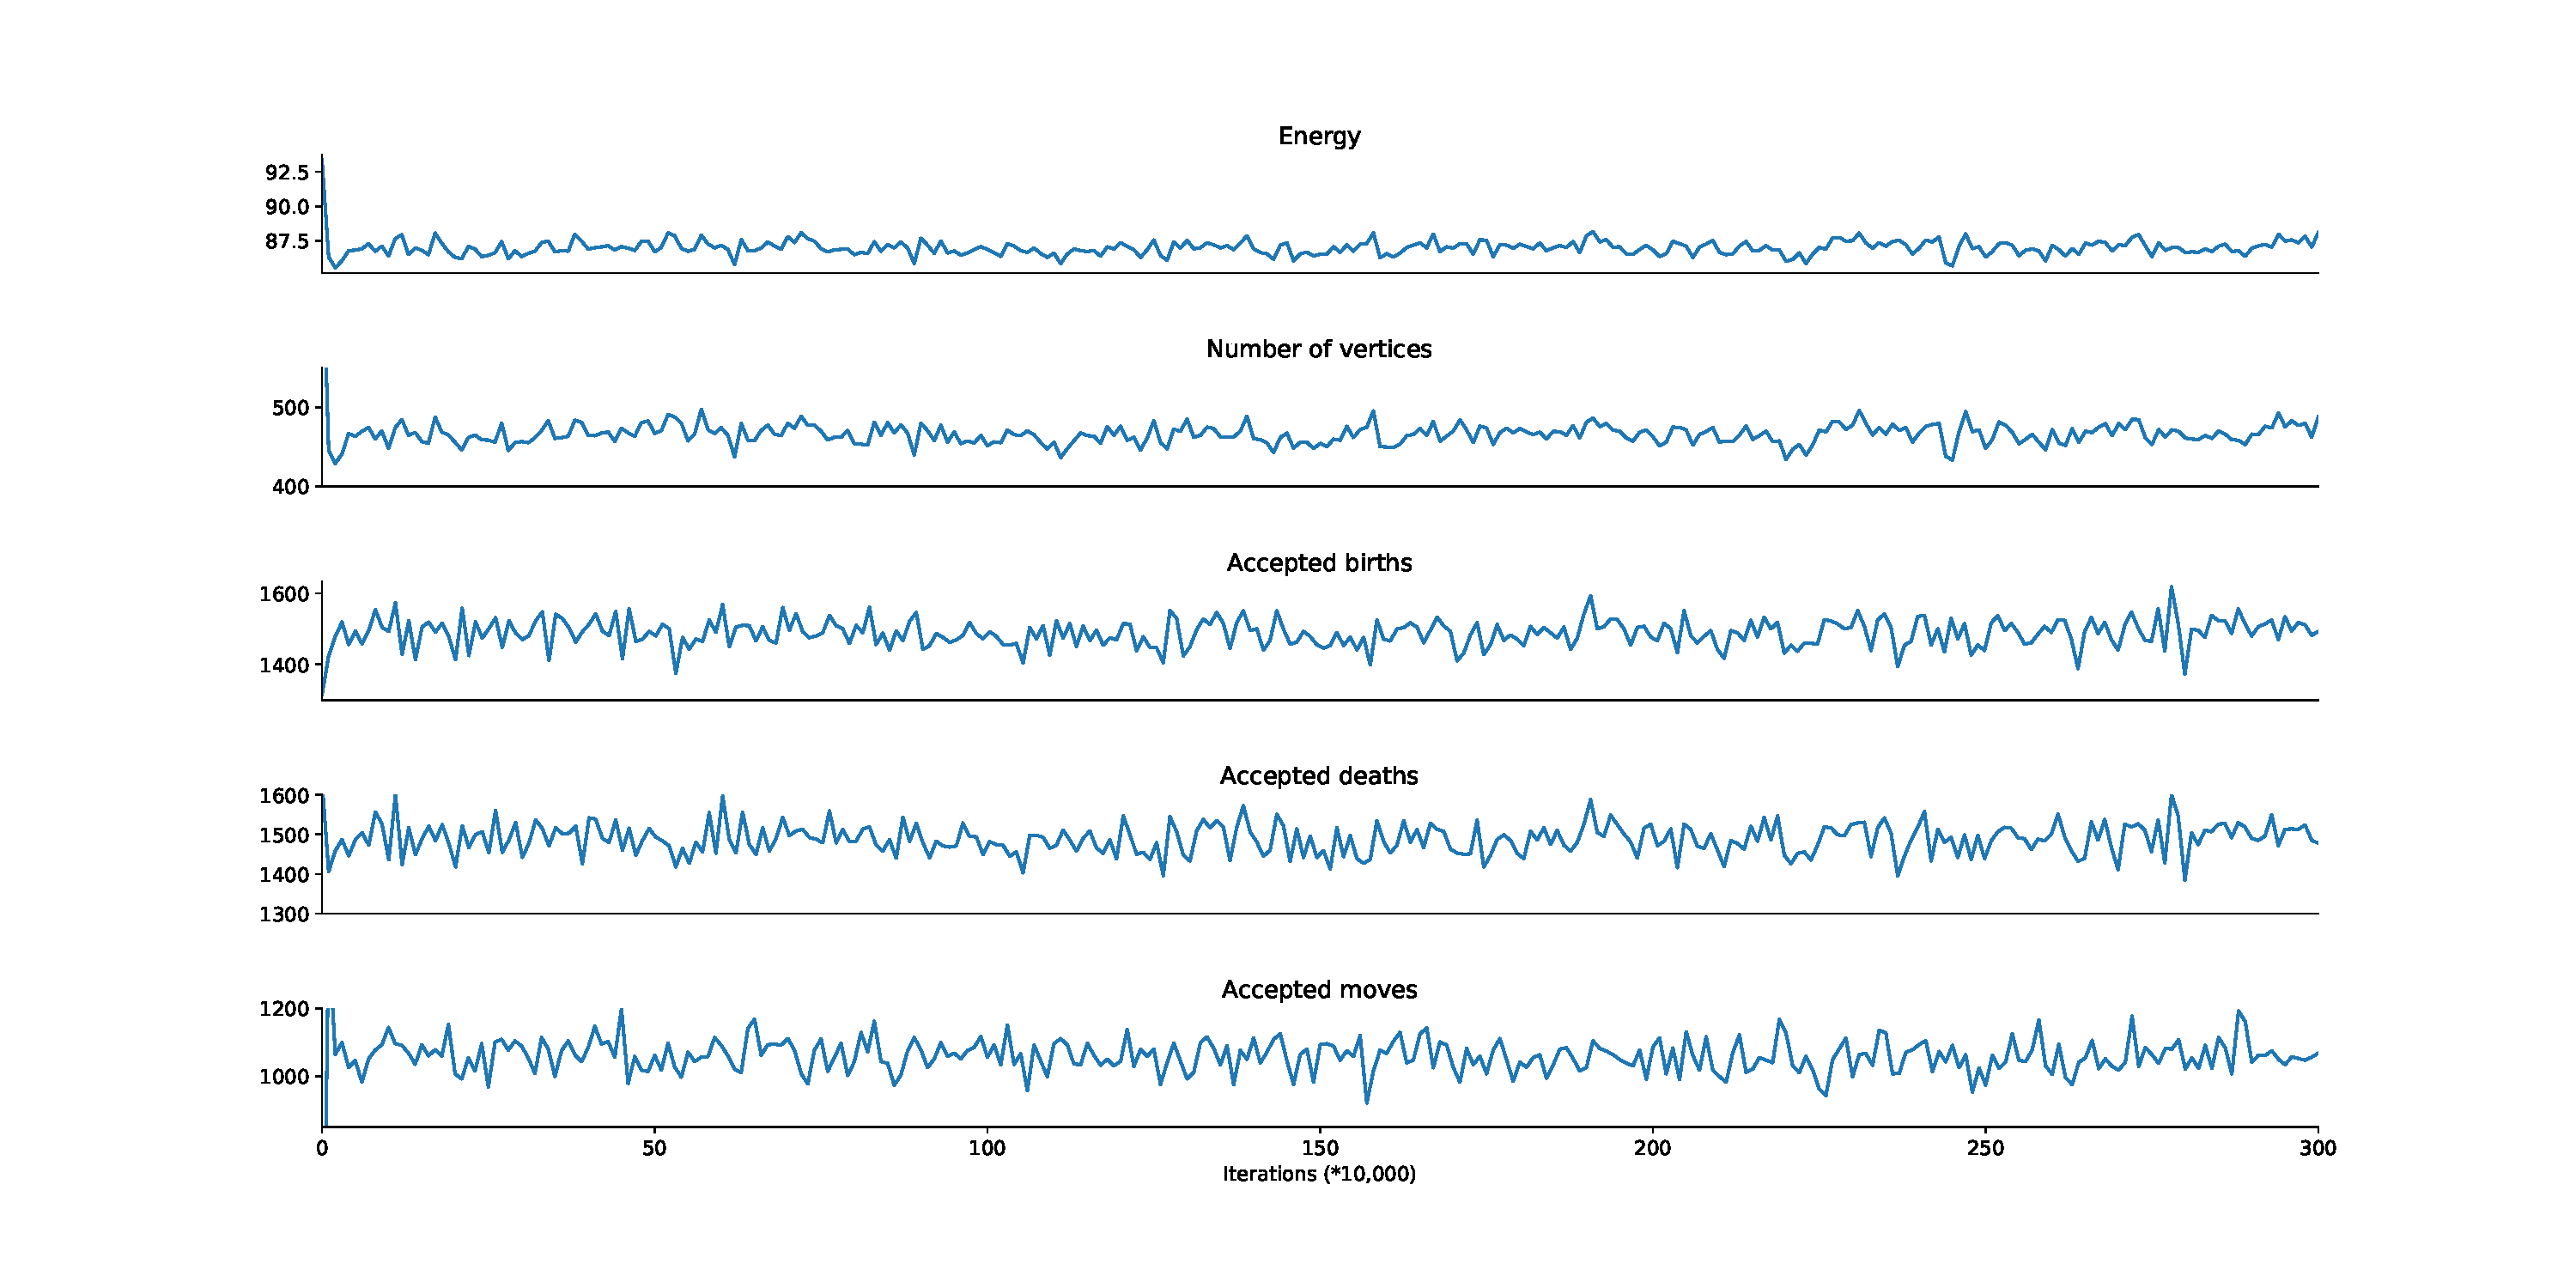
\includegraphics[width=1.3\textwidth]{../img/numeric/convergence.pdf}
  \caption{Convergence metrics for one simulation of \texttt{L+}. Total number of iterations: $3\times 10^6$. $\theta = 1, \alpha = 0.15, z = 500, W = 0.01$.}
  \label{fig:convergence}
\end{figure}




\subsection{Role of $\theta$}
The parameter $\theta$ plays an interesting role in our model. As noted before, the GPP favours configurations with lower energy. In case of the potential $\varphi^{\alpha,\theta}_{HC}$, this the configurations are forced to contain fewer larger tetrahedra in order to minimize the overall surface area. The parameter $\theta$ then controls the strength of this effect. Higher $\theta$ should therefore result in a smaller number of larger tetrahedra. This effect can be seen in Figure \ref{fig:thetaeffect} for one realization of the model $L+$.

\begin{figure}
  \centering
  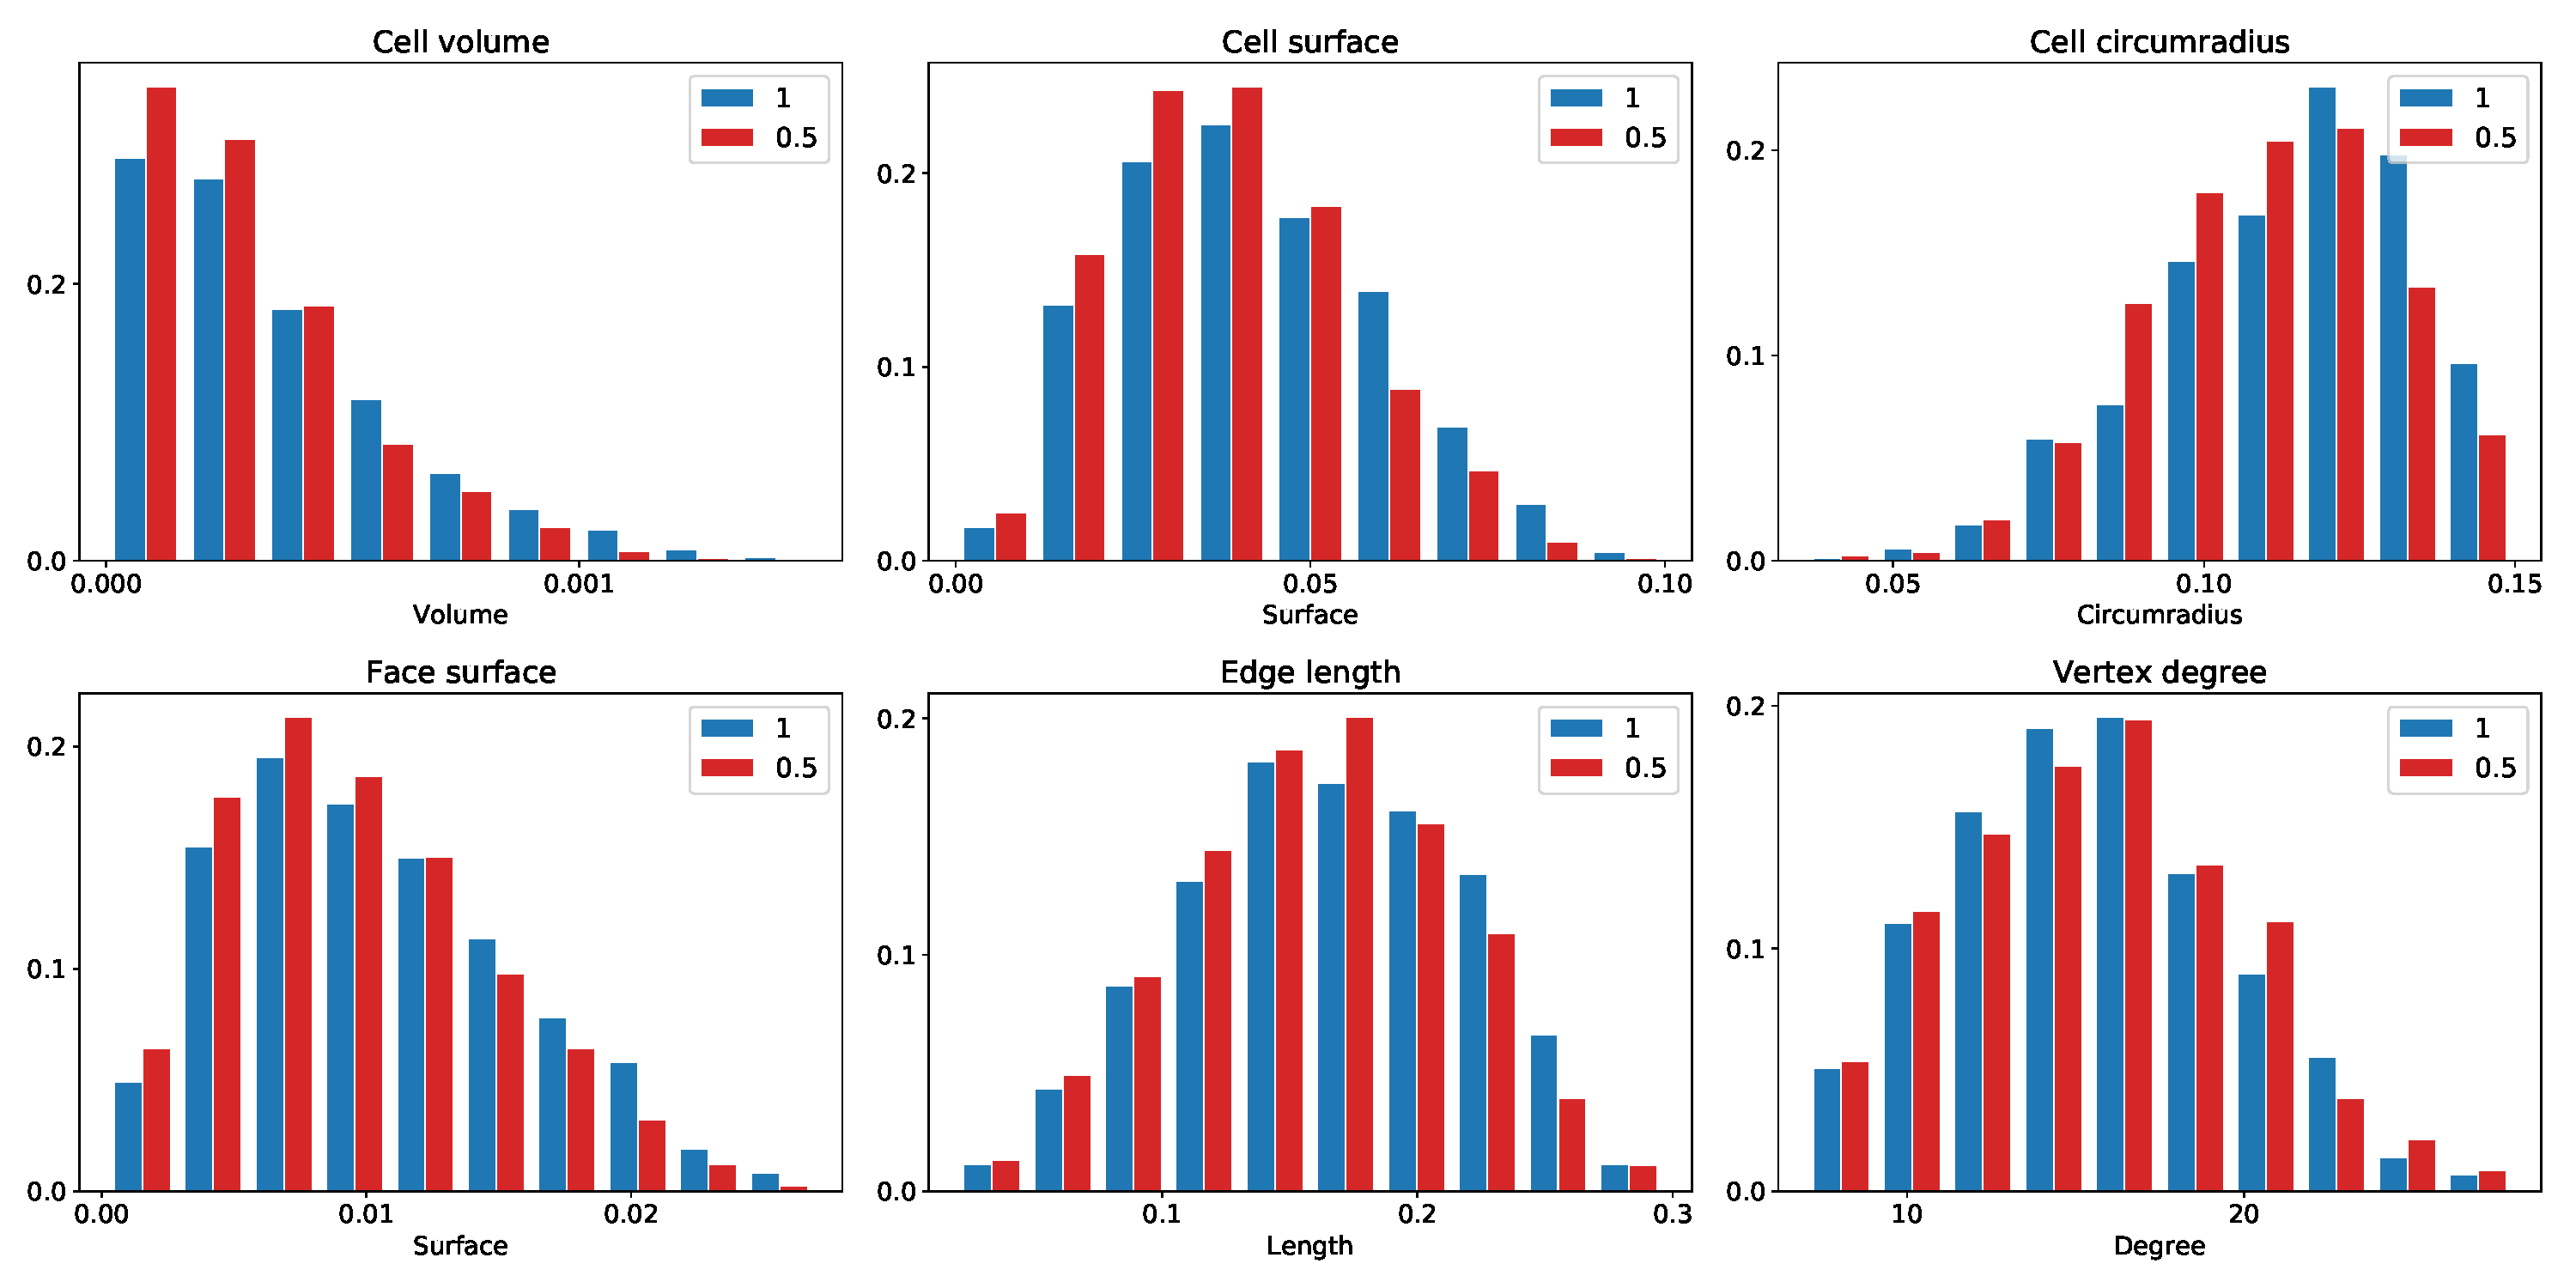
\includegraphics[width=1\textwidth]{../img/numeric/facets_1_05.pdf}
  \caption{Comparison of the distribution of facet statistics for one realization of \texttt{L+} model with $\alpha=0.15,z=500,W=0.01$ and $\theta = 0.5,1$.  }
  \label{fig:thetaeffect}
\end{figure}


Although we have restricted ourselves to the case of non-negative potentials, it is still interesting to attempt to simulate models with a $\theta<0$, even if we do not know whether they exist. Choosing $\theta$ negative reverses the relationship mentioned above. The GPP now favours configurations with greater overall surface area, which should result into a larger number of smaller tetrahedra. This is in fact what happens in the simulation, see Figure \ref{fig:thetanegative}.


% Plot theta pos neg
\begin{figure}
  \centering
    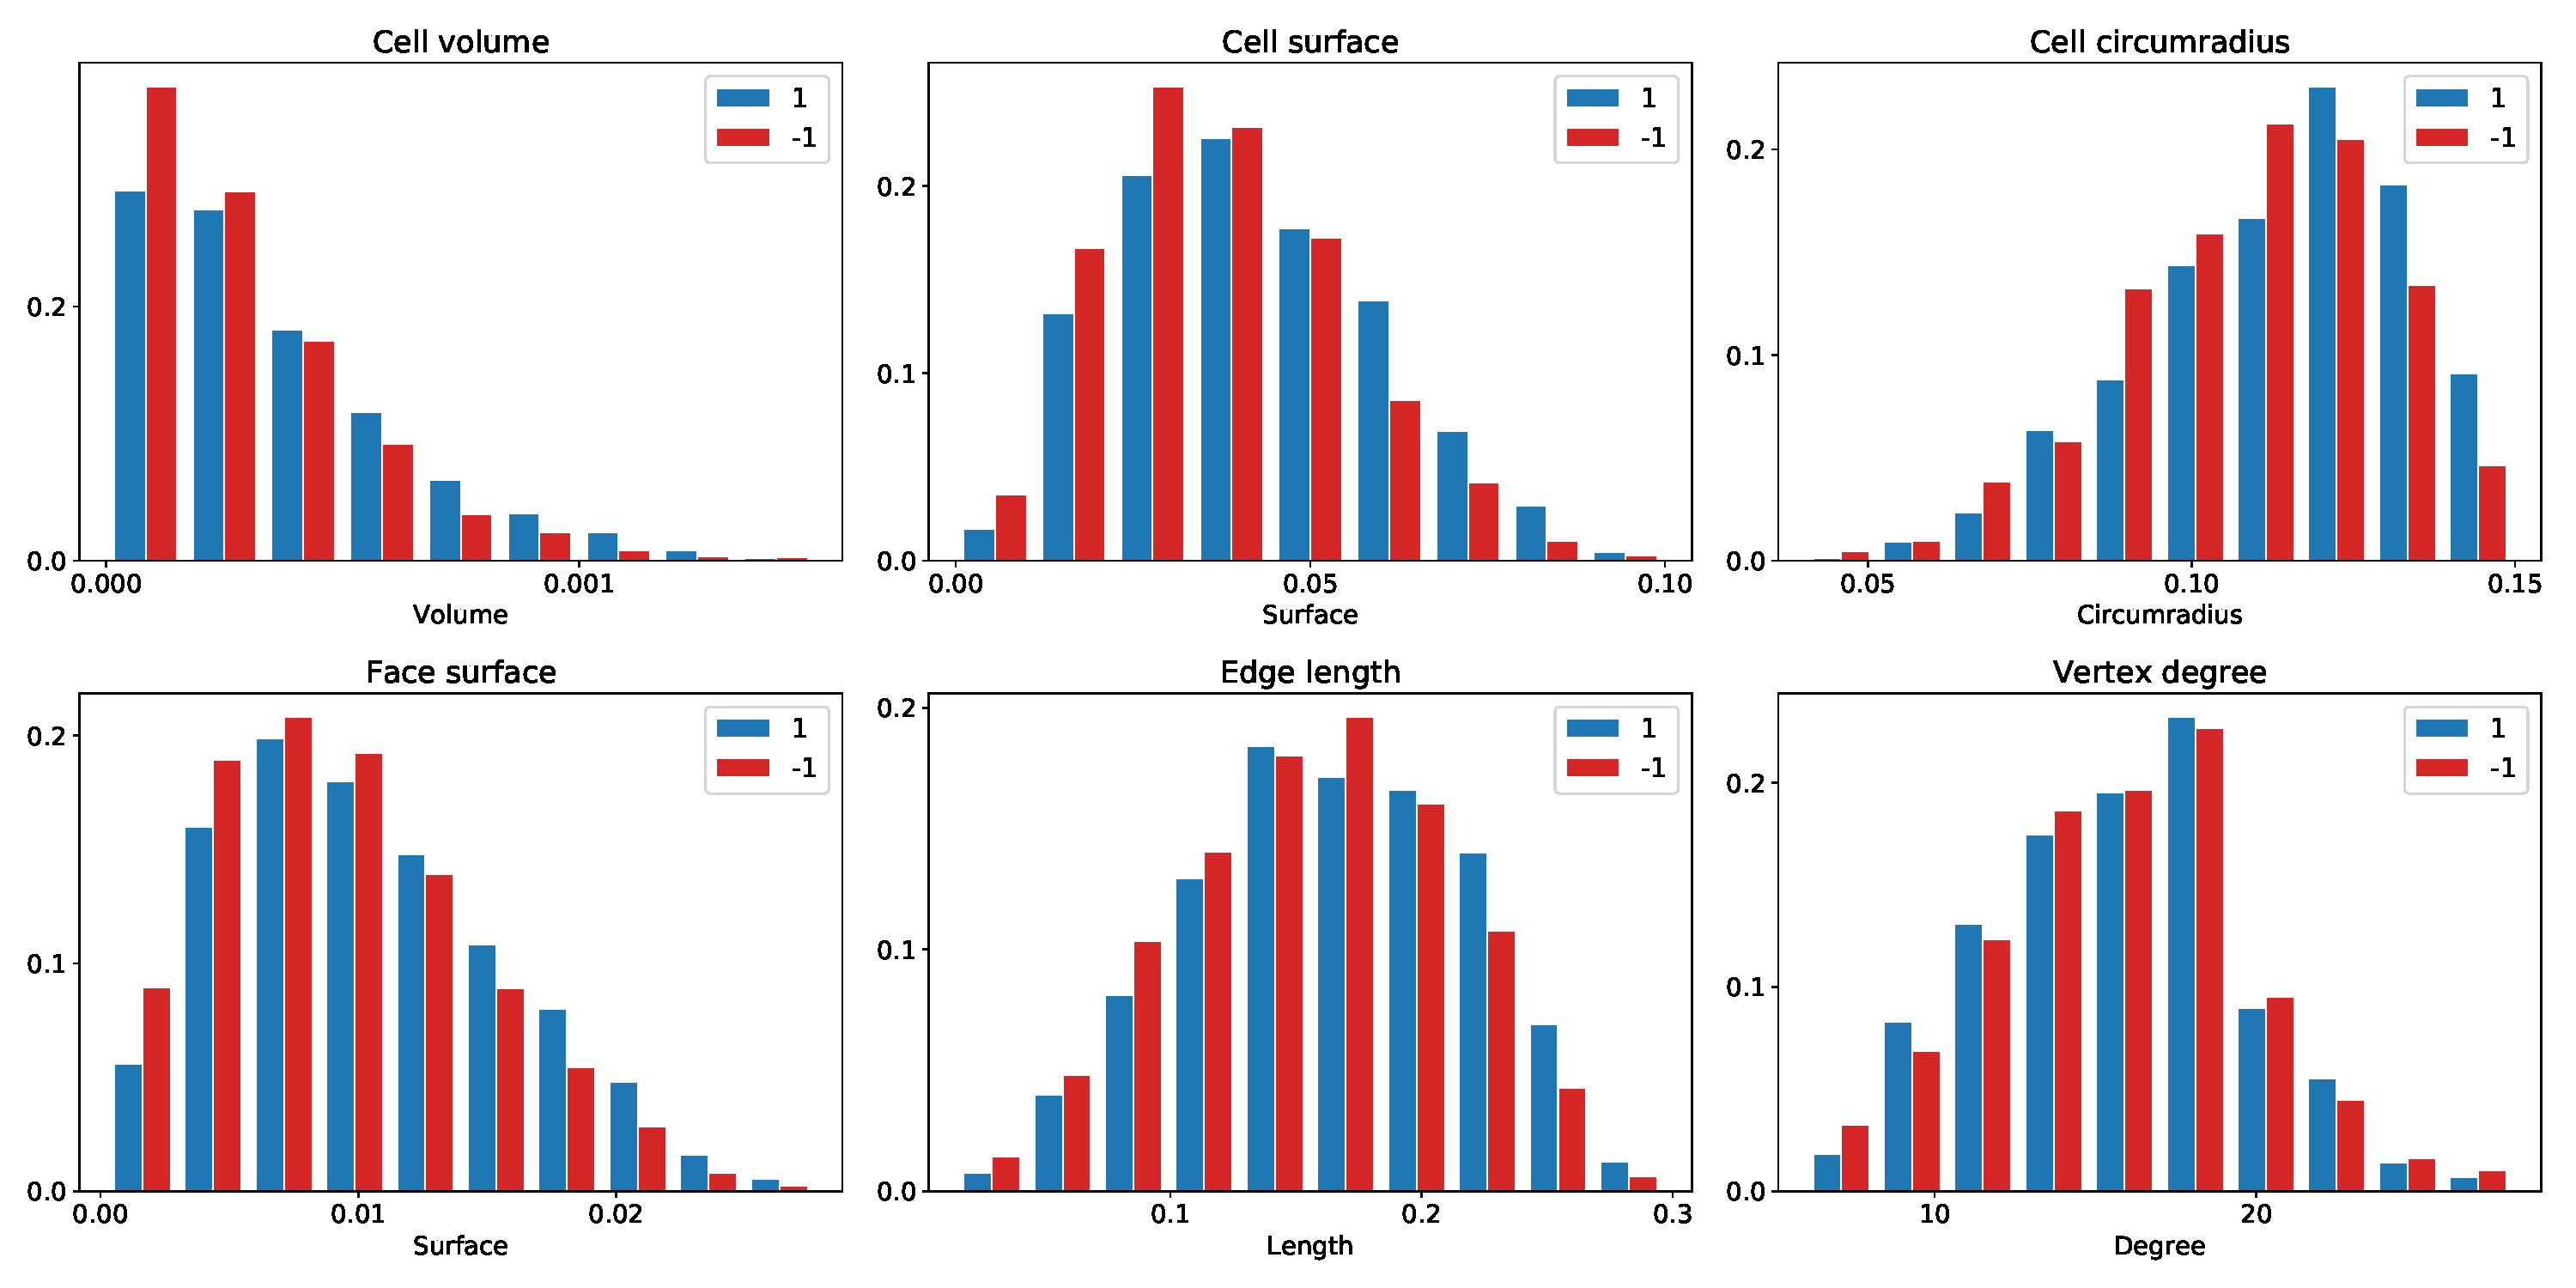
\includegraphics[width=1\textwidth]{../img/numeric/facets_1_-1.pdf}
  \caption{Comparison of the distribution of facet statistics for one realization of \texttt{L+} model with $\alpha=0.15,z=500,W=0.01$ and $\theta = -1,1$.  }
  \label{fig:thetanegative}
\end{figure}




\subsubsection{Obtaining the Poisson tetrahedrization}
\todoo[inline]{This should possibly be shown already in Ch 2 and only referenced here}
From Proposition \ref{prop:poisabscont}, we know that for $\Lambda \in \mathcal B_0(\Rt)$, the Poisson point process with intensity $z$ has the density $f(\gamma)\propto z^{N_\Lambda}(\gamma), \gamma \in \mathbf N_\Lambda$  with respect to $\Pi_\Lambda$. From Definition \ref{def:GPP} of the Gibbs point process we can deduce that if the energy function is zero for all configurations, then the Gibbs point process with activity $z$ reduces to the Poisson point process with intensity $z$.  Figure \ref{fig:PoisvsGibbs} illustrates this point, where the facet distributions of a realization of the model \texttt{L+} with $\theta=0.01$ are compared to the expected values of their counterparts for the Poisson process (found on page $393$ in \cite{Okabe1992}).

% Plot theta 0.01 with Poisson theoretic
\begin{figure}
  \centering
    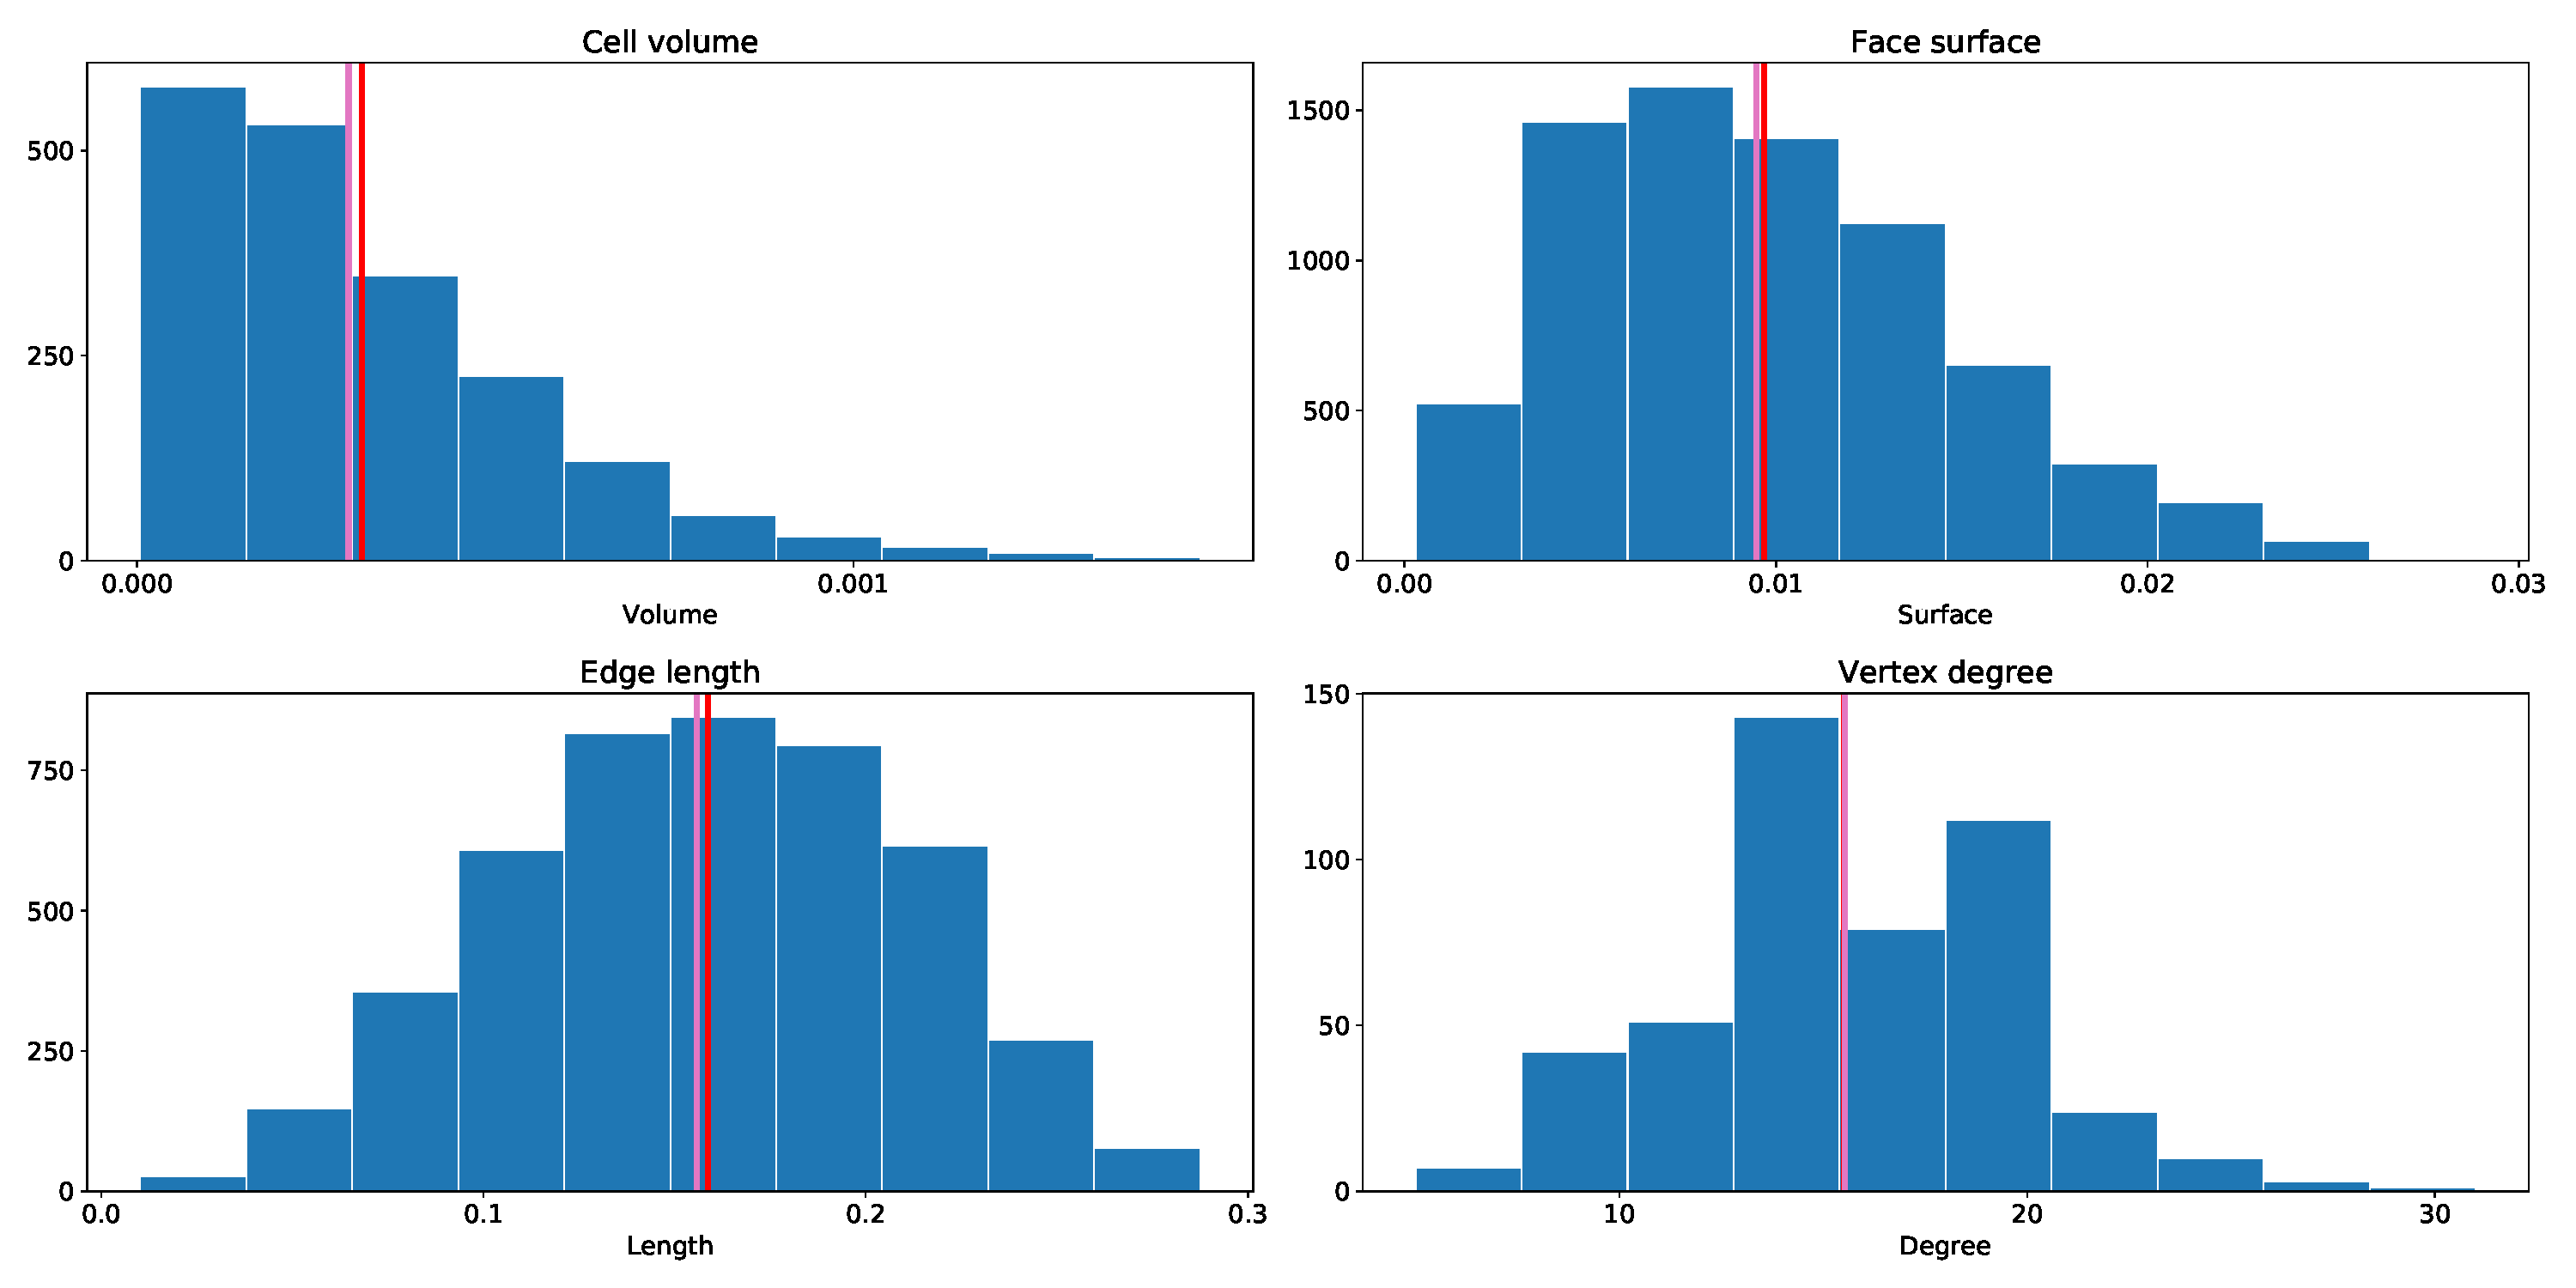
\includegraphics[width=1\textwidth]{../img/numeric/poisson.pdf}
  \caption{Facet distributions of a realization of the \texttt{L+} model with $\alpha=0.15,z=500,W=0.01$ and $\theta = 0.01$. Purple line is the expected value for a Poisson-tetrahedrization, red line is the empirical mean of the realization.  }
  \label{fig:PoisvsGibbs}
\end{figure}




\subsection{Difference between Laguerre and Delaunay}
Perhaps the most interesting comparison to make is between the two models \texttt{D+} and \texttt{L+} with identical parameters. A summary of facet distributions for a realization of both models is shown in Figure  \ref{fig:DelvsLag}.
\todoo[inline]{comment more}

% Plot model differences 

\begin{figure}
  \centering
    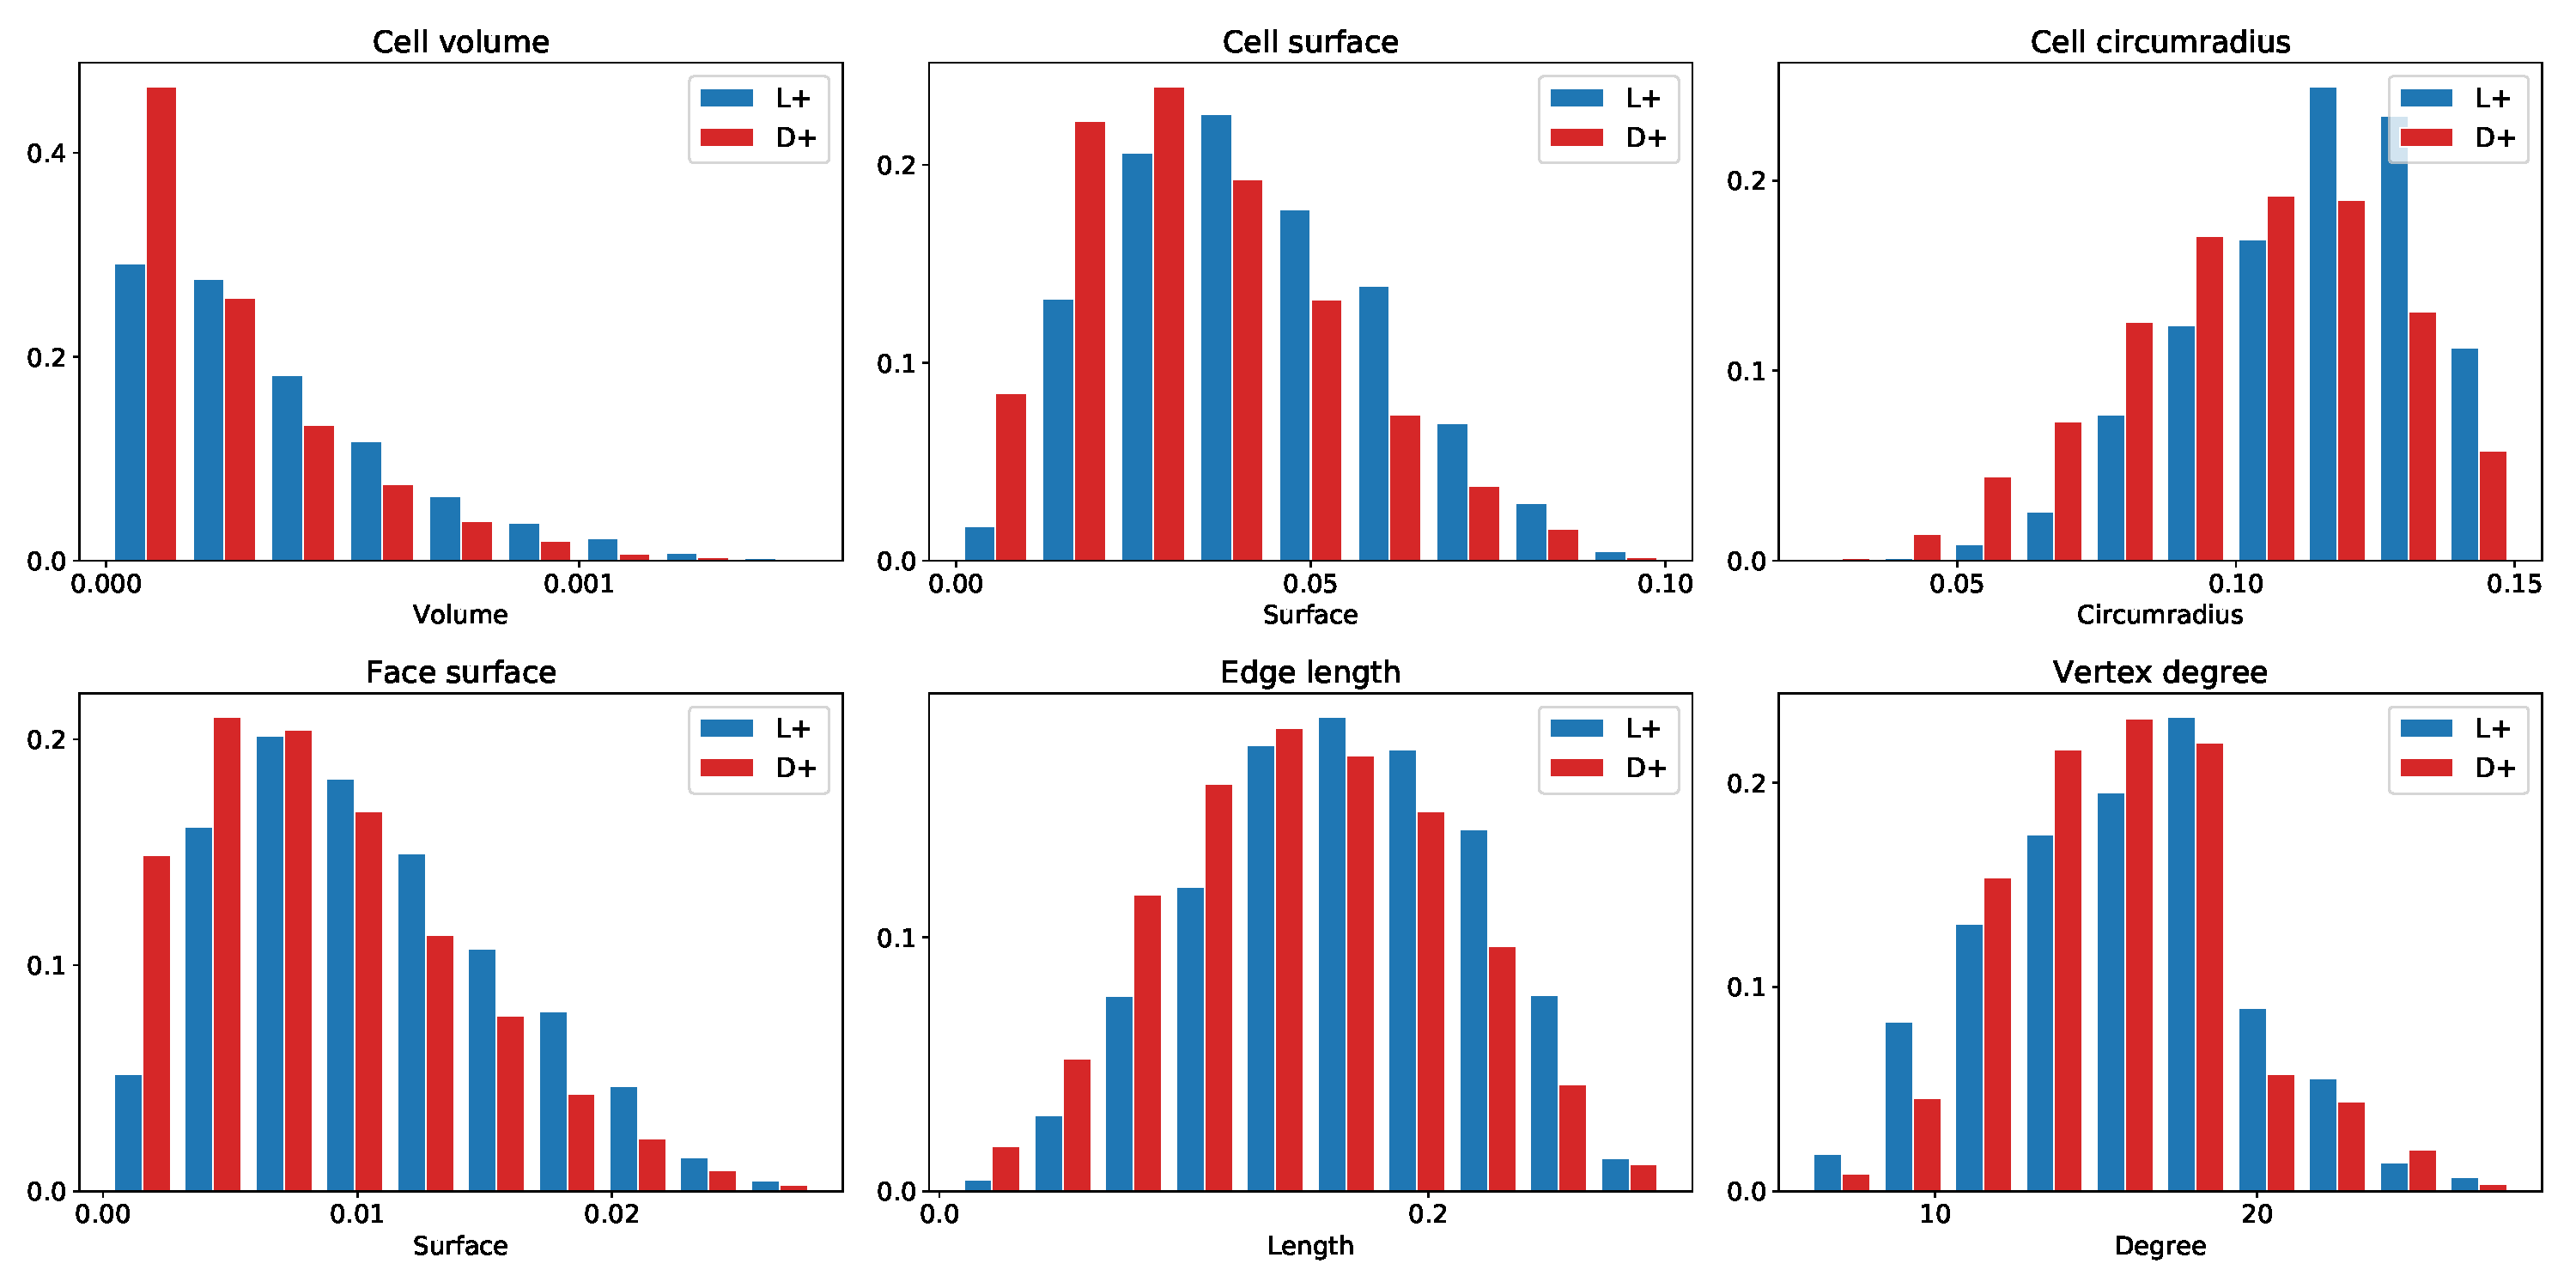
\includegraphics[width=1\textwidth]{../img/numeric/facets_L+_D+.pdf}
  \caption{Facet distribution for a realization of the models \texttt{D+} and \texttt{L+}. Parameters $\theta = 1,\alpha = 0.15, z=500, W=0.01$ for both models.}
  \label{fig:DelvsLag}
\end{figure}


All of the results for both \texttt{D+} and \texttt{L+} with four $\theta$ levels are summarized in Table \ref{tab:facets}, which shows the averages and standard deviations for a $100$ simulations of each model.


\begin{landscape}
\begin{table*}\centering
\ra{1.3}
\begin{tabular}{lrllllllll}\toprule
&& \multicolumn{4}{c}{Cell} & \multicolumn{1}{c}{Face} & \multicolumn{1}{c}{Edge} & \multicolumn{2}{c}{Vertex} \\ 
\cmidrule(lr){3-6} \cmidrule(lr){7-7} \cmidrule(lr){8-8} \cmidrule(lr){9-10}
& Theta &  Count & Volume & Circumradius & Surface & Surface & Length & Count & Degree \\
\midrule
\texttt{D+} \\
 & -1.0 &  2761.3 &  0.00023 &  0.1011 &  0.0322 &  0.0081 &  0.1453 &  639.6 &  15.4 \\
 & &  (108.1) &  (0.00001) &  (0.0012) &  (0.0008) &  (0.0002) &  (0.0017) &  (20.0) &  (0.1) \\
 & -0.5 &  2685.7 &  0.00024 &  0.1015 &  0.0326 &  0.0082 &  0.1461 &  626.2 &  15.4 \\
 & &  (119.9) &  (0.00001) &  (0.0016) &  (0.0010) &  (0.0003) &  (0.0024) &  (22.5) &  (0.1) \\
 & 0.5 &  2509.0 &  0.00025 &  0.1028 &  0.0337 &  0.0085 &  0.1481 &  595.2 &  15.4 \\
 & &  (103.3) &  (0.00001) &  (0.0014) &  (0.0009) &  (0.0002) &  (0.0020) &  (19.0) &  (0.1) \\
 & 1.0 &  2416.4 &  0.00026 &  0.1036 &  0.0344 &  0.0086 &  0.1495 &  577.3 &  15.4 \\
 & &  (100.9) &  (0.00001) &  (0.0013) &  (0.0009) &  (0.0002) &  (0.0018) &  (19.3) &  (0.1) \\
\texttt{L+} \\
 & -1.0 &  2082.9 &  0.00030 &  0.1090 &  0.0373 &  0.0094 &  0.1565 &  496.7 &  15.5 \\
 & &  (81.4) &  (0.00001) &  (0.0013) &  (0.0010) &  (0.0003) &  (0.0020) &  (16.5) &  (0.1) \\
 & -0.5 &  2022.4 &  0.00030 &  0.1096 &  0.0378 &  0.0095 &  0.1574 &  484.4 &  15.5 \\
 & &  (92.7) &  (0.00001) &  (0.0012) &  (0.0009) &  (0.0002) &  (0.0019) &  (18.0) &  (0.1) \\
 & 0.5 &  1909.3 &  0.00032 &  0.1105 &  0.0388 &  0.0097 &  0.1593 &  460.8 &  15.6 \\
 & &  (84.8) &  (0.00002) &  (0.0015) &  (0.0012) &  (0.0003) &  (0.0024) &  (16.1) &  (0.1) \\
 & 1.0 &  1855.3 &  0.00033 &  0.1110 &  0.0394 &  0.0099 &  0.1603 &  451.9 &  15.6 \\
 & &  (86.7) &  (0.00001) &  (0.0013) &  (0.0011) &  (0.0003) &  (0.0020) &  (16.3) &  (0.1) \\
\bottomrule
\end{tabular}
\caption{Facet statistics computed from $100$ realizations of each model and $\theta$ setting. Other parameters were set to $\alpha=0.15, z=500, W=0.01$.}
\label{tab:facets}
\end{table*}
\todoo[inline]{Write more, repeat first row, also std}
\end{landscape}





\section{Estimation}
% Estimation results (table+plot) for a few models
This section presents the results of the estimation procedure presented in Chapter \ref{ch:estimation}. Figures \ref{fig:estD05}, \ref{fig:estD1}, \ref{fig:estL05}, and \ref{fig:estL1} each show the results for the models \texttt{D+} and \texttt{L+}  with $\theta$ equal to $0.5$ and $1$. The bottom-right plot in each figure suggests a linear relationship between the estimates $\hat\theta$ and $\hat z$, a relationship that can be seen in the results of \cite{DereudreLavancier2011} as well.
\todoo[inline]{Comment on the badness, add reference to Dereudre}
Table \ref{tab:estsummary} summarizes all estimation results. 


\begin{table*}
\ra{1.3}
\resizebox{\textwidth}{!}{
\begin{tabular}{lrlllllll}\toprule
&& \multicolumn{1}{c}{$\hat\alpha$}& \multicolumn{2}{c}{$\hat\theta$} & \multicolumn{2}{c}{$\hat z$} & \multicolumn{2}{c}{Vertices} \\ 
 \cmidrule(lr){4-5} \cmidrule(lr){6-7} \cmidrule(lr){8-9} 

& $\theta$ &  &  $z$ unknown & $z$ known & $\theta$ unknown & $\theta$ known & All & Removable  \\
\midrule
\texttt{D+} \\
 & 0.5 &  0.14933 &  1.16643 &  0.22831 &  595.83387 &  564.27343 &  595.24 &  538.37 \\
 &  &  (0.00069) &  (0.94777) &  (0.56386) &  (52.15171) &  (23.55674) &  (18.98) &  (23.18) \\
 & 1.0 &  0.14946 &  1.84958 &  0.83162 &  605.18565 &  564.66566 &  577.32 &  515.81 \\
 &  &  (0.00050) &  (1.03663) &  (0.62494) &  (58.29123) &  (25.83548) &  (19.28) &  (24.94) \\
\texttt{L+} \\
 & 0.5 &  0.15455 &  1.20596 &  4.06347 &  306.40235 &  285.50261 &  460.83 &  269.36 \\
 &  &  (0.02235) &  (1.44752) &  (0.84692) &  (41.40474) &  (16.00663) &  (16.13) &  (15.71) \\
 & 1.0 &  0.15580 &  1.71939 &  4.49746 &  312.60278 &  290.65149 &  451.88 &  261.60 \\
 &  &  (0.04506) &  (1.41497) &  (0.76320) &  (46.78521) &  (18.69764) &  (16.31) &  (17.60) \\
\bottomrule
\end{tabular}}
\caption{Estimation summary. Each $\theta$ was simulated $100$ times. Parameters $\alpha=0.15,z=500, W=0.01$. }
\label{tab:estsummary}
\end{table*}





\begin{figure}
  \centering
  \includegraphics[width=1\textwidth]{"../img/numeric/estimation - type_D+_theta_05"}
  \caption{Estimation results for the model \texttt{D+} with parameters $\theta=0.5,z=500,W=0.01$ for 100 realizations.}
  \label{fig:estD05}
\end{figure}


\begin{figure}
  \centering
  \includegraphics[width=1\textwidth]{"../img/numeric/estimation - type_D+_theta_1"}
  \caption{Estimation results for the model \texttt{D+} with parameters $\theta=1,\alpha=0.15,z=500,W=0.01$ for 100 realizations. Average number of removable points: $442$.}
  \label{fig:estD1}
\end{figure}

\begin{figure}
  \centering
  \includegraphics[width=1\textwidth]{"../img/numeric/estimation - type_L+_theta_05"}
  \caption{Estimation results for the model \texttt{L+} with parameters $\theta=0.5,z=500,W=0.01$ for 100 realizations. }
  \label{fig:estL05}
\end{figure}


\begin{figure}
  \centering
  \includegraphics[width=1\textwidth]{"../img/numeric/estimation - type_L+_theta_1"}
  \caption{Estimation results for the model \texttt{L+} with parameters $\theta=1,\alpha=0.15,z=500,W=0.01$ for 100 realizations. Average number of removable points: $261$.}
  \label{fig:estL1}
\end{figure}






\chapter*{Conclusion}
\addcontentsline{toc}{chapter}{Conclusion}

\todoo[inline]{Summary of what was done}
A considerable number of results is outside the scope of this text, not necessarily because of the difficulty of obtaining them, but simply because of the limited time allotted for its completion. 

The first extentsion would be to complete the results in this text --- that is extend the existing results of \cite{DereudreLavancier2009}  in irreducibility of the Markov chain and \cite{DereudreLavancier2011} in consistency of the MPLE estimates to the three-dimensional Laguerre-Delaunay case. As with existence, it is likely the case that the extension to Laguerre would be easier than the extension to three dimensions. 

Second extension is to study the stability of the potentials without the assumptions of non-negativity. The question, as noted in [ref], depends on the complexity of the tetrahedrization. It seems likely to us that there are relatively easily obtainable results on the complexity of the tetrahedrization of the Poisson process and then perhaps even for the Gibbs point process. Obtaining some results for the tetrahedrization generated by the Poisson process would be interesting in and of itself, as the study of such structures is popular in the field of computational geometry.

A number of other extensions were considered. There are many possibilities in specifying potentials of a different form, in particular studying non-unary potentials by including explicit tetrahedral interactions. This would require new proofs of existence, convergence of MCMC and consistency of the estimation techniques. In the practical sense, it should be relatively easy to extend our \texttt{C++} implementation to include tetrahedral interactions.

Different estimation techniques could be tried. Although we are limited in their choice by the absence of hereditarity, options do exist. One of them is the variational estimator which is applicable even in the non-hereditary case (\cite{BaddeleyDereudre2013}).

In the practical implementation, an interesting comparison would be to try to use the periodic outside configuration as \cite{DereudreLavancier2011} does.

Finally, instead of using the power distance to define the tetrahedrization, we could use a weighted Euclidean metric (\cite{Gavrilova}), resulting in the dual of the so-called Apollonius diagram, or Johnson-Mehl tessellation. 



%%% Bibliography
%%% Bibliography (literature used as a source)
%%%
%%% We employ bibTeX to construct the bibliography. It processes
%%% citations in the text (e.g., the \cite{...} macro) and looks up
%%% relevant entries in the bibliography.bib file.
%%%
%%% The \bibliographystyle command selects, which style will be used
%%% for references from the text. The argument in curly brackets is
%%% the name of the corresponding style file (*.bst). Both styles
%%% mentioned in this template are included in LaTeX distributions.

\bibliographystyle{plainnat}    %% Author (year)
% \bibliographystyle{unsrt}     %% [number]

\renewcommand{\bibname}{Bibliography}

%%% Generate the bibliography. Beware that if you cited no works,
%%% the empty list will be omitted completely.

\bibliography{bibliography}

%%% If case you prefer to write the bibliography manually (without bibTeX),
%%% you can use the following. Please follow the ISO 690 standard and
%%% citation conventions of your field of research.

% \begin{thebibliography}{99}
%
% \bibitem{lamport94}
%   {\sc Lamport,} Leslie.
%   \emph{\LaTeX: A Document Preparation System}.
%   2nd edition.
%   Massachusetts: Addison Wesley, 1994.
%   ISBN 0-201-52983-1.
%
% \end{thebibliography}


%%% Figures used in the thesis (consider if this is needed)
\listoffigures

%%% Tables used in the thesis (consider if this is needed)
%%% In mathematical theses, it could be better to move the list of tables to the beginning of the thesis.
\listoftables

\appendix

\chapter{Appendix: Geometry}\label{appendix}
This appendix investigates some facts and propositions pertaining to geometry in $\mathbb R^3$. Since marked points are not present here, the dashed notation introduced in Chapter \ref{ch:1} will be dropped.

\problem[inline]{This chapter needs better notation. E.g. $S(p_1,p_2,p_3,p_4)$ for a sphere defined by those points, etc.}
\section{Calculating the circumdiameter}
\todoo[inline]{Check circumdiameter x circumradius, it's a bit confusing in many places}
Here we describe how to calculate the circumdiameter of a $3-$simplex through the Cayley-Menger determinant (\cite{Cayley1841}, \cite{Menger28}, \cite{Uspensky48}) \todoo{Improve the references (chapter, placement,..)}~.

First, consider the points $p_1,\dots, p_5 \in \mathbb R^4$ which form a $4$-simplex. Denote $d_{ij} = \|p_i - p_j\|, i,j=1,\dots,5$. Then the area $A$ of the $4-simplex$ is given by the \textbf{Cayley-Menger determinant}[ref sommervile]\todoo[inline]{citation}. 

$$
-9216 A^2 =
\begin{vmatrix}
0 & 1 & 1 & 1 & 1 & 1 \\
1 & 0 & d^2_{12} & d^2_{13} & d^2_{14} & d^2_{15} \\
1 & d^2_{21} & 0 & d^2_{23} & d^2_{24} & d^2_{25}  \\
1 & d^2_{31} & d^2_{32} & 0 & d^2_{34} & d^2_{35} \\ 
1 & d^2_{41} & d^2_{42} & d^2_{43} & 0 & d^2_{45} \\
1 & d^2_{51} & d^2_{52} & d^2_{53} & d^2_{54} & 0 
\end{vmatrix}. 
$$
Now consider non-coplanar points $p_1,\dots, p_4 \in \Rt$ forming a $3$-simplex, i.e. a tetrahedron. To obtain the circumradius of this tetrahedron we imagine $p_1,\dots, p_4$ to lie on a $3$-dimensional hyperplane $H$ in $\mathbb R^4$ and we consider the point $c \in H$ such that $\|c-p_i\| = r$ for all $i=1,\dots,4$, $r\in \mathbb R$. The point $c$ is, by definition, the center of the circumsphere of $p_1,\dots,p_4$ and $r$ is the circumradius. The circumradius $r$ can be obtained using the Cayley-Menger determinant, since $p_1,\dots,p_4,c$ now form a $4$-dimensional simplex of volume $0$. We therefore have 


\begin{equation}\label{eq:CMeq}
0 = 
\begin{vmatrix}
0 & 1 & 1 & 1 & 1 & 1 \\
1 & 0 & d^2_{12} & d^2_{13} & d^2_{14} & r^2 \\
1 & d^2_{21} & 0 & d^2_{23} & d^2_{24} & r^2 \\
1 & d^2_{31} & d^2_{32} & 0 & d^2_{34} & r^2 \\ 
1 & d^2_{41} & d^2_{42} & d^2_{43} & 0 & r^2 \\
1 & r^2 & r^2 & r^2 & r^2 & 0 \\
\end{vmatrix}, 
\end{equation}
where we again have   $d_{ij} = \|p_i - p_j\|, i,j=1,\dots,4$.\newline  

It would be possible to solve \ref{eq:CMeq} as an equation of $r$. A better approach is to  subtract $r^2$ times the first row from last and subtract $r^2$ times the first column from the last to obtain the determinant 



$$
\begin{vmatrix}
0 & 1 & 1 & 1 & 1 & 1 \\
1 & 0 & d^2_{12} & d^2_{13} & d^2_{14} & 0 \\
1 & d^2_{21} & 0 & d^2_{23} & d^2_{24} & 0 \\
1 & d^2_{31} & d^2_{32} & 0 & d^2_{34} & 0 \\ 
1 & d^2_{41} & d^2_{42} & d^2_{43} & 0 & 0 \\
1 & 0 & 0 & 0 & 0 & -2r^2 \\
\end{vmatrix}. 
$$
By expanding by the last row, we obtain the equation

$$
2r^2 \begin{vmatrix}
0 & 1 & 1 & 1 & 1 \\
1 & 0 & d^2_{12} & d^2_{13} & d^2_{14} \\
1 & d^2_{21} & 0 & d^2_{23} & d^2_{24} \\
1 & d^2_{31} & d^2_{32} & 0 & d^2_{34} \\ 
1 & d^2_{41} & d^2_{42} & d^2_{43} & 0 \\
\end{vmatrix} 
-
\begin{vmatrix}
1 & 1 & 1 & 1 & 1 \\
0 & d^2_{12} & d^2_{13} & d^2_{14} & 0 \\
d^2_{21} & 0 & d^2_{23} & d^2_{24} & 0 \\
d^2_{31} & d^2_{32} & 0 & d^2_{34} & 0 \\ 
d^2_{41} & d^2_{42} & d^2_{43} & 0 & 0 \\
\end{vmatrix} = 0,
$$
from which $r^2$ is directly expressible as

\begin{equation}\label{eq:Cayley-Menger-expanded}
r^2 
=
\frac{
\begin{vmatrix}
1 & 1 & 1 & 1 & 1 \\
0 & d^2_{12} & d^2_{13} & d^2_{14} & 0 \\
d^2_{21} & 0 & d^2_{23} & d^2_{24} & 0 \\
d^2_{31} & d^2_{32} & 0 & d^2_{34} & 0 \\ 
d^2_{41} & d^2_{42} & d^2_{43} & 0 & 0 \\
\end{vmatrix}}
{2 \begin{vmatrix}
0 & 1 & 1 & 1 & 1 \\
1 & 0 & d^2_{12} & d^2_{13} & d^2_{14} \\
1 & d^2_{21} & 0 & d^2_{23} & d^2_{24} \\
1 & d^2_{31} & d^2_{32} & 0 & d^2_{34} \\ 
1 & d^2_{41} & d^2_{42} & d^2_{43} & 0 \\
\end{vmatrix} 
}.
\end{equation}
It is worth noting that the determinant in the quotient cannot equal zero, since it is again a Cayley-Menger determinant and we assumed $p_1,\dots,p_4$ to be non-coplanar. 



\section{Bounding the circumdiameter}\label{sec:boundingdiameter}
\todoo[inline]{Say a bit more about what this is}
This section derives the bounds used in Theorems \ref{thm:E1}, \ref{thm:E2}, \ref{thm:E3}, \ref{thm:E4}, and Propositions \ref{prop:maxcircum} and \ref{prop:maxPeta}. 

\subsection{Statement of the problem}
The problem of founding the bounds can be stated as the following two optimization problems. \newline

\noindent For the tetrahedron $T_1$, the problem is 
\begin{equation}\label{prob:tetra1}
\begin{aligned}
& \underset{p_1,p_2,p_3,p_4\in \Rt}{\text{maximize}}
& & \delta(\{p_1,p_2,p_3,p_4\}) \\
& \text{subject to}
& & \| p_i - t_i\| \leq \rho a, t_i\in \Rt, i=1,2,3,4, \\
& & &\|t_i - t_j\| = a, i=1,2,3,4. 
\end{aligned}
\end{equation}

\noindent To state the problem for the tetrahedron $T_2$, first denote 
$$D = \begin{pmatrix}
0 & \sqrt 2  a & a & a \\
\sqrt 2 a & 0 & a & a \\
a & a & 0 & a\\
a & a & a & 0
\end{pmatrix},
$$
and denote the entries of matrix $D$ as $d_{ij}, i,j=1,2,3,4$. Then the statement is:
\begin{equation}\label{prob:tetra2}
\begin{aligned}
& \underset{p_1,p_2,p_3,p_4\in \Rt}{\text{maximize}}
& & \delta(\{p_1,p_2,p_3,p_4\}) \\
& \text{subject to}
& & \|p_i - t_i\| \leq \rho a, t_i\in \Rt, i=1,2,3,4, \\
& & & \|t_i-t_j\| = d_{ij}, i,j=1,2,3,4.\\
\end{aligned}
\end{equation}
This is a non-linear optimization problem. We can arrive at its solution through some careful geometric arguments.

\subsection{Solution to the problem}
First, define the \textit{circumdiameter function} of point $p \in \Rt$ with respect to non-collinear points $p_1,p_2,p_3 \in \Rt$:
$$c(p) = \delta(\{p,p_1,p_2,p_3\}).$$
Denote $(x_i,y_i,z_i)$ the coordinates of $p_i, i=1,\dots,3$. Denote $\delta(\{p_1,p_2,p_3\})$ the circumdiameter of the triangle formed by $p_1,p_2,p_3$. The following lemma describes the properties of $c(p)$.

\begin{lemma} $c(p)$ is continuous, has a global minimum $c_{min} := \delta(\{p_1,p_2,p_3\})$ and level sets 
	$$L_a := \{p \in \Rt: c(p)=a\} = S_{a1} \cup S_{a2}, \quad a \geq c_{min},$$ 
	where $S_{a1}$ and $S_{a2}$ are two spheres with diameter $a$ such that $p_1,p_2,p_3 \in S_{a1}\cap S_{a2}$. Furthermore, the centers $c_1, c_2$ of $S_{a1},S_{a2}$ respectively, lie \todoo{Improve the wording}in the halfspaces
$$H_+ = \{x \in \Rt: Ax \geq 0 \},\; H_- = \{x \in \Rt: Ax \leq 0\},$$
where $A$ defines the hyperplane $H=\{x\in\Rt: Ax = 0\}$ on which $p_1,p_2,p_3$ lie.
\end{lemma}
\begin{proof}
	Continuity: From \ref{eq:Cayley-Menger-expanded} we see that $c(p)$ can be seen as a composition of a norm, determinants and division. Determinant is continuous as a function of elements of the matrix since it is a polynomial function. Thus $c(p)$ is continuous.\newline

\noindent We can rewrite $L_a$ as
$$\{p \in \Rt: \exists \text{ sphere } S \text{ s.t. } p_1,p_2,p_3,p \in S \text{ and diam}S = a\}.$$
We must therefore find the number of spheres going through the points $p_1,p_2,p_3$ with the diameter $a$. Denote $S$ a sphere such that $\{p_1,p_2,p_3\}\subset S$ with $\mathrm{diam}(S)=a$. Define the hyperplanes
$$H_{12} = \{x\in\Rt: \|x-p_1\| = \|x-p_2\|\}, \;\; H_{23} = \{x\in\Rt: \|x-p_2\|=\|x-p_3\|\}.$$
The intersection $H_{12}\cap H_{23}$ is a line $L$, as $p_1,p_2,p_3$ are non-collinear.  The center of $S$ is at distance $a/2$ from all three points and thus lies on $L$. For any point, there are at most two points on the line $L$ at a given distance from the point. This proves that there are at most two spheres satisfying the definition of $S$.

Using the line $L$, we can also deduce the rest of the proposition. The point on $L$ at a minimum distance to $p_1,p_2,p_3$ is the point $p_{min}:=L\cap H$. We know that $p_{min}$ is equidistant from $p_1,p_2,p_3$ and that it lies on the hyperplane $H$, therefore it is the circumradius of the triangle defined by $p_1,p_2,p_3$ and we have $c(p_{min}) = \delta(\{p_1,p_2,p_3\})$.  

\todoo[inline]{If possible, simplify this argument}
To see that $c_1$ and $c_2$ must be (non-strictly) separated by the hyperplane $H$, assume without loss of generality $\{c_1,c_2\}\subset H_+, c_1\neq c_2$. Let $p \in S_{a1}$ and let  $p_R\in \Rt$ be the reflection of $p$ through the hyperplane $H$. The tetrahedron $p_1,p_2,p_3,p_R$ then is a reflection of the tetrahedron $p_1,p_2,\dots, p$ and therefore its circumsphere has diameter $a$. However, its centre lies in $H_-$, which is a contradiction. 
\end{proof}

Note that $S_{a1}$ and $S_{a2}$ are not necessarily distinct. In fact, we can see from the proof that $S_{a1}=S_{a2}$ precisely when $a=c_{min}$.


We are now ready to characterize the set of solutions to \ref{prob:tetra1} and \ref{prob:tetra2}. For the next proposition, we say a point lies ``inside'' or ``outside'' of the sphere $S$ if the point lies in $B$ or in $B^c$ respectively, where $B$ is the closed ball such that $\partial B = S$. For the next proposition, define $S(q_1,q_2,q_3,q_4)$ to be the sphere on which $q_1,q_2,q_3,q_4\in\Rt$ lie.


\begin{proposition}\label{prop:ApolloniusSet}
Any solution $(p_1,p_2,p_3,p_4)$ of the problem \ref{prob:tetra1} will lie on a sphere $S$ that is (internally or externally) tangent to the spheres $\partial B(t_i,\rho a), i =1,2,3,4$. 
\end{proposition}
\begin{proof}
	Let $(p_1,p_2,p_3,p_4)$ be a solution of \ref{prob:tetra1}. Denote $c(p_1)=\delta(\{p_1,p_2,p_3,p_4\})=c$ and $S$ the circumsphere of $\{p_1,\dots,p_4\}\subset S$. 
	First, without loss of generality assume that $p_1 \in B(t_1,\rho a)$. Because $p_1$ maximizes the function $c(p)$, we have $c(p_1)\geq c(p), p\in U$, where $U$ is some small neighborhood of $p_1$. Choose two points, $p_O,p_I\in U\setminus S$ such that 
\begin{enumerate} 
\item $c(p_O)=c(p_I)=b$,
\item $p_I$ is on the inside of $S$ and $p_0$ on the outside of $S$ 
\item \todoo{Define this notation}$S(p_I,p_2,p_3,p_4)$ and $S(p_O,p_2,p_3,p_4)$ do not equal and their centers lie on the same halfspace ($H_+$ or $H_-$) as $S$. 
\end{enumerate}
Such choice is possible due to continuity of $c(p)$. Yet we arrive at a contradiction, as the level set $L_b$ now contains two distinct spheres with centres in the same halfspace. 

Assume now that $p_1 \in \partial B(t_1,\rho a)=: S_1$. We now choose $p_I$ and $p_O$ with the additional requirement that they must both lie on $\partial B(t_1,\rho a)$. Such choice is not possible precisely when $S_1$ and $S$ are tangent, since then  $S_1$ lies either completely inside or outside $S$ and it is no longer possible to choose points both outside and inside. 
\end{proof}
\unsure{Is this a good way of proceeding?}Note that Proposition \ref{prop:ApolloniusSet} is formulated for problem \ref{prob:tetra1}. However, we could repeat the same exact argument for \ref{prob:tetra2} and thus the same holds for both problems.\newline

We have found that the solutions to \ref{prob:tetra1} and \ref{prob:tetra2} must lie on a sphere that tangent to the spheres within which points can move. This is a dramatic improvement --- we have narrowed the previously infinite space of possible solutions down to just $2^4=16$ possible quadruples of points (and even less because of symmetries). We also note that the set of solutions to our problem is precisely the set of solutions of a three-dimensional equivalent of the more than two thousand years old \todoo{Encoding problem} \textbf{Apollonius problem} 
% \cite{GischRibando2006}.


\subsection{Apollonius problem in $\mathbb R^3$}
We want to find all the spheres that are externally or internally tangent to the spheres $\partial B(t_i,\rho a), i=2,3,4$ as defined in problems \ref{prob:tetra1} and \ref{prob:tetra2}.

First note that two externally tangent spheres $S_1=((x_1,y_1,z_1),r_1), S_2=((x_2,y_2,z_2),r_2)$  satisfy
$$\|(x_1,y_1,z_1) - (x_2,y_2,z_2)\| = r_1+r_2.$$
Similarly, two externally tangent spheres satisfy
$$\|(x_1,y_1,z_1) - (x_2,y_2,z_2)\| = |r_1 - r_2|.$$
By squaring both equations, we obtain the equality
$$(x_1-x_2)^2 + (y_1-y_2)^2 + (z_1-z_2)^2 = (r_1 \pm r_2)^2$$
Where we use $+$ for externally and $-$ for internally tangent spheres.

The Apollonius problem for spheres $S_1,S_2,S_3,S_4$ is therefore solved by any $S=((x,y,z),r)$ such that
\begin{align}\label{eq:Apollonius}
  (x_1-x)^2 + (y_1-y)^2 + (z_1-z)^2 &= (r_1 \pm r)^2 \\
  (x_2-x)^2 + (y_2-y)^2 + (z_2-z)^2 &= (r_2 \pm r)^2 \nonumber \\
  (x_3-x)^2 + (y_3-y)^2 + (z_3-z)^2 &= (r_3 \pm r)^2 \nonumber \\
  (x_4-x)^2 + (y_4-y)^2 + (z_4-z)^2 &= (r_4 \pm r)^2, \nonumber  
\end{align}

where we can take any combination of $+$ or $-$, yielding altogether $16$ possible solutions. We do not consider degenerate cases as they cannot happen in our setting. 

As noted previously, the number of solutions for both $T_1$ and $T_2$ will reduce significantly. For $T_1$, the spheres are completely interchangeable and thus only solutions with different number of $+$ will differ. This yields $5$ possible solutions. Geometrically the number of $+$ can be seen as the number of spheres the solution is externally tangent to. For $T_2$ the situation is more complex, as the problem isn't entirely symmetric with respect to the four points. Still, symmetries do exist and the number of solution will be reduced.  

Sadly, for most choices of $+$ and $-$, these equations still seem to be too complex for Mathematica to solve. Luckily, we can simplify them further. 

\subsubsection{Solving the equations \eqref{eq:Apollonius} by linearising}

We formulate the solution as a theorem.
\begin{theorem}\label{thm:Apollonius}
	For $\rho < 1/(2\sqrt 6)$, the maximum in \ref{prob:tetra1} is $a \delta_1$, where
	$$\delta_1 := 2(\sqrt 6/4 + \rho).$$
	For $\rho < 1/4$, the maximum in \ref{prob:tetra2} is $a \delta_2$, where
	$$\delta_2 := 2 \frac{2\rho + \sqrt{2 - 32\rho^2 + 64 \rho^4}}{2-32\rho^2}.$$

\end{theorem}
\begin{proof}
	Recall that the solution must lie on a sphere solving the equations \eqref{eq:Apollonius}. We must therefore solve them and find the solution with the largest circumdiameter.

First, for clarity, we define the variables $s_i\in\{+1,-1\},i=1,\dots,4$ instead of relying on the notation $\pm$. We begin by expanding the parentheses to obtain the equations
$$x^2+y^2+z^2 + x_i^2 + y_i^2 + z_i^2 - 2xx_i - 2yy_i - 2zz_i = r^2 + r_i^2 + 2(s_1 r_1 - s_2 r_2)r,\quad i=1,2,3,4$$

By subtracting the $2,3,4$th equation from the first, we get rid of the quadratic terms and obtain a system of linear equations with four variables and three equations:
\begin{align*}-&2(x_1-x_i)x - 2(y_1-y_i)y -2 (z_1-z_i)z - 2(s_1r_1 - s_2r_2)r \\
	& + x_1^2-x_i^2 + y_1^2-y_i^2 + z_1^2 - z_i^2 -r_1^2 + r_i^2 = 0, \quad i=2,3,4
\end{align*}
This system can be solved to obtain expression of $x,y,z$ in terms of $r$. We then substitute those expression into \eqref{eq:Apollonius} to obtain $r$\footnote{Note that exact solutions of $x,y,z$, which we are not interested in, could then by obtained through substituting $r$ back into the linear system.}. 

We have used Wolfram Mathematica \cite{Mathematica} to find the solutions. The full implementation can be found in the file \texttt{ApolloniusProblem.nb}. By comparing the circumdiameters of the solutions, we obtain the proposition.

\end{proof}
All the solutions for the choice $a=1$ can be seen in Figures \ref{fig:Apollonius1} and \ref{fig:Apollonius2}. We can see that for $T_1, \rho < 1/\sqrt 6$, we have the two solutions
$$a(\sqrt 6 / 4 + \rho), a \frac{\rho - \sqrt 6 (4\rho^2 - 1)}{4-24 \rho^2}$$
which intersect at $\rho =1/(2\sqrt 6)$. 

Notice the simple linear form of the first solution --- it is precisely the sphere which is internally tangent to all four spheres. This sphere has the same center as the circumsphere of tetrahedron $\{t_1,t_2,t_3,t_4\}$. Thus the solution is a sum of circumradius of the tetrahedron, $\sqrt 6 /4$, and the radius of the four spheres, $\rho$. We can see similar behaviour in the solution that is externally tangent to all four spheres.

For $T_2$, the linear solution will no longer be the largest, as now we obtain a larger circumradius by using a sphere that is externally tangent to some of the spheres. 


\begin{remark}\label{rem:GP}[General position]
	From the form of the solutions one can also obtain the necessary bounds for $\rho$ for the points to remain in general position. The points cease to be in general position precisely when any one of the solutions becomes infinite. This gives us $\rho < 1/(2\sqrt 6)$ for $T_1$ and $\rho<1/4$ for $T_2$. Since we must control the circumdiameter for all tetrahedra, we must assume $\rho < 1/4$.
\end{remark}


\begin{figure}
	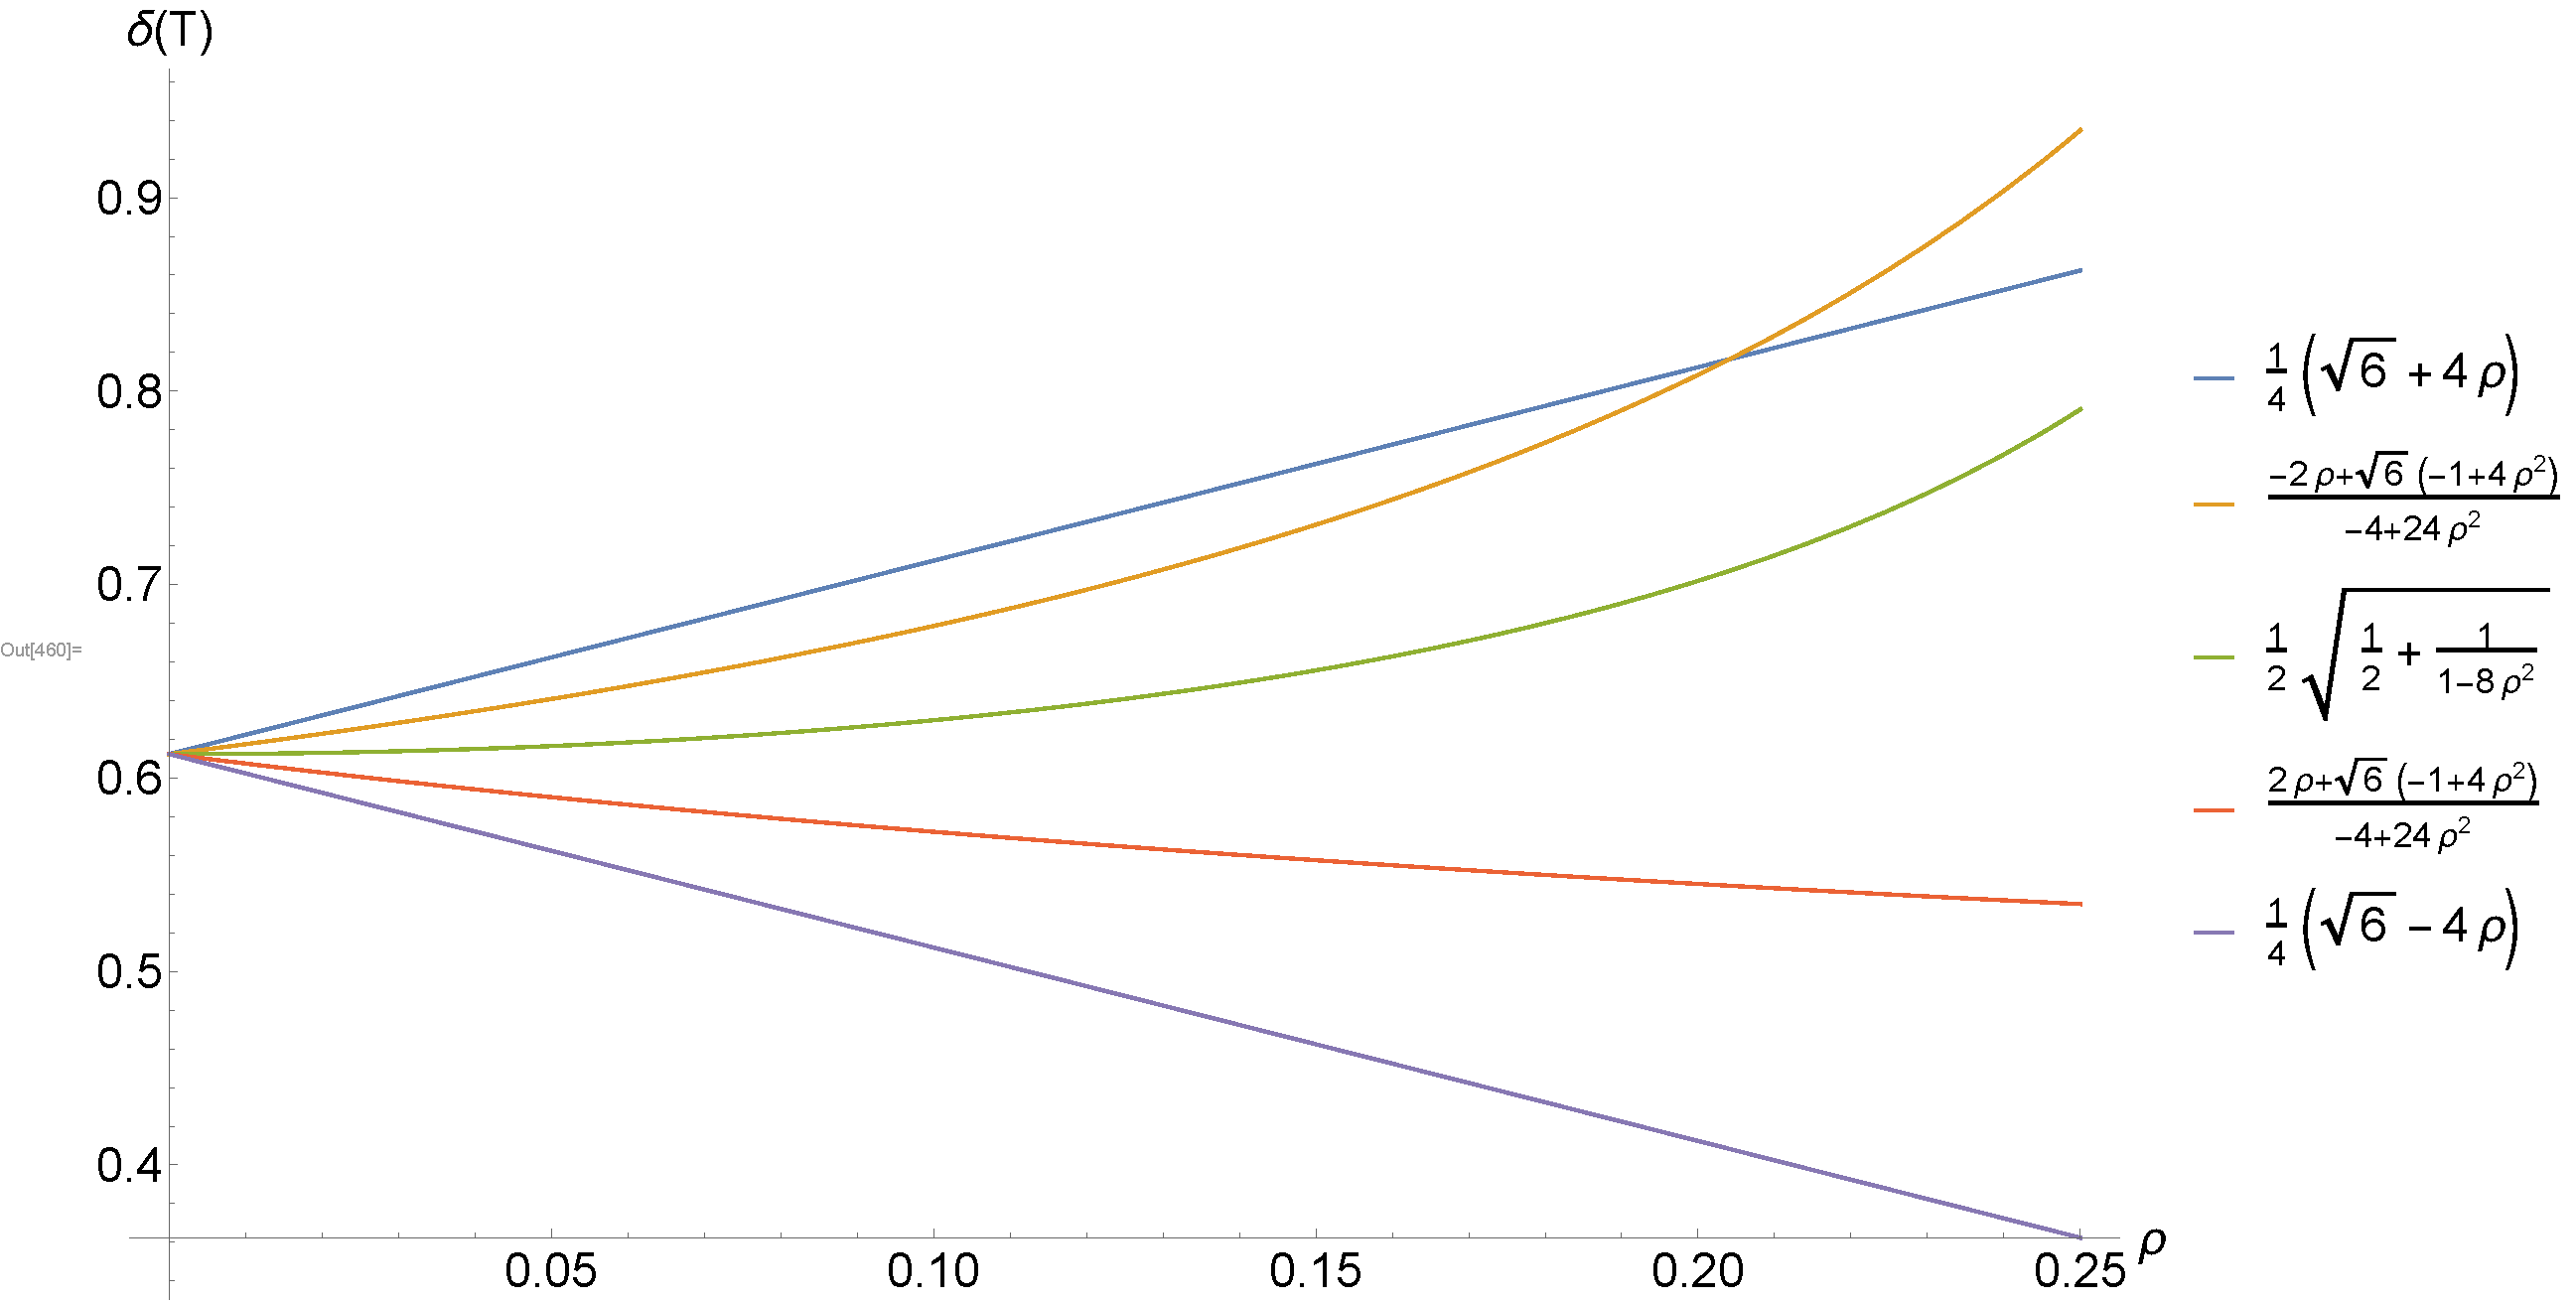
\includegraphics[width=1\textwidth]{../img/t1.pdf}
	\caption{All solutions to Apollonius problem with $T_1$, $a=1$.}\label{fig:Apollonius1}
\end{figure}

\begin{figure}
	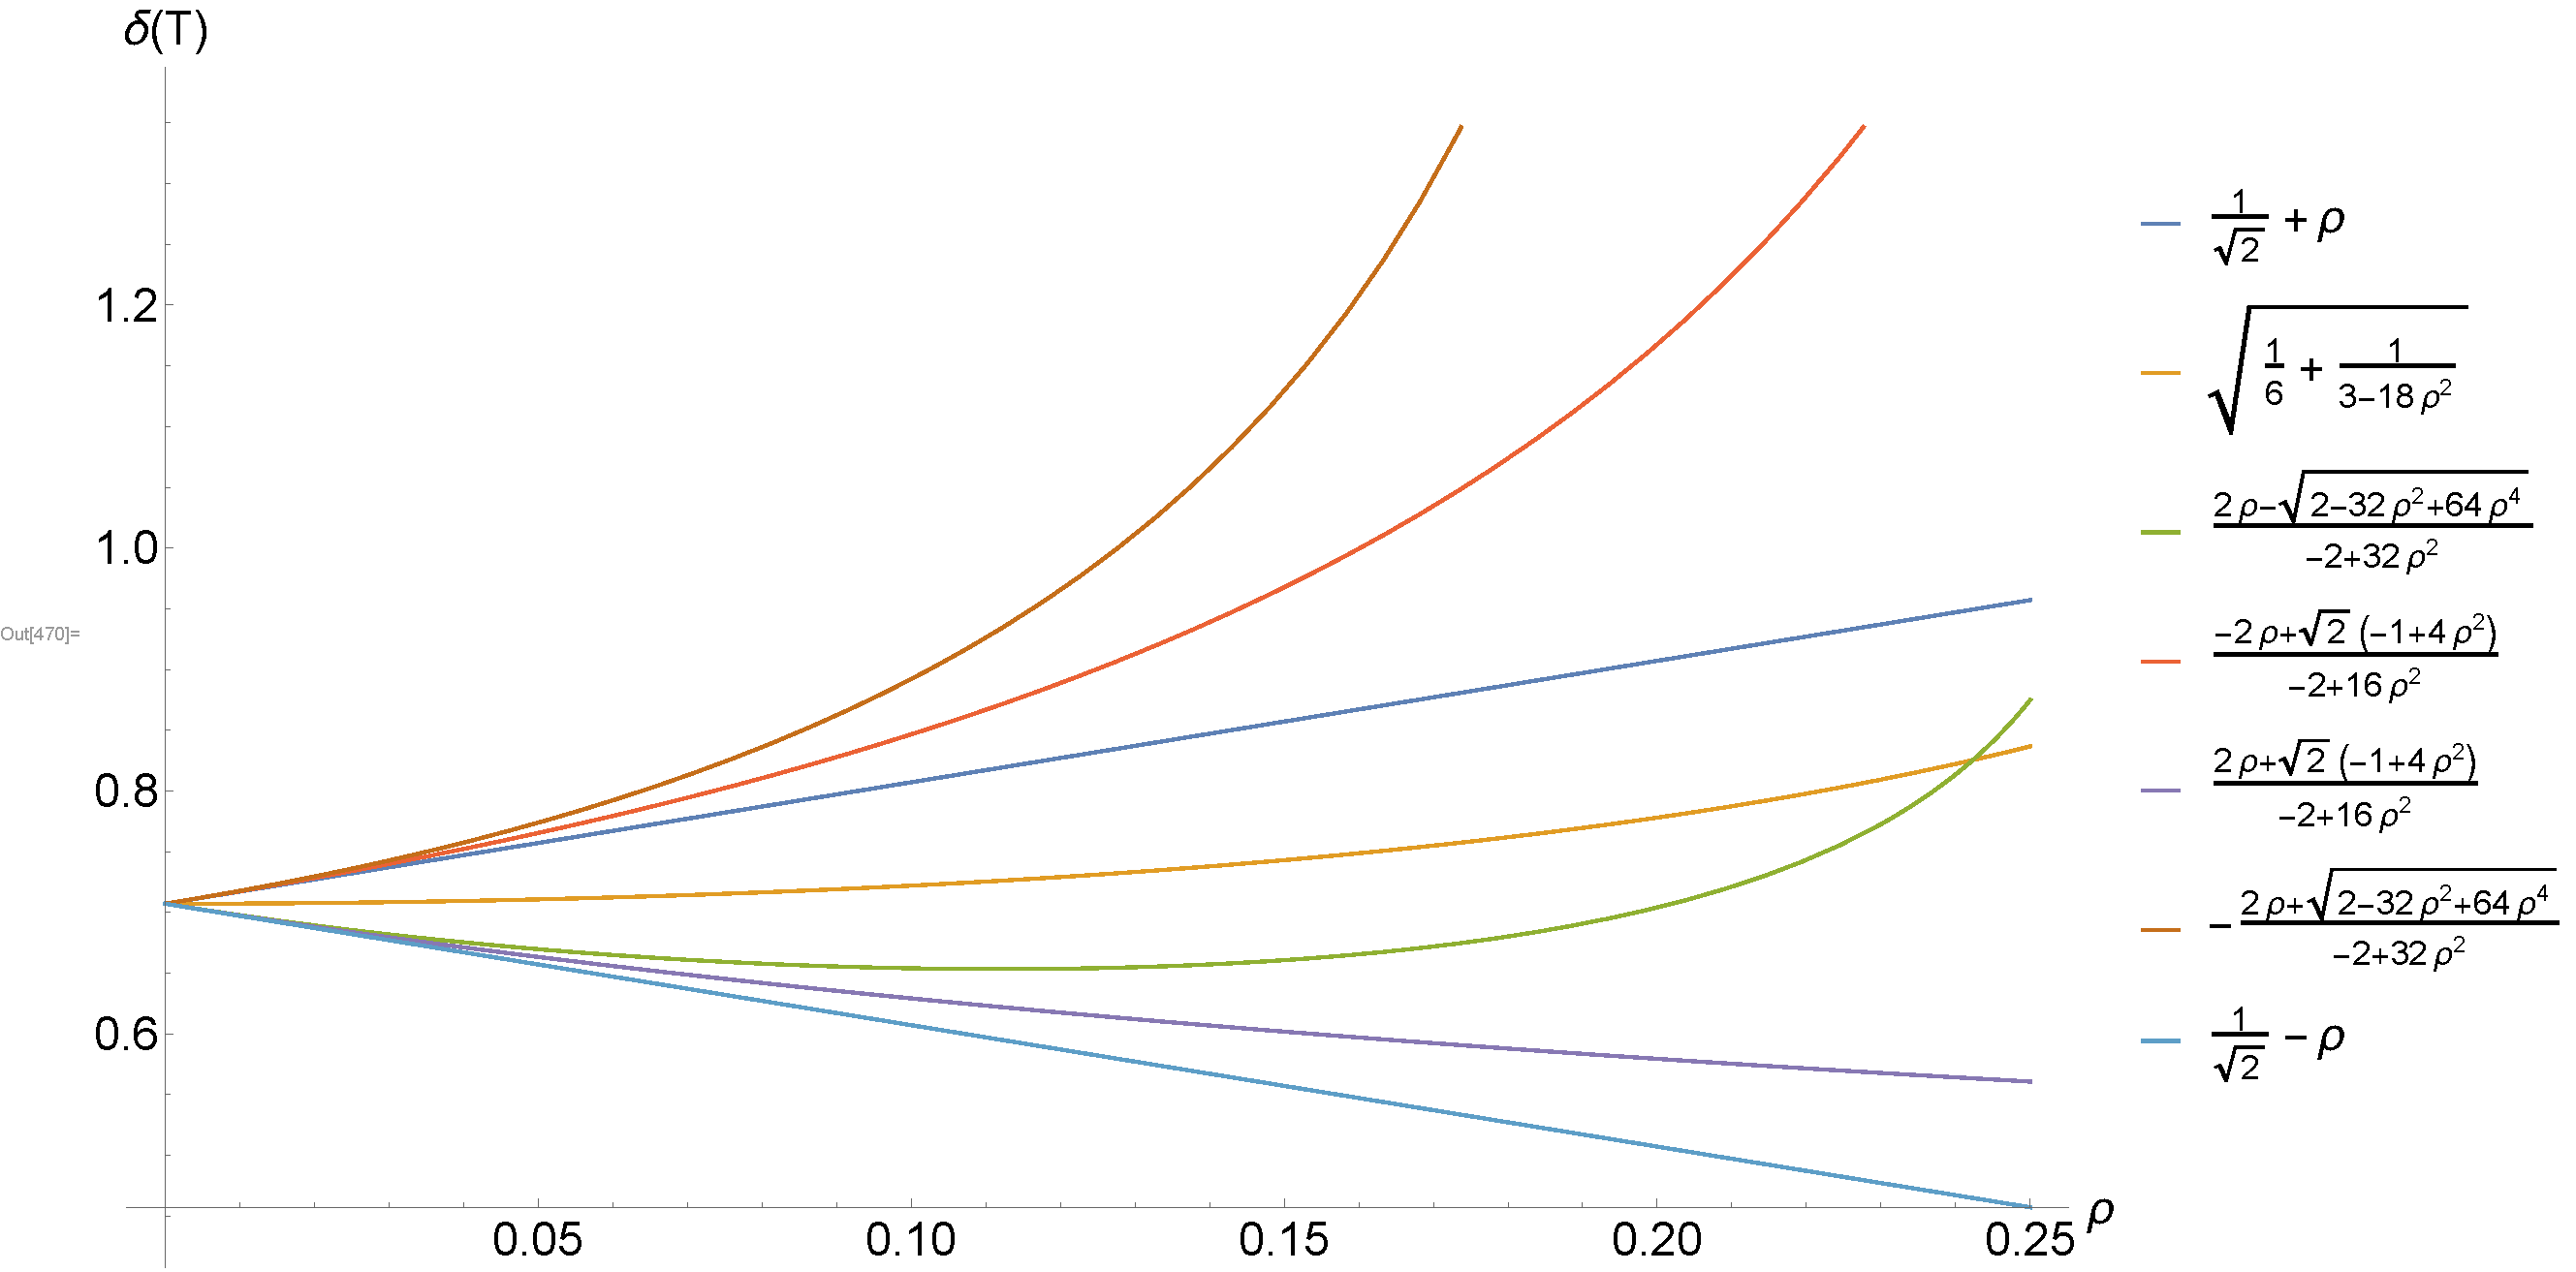
\includegraphics[width=1\textwidth]{../img/t2.pdf}
	\caption{All solutions to Apollonius problem with $T_2$, $a=1$}\label{fig:Apollonius2}
\end{figure}

\chapter{Appendix: Implementation details}\label{appendix:implementation}
\subsubsection{C++ and CGAL}
The MCMC procedure introduced in Chapter \ref{ch:simulation}, as well as the maximum pseudolikelihood estimation procedure introduced in Chapter \ref{ch:estimation}, was implemented in \texttt{C++} using the Computational Geometry Algorithms Library (\cite{cgal}). In particular, the package for 3D-triangulations (\cite{cgal:3d-triang}) was used. CGAL provides an implementation of both Delaunay and Laguerre\footnote{Laguerre tetrahedrization is called the \textit{3D regular triangulation} in CGAL.} tetrahedrizations which allows both adding and removing points. 

The current implementation allows control of the model parameters as well as number of iterations through command line arguments. For anything else, alterations of the code are required, although many changes (such as specifications of the form of the potential) can be done quickly, as functions for various characteristics such as volume, surface area, minimum edge length, etc., are already implemented. 

Three files are outputted for each simulation: cell data and estimation results, the tetrahedrization itself, and a log of the MCMC procedure.

In the near future, a simple documentation will be provided. 

The latest version of the code is available at \url{https://github.com/DahnJ/Gibbs-Laguerre-Delaunay}. 

\subsubsection{Python analysis}
The \texttt{C++} program outputs cell data in a standard \texttt{csv} format. These were subsequently analyzed in Python using the Jupyter notebook environment. The notebook can be found in the same repository as the \texttt{C++} code in the folder \texttt{python}. 


\subsubsection{Wolfram Mathematica}
In Remark \ref{r:zMathematica} and in Theorem \ref{thm:Apollonius}, Wolfram Mathematica (\cite{Mathematica}) was used. The Mathematica notebooks are contained in the repository of this thesis, available at \url{https://github.com/DahnJ/Thesis} in the folder \texttt{mathematica}.



%%% Abbreviations used in the thesis, if any, including their explanation
%%% In mathematical theses, it could be better to move the list of abbreviations to the beginning of the thesis.


%%% Attachments to the master thesis, if any. Each attachment must be
%%% referred to at least once from the text of the thesis. Attachments
%%% are numbered.
%%%
%%% The printed version should preferably contain attachments, which can be
%%% read (additional tables and charts, supplementary text, examples of
%%% program output, etc.). The electronic version is more suited for attachments
%%% which will likely be used in an electronic form rather than read (program
%%% source code, data files, interactive charts, etc.). Electronic attachments
%%% should be uploaded to SIS and optionally also included in the thesis on a~CD/DVD.
%%% Allowed file formats are specified in provision of the rector no. 72/2017.


% \listoftodos
\openright
\end{document}
